%%%%%%%%%%%%%%%%%%%%%%%%%%%%%%%%%%%%%%%%%%%%%%%%%%%%%%%%%%%%%%%%%%%%%
%DIF LATEXDIFF DIFFERENCE FILE
%DIF DEL ./scratch/few_shot_learning_for_low_data_drug_discovery/paper/main.tex   Wed Sep 28 16:44:45 2022
%DIF ADD ./git/few_shot_learning_for_low_data_drug_discovery/paper/main.tex       Wed Sep 28 16:45:32 2022
%% This is a (brief) model paper using the achemso class
%% The document class accepts keyval options, which should include
%% the target journal and optionally the manuscript type.
%%%%%%%%%%%%%%%%%%%%%%%%%%%%%%%%%%%%%%%%%%%%%%%%%%%%%%%%%%%%%%%%%%%%%
\documentclass[journal=jcisd8,manuscript=article]{achemso} % jcisd8 for jcim
% \documentclass[journal=acscii,manuscript=article,layout=twocolumn]{achemso}

%%%%%%%%%%%%%%%%%%%%%%%%%%%%%%%%%%%%%%%%%%%%%%%%%%%%%%%%%%%%%%%%%%%%%
%% Place any additional packages needed here.  Only include packages
%% which are essential, to avoid problems later.
%%%%%%%%%%%%%%%%%%%%%%%%%%%%%%%%%%%%%%%%%%%%%%%%%%%%%%%%%%%%%%%%%%%%%
\usepackage{amsfonts}

\usepackage{chemformula} % Formula subscripts using \ch{}
\usepackage[T1]{fontenc} % Use modern font encodings

\setcounter{secnumdepth}{4}

%%%%%%%%%%%%%%%%%%%%%%%%%%%%%%%%%%%%%%%%%%%%%%%%%%%%%%%%%%%%%%%%%%%%%
%% If issues arise when submitting your manuscript, you may want to
%% un-comment the next line.  This provides information on the
%% version of every file you have used.
%%%%%%%%%%%%%%%%%%%%%%%%%%%%%%%%%%%%%%%%%%%%%%%%%%%%%%%%%%%%%%%%%%%%%
%%\listfiles

%%%%%%%%%%%%%%%%%%%%%%%%%%%%%%%%%%%%%%%%%%%%%%%%%%%%%%%%%%%%%%%%%%%%%
%% Place any additional macros here.  Please use \newcommand* where
%% possible, and avoid layout-changing macros (which are not used
%% when typesetting).
%%%%%%%%%%%%%%%%%%%%%%%%%%%%%%%%%%%%%%%%%%%%%%%%%%%%%%%%%%%%%%%%%%%%%
\newcommand*\mycommand[1]{\texttt{\emph{#1}}}

\newenvironment{datasoftware}{%
\section*{Data and Software Availability}%
}{}

%%%%%%%%%%%%%%%%%%%%%%%%%%%%%%%%%%%%%%%%%%%%%%%%%%%%%%%%%%%%%%%%%%%%%
%% Meta-data block
%% ---------------
%% Each author should be given as a separate \author command.
%%
%% Corresponding authors should have an e-mail given after the author
%% name as an \email command. Phone and fax numbers can be given
%% using \phone and \fax, respectively; this information is optional.
%%
%% The affiliation of authors is given after the authors; each
%% \affiliation command applies to all preceding authors not already
%% assigned an affiliation.
%%
%% The affiliation takes an option argument for the short name.  This
%% will typically be something like "University of Somewhere".
%%
%% The \altaffiliation macro should be used for new address, etc.
%% On the other hand, \alsoaffiliation is used on a per author basis
%% when authors are associated with multiple institutions.
%%%%%%%%%%%%%%%%%%%%%%%%%%%%%%%%%%%%%%%%%%%%%%%%%%%%%%%%%%%%%%%%%%%%%
\author{Daniel Vella}
\affiliation{Department of Artificial Intelligence, University of Malta, Msida, MSD 2080, Malta.}

\author{Jean-Paul Ebejer}
\email{jean.p.ebejer@um.edu.mt} %% JP: the PI address is used, because you address will
\affiliation{Department of Artificial Intelligence, University of Malta, Msida, MSD 2080, Malta.}
\altaffiliation{Centre for Molecular Medicine and Biobanking, University of Malta, Msida, MSD 2080, Malta.}

%%%%%%%%%%%%%%%%%%%%%%%%%%%%%%%%%%%%%%%%%%%%%%%%%%%%%%%%%%%%%%%%%%%%%
%% The document title should be given as usual. Some journals require
%% a running title from the author: this should be supplied as an
%% optional argument to \title.
%%%%%%%%%%%%%%%%%%%%%%%%%%%%%%%%%%%%%%%%%%%%%%%%%%%%%%%%%%%%%%%%%%%%%
% \title[An \textsf{achemso} demo]
\title
  {Few-Shot Learning for Low-Data Drug Discovery}

%%%%%%%%%%%%%%%%%%%%%%%%%%%%%%%%%%%%%%%%%%%%%%%%%%%%%%%%%%%%%%%%%%%%%
%% Some journals require a list of abbreviations or keywords to be
%% supplied. These should be set up here, and will be printed after
%% the title and author information, if needed.
%%%%%%%%%%%%%%%%%%%%%%%%%%%%%%%%%%%%%%%%%%%%%%%%%%%%%%%%%%%%%%%%%%%%%
\abbreviations{LBVS, Tox21, MUV, DUD-E}
\keywords{machine learning, few-shot learning, low-data, prototypical networks, relation networks, matching networks}

%%%%%%%%%%%%%%%%%%%%%%%%%%%%%%%%%%%%%%%%%%%%%%%%%%%%%%%%%%%%%%%%%%%%%
%% The manuscript does not need to include \maketitle, which is
%% executed automatically.
%%%%%%%%%%%%%%%%%%%%%%%%%%%%%%%%%%%%%%%%%%%%%%%%%%%%%%%%%%%%%%%%%%%%%
%DIF PREAMBLE EXTENSION ADDED BY LATEXDIFF
%DIF UNDERLINE PREAMBLE %DIF PREAMBLE
\RequirePackage[normalem]{ulem} %DIF PREAMBLE
\RequirePackage{color}\definecolor{RED}{rgb}{1,0,0}\definecolor{BLUE}{rgb}{0,0,1} %DIF PREAMBLE
\providecommand{\DIFadd}[1]{{\protect\color{blue}\uwave{#1}}} %DIF PREAMBLE
\providecommand{\DIFdel}[1]{{\protect\color{red}\sout{#1}}}                      %DIF PREAMBLE
%DIF SAFE PREAMBLE %DIF PREAMBLE
\providecommand{\DIFaddbegin}{} %DIF PREAMBLE
\providecommand{\DIFaddend}{} %DIF PREAMBLE
\providecommand{\DIFdelbegin}{} %DIF PREAMBLE
\providecommand{\DIFdelend}{} %DIF PREAMBLE
\providecommand{\DIFmodbegin}{} %DIF PREAMBLE
\providecommand{\DIFmodend}{} %DIF PREAMBLE
%DIF FLOATSAFE PREAMBLE %DIF PREAMBLE
\providecommand{\DIFaddFL}[1]{\DIFadd{#1}} %DIF PREAMBLE
\providecommand{\DIFdelFL}[1]{\DIFdel{#1}} %DIF PREAMBLE
\providecommand{\DIFaddbeginFL}{} %DIF PREAMBLE
\providecommand{\DIFaddendFL}{} %DIF PREAMBLE
\providecommand{\DIFdelbeginFL}{} %DIF PREAMBLE
\providecommand{\DIFdelendFL}{} %DIF PREAMBLE
%DIF LISTINGS PREAMBLE %DIF PREAMBLE
\RequirePackage{listings} %DIF PREAMBLE
\RequirePackage{color} %DIF PREAMBLE
\lstdefinelanguage{DIFcode}{ %DIF PREAMBLE
%DIF DIFCODE_UNDERLINE %DIF PREAMBLE
  moredelim=[il][\color{red}\sout]{\%DIF\ <\ }, %DIF PREAMBLE
  moredelim=[il][\color{blue}\uwave]{\%DIF\ >\ } %DIF PREAMBLE
} %DIF PREAMBLE
\lstdefinestyle{DIFverbatimstyle}{ %DIF PREAMBLE
	language=DIFcode, %DIF PREAMBLE
	basicstyle=\ttfamily, %DIF PREAMBLE
	columns=fullflexible, %DIF PREAMBLE
	keepspaces=true %DIF PREAMBLE
} %DIF PREAMBLE
\lstnewenvironment{DIFverbatim}{\lstset{style=DIFverbatimstyle}}{} %DIF PREAMBLE
\lstnewenvironment{DIFverbatim*}{\lstset{style=DIFverbatimstyle,showspaces=true}}{} %DIF PREAMBLE
%DIF END PREAMBLE EXTENSION ADDED BY LATEXDIFF

\begin{document}

%%%%%%%%%%%%%%%%%%%%%%%%%%%%%%%%%%%%%%%%%%%%%%%%%%%%%%%%%%%%%%%%%%%%%
%% The "tocentry" environment can be used to create an entry for the
%% graphical table of contents. It is given here as some journals
%% require that it is printed as part of the abstract page. It will
%% be automatically moved as appropriate.
%%%%%%%%%%%%%%%%%%%%%%%%%%%%%%%%%%%%%%%%%%%%%%%%%%%%%%%%%%%%%%%%%%%%%
% \begin{tocentry}

% Some journals require a graphical entry for the Table of Contents.
% This should be laid out ``print ready'' so that the sizing of the
% text is correct.

% Inside the \texttt{tocentry} environment, the font used is Helvetica
% 8\,pt, as required by \emph{Journal of the American Chemical
% Society}.

% The surrounding frame is 9\,cm by 3.5\,cm, which is the maximum
% permitted for  \emph{Journal of the American Chemical Society}
% graphical table of content entries. The box will not resize if the
% content is too big: instead it will overflow the edge of the box.

% This box and the associated title will always be printed on a
% separate page at the end of the document.

% \end{tocentry}

%%%%%%%%%%%%%%%%%%%%%%%%%%%%%%%%%%%%%%%%%%%%%%%%%%%%%%%%%%%%%%%%%%%%%
%% The abstract environment will automatically gobble the contents
%% if an abstract is not used by the target journal.
%%%%%%%%%%%%%%%%%%%%%%%%%%%%%%%%%%%%%%%%%%%%%%%%%%%%%%%%%%%%%%%%%%%%%
\begin{abstract}
	The discovery of new \DIFdelbegin \DIFdel{leads }\DIFdelend \DIFaddbegin \DIFadd{hits }\DIFaddend through ligand-based virtual screening in drug discovery is essentially a low-data problem, as data acquisition is both difficult and expensive. The \DIFaddbegin \DIFadd{requirement for large amounts of training data hinders the }\DIFaddend application of conventional machine learning techniques to this problem domain\DIFdelbegin \DIFdel{is hindered by the requirement for large amounts of training data. In this work , we explore }\DIFdelend \DIFaddbegin \DIFadd{. This work explores }\DIFaddend few-shot machine learning for \DIFdelbegin \DIFdel{lead optimisation and hit identification, in which we }\DIFdelend \DIFaddbegin \DIFadd{hit discovery and lead optimisation. We }\DIFaddend build on the state-of-the-art \DIFdelbegin \DIFdel{, }\DIFdelend and introduce two new metric-based meta-learning techniques, Prototypical and Relation Networks, to this problem domain. We also explore \DIFdelbegin \DIFdel{the use of different embeddings}\DIFdelend \DIFaddbegin \DIFadd{using different embeddings, namely extended-connectivity fingerprints (ECFP) and embeddings generated through graph convolutional networks (GCN), }\DIFaddend as inputs to neural networks for classification. \DIFdelbegin \DIFdel{We find that learned graph embeddings }\DIFdelend \DIFaddbegin \DIFadd{This study shows that learned embeddings through GCNs }\DIFaddend consistently perform better than extended-connectivity fingerprints for toxicity and LBVS experiments. We conclude that the effectiveness of few-shot learning is highly dependent on the nature of the data. Few-shot learning models struggle to perform consistently on MUV and DUD-E data, in which the active compounds are structurally distinct. However, on Tox21 data, the few-shot models perform well, and we find that Prototypical Networks outperform the \DIFdelbegin \DIFdel{state of the art, which is }\DIFdelend \DIFaddbegin \DIFadd{state-of-the-art }\DIFaddend based on the Matching Networks architecture. Additionally, training these networks is substantially faster (up to 190\%) and therefore \DIFdelbegin \DIFdel{take }\DIFdelend \DIFaddbegin \DIFadd{takes }\DIFaddend a fraction of the time to train for comparable, or better, results.
\end{abstract}


%%%%%%%%%%%%%%%%%%%%%%%%%%%%%%%%%%%%%%%%%%%%%%%%%%%%%%%%%%%%%%%%%%%%%
%% Start the main part of the manuscript here.
%%%%%%%%%%%%%%%%%%%%%%%%%%%%%%%%%%%%%%%%%%%%%%%%%%%%%%%%%%%%%%%%%%%%%
\section{Introduction}

We humans exhibit a remarkable ability to learn new concepts fast and efficiently. This ability is in stark contrast with conventional supervised machine learning, which is \DIFdelbegin \DIFdel{data hungry }\DIFdelend \DIFaddbegin \DIFadd{data-hungry }\DIFaddend and requires a plethora of data points to develop an effective model. Meta-learning reframes the traditional machine learning problem, allowing machine learning models to learn \DIFaddbegin \DIFadd{new problems by }\DIFaddend utilising only a few examples. Humans have an innate capability to \textit{learn how to learn}, and bridging this gap between human and machine learning is \DIFdelbegin \DIFdel{beneficial, particularly }\DIFdelend \DIFaddbegin \DIFadd{particularly beneficial }\DIFaddend in domains where data availability or acquisition is difficult, such as the drug-discovery domain. The \DIFdelbegin \DIFdel{main goal in the }\DIFdelend drug-discovery process\DIFdelbegin \DIFdel{is the identification and development of active compounds , }\DIFdelend \DIFaddbegin \DIFadd{'s primary goal is identifying and developing active compounds }\DIFaddend that exhibit therapeutic effects against biological targets. The drug-discovery process comes with exorbitant costs and resource expenditure, which can exceed one billion dollars and take up to 15 years to complete \cite{hughes2011principles}.
\DIFaddbegin 

\DIFaddend Moreover, data is also expensive and difficult to acquire, as this requires testing of numerous compounds both \textit{in-vitro} and\DIFdelbegin \DIFdel{(later) }\DIFdelend \DIFaddbegin \DIFadd{, much later, }\DIFaddend \textit{in-vivo}. Even upon identification of leads, attrition rates are high as the compound usually fails for other reasons such as poor absorption, distribution, metabolism, excretion, or toxicology (ADMET) characteristics \cite{waring2015analysis}. It is difficult to predict such characteristics \DIFdelbegin \DIFdel{about }\DIFdelend \DIFaddbegin \DIFadd{of }\DIFaddend the candidate molecule when only a small amount of related biological data is available. Therefore, the \DIFdelbegin \DIFdel{lead identification and optimisation step }\DIFdelend \DIFaddbegin \DIFadd{hist discovery, lead identification, and optimisation steps }\DIFaddend in drug discovery \DIFdelbegin \DIFdel{is }\DIFdelend \DIFaddbegin \DIFadd{are }\DIFaddend essentially a low-data problem \cite{altae2017low}\DIFdelbegin \DIFdel{, in contrast to conventional machine learning which is data-hungry}\DIFdelend . In recent years, the computer vision domain saw successful applications and advancements for low-data machine learning \cite{koch2015siamese, vinyals2016matching, snell2017prototypical, sung2018learning}. Few-shot learning relieves the burden of collecting large-scale labelled data and makes \DIFdelbegin \DIFdel{the learning of }\DIFdelend \DIFaddbegin \DIFadd{learning }\DIFaddend rare cases possible \cite{wang2020generalizing}. 

\begin{figure}
    \centering
    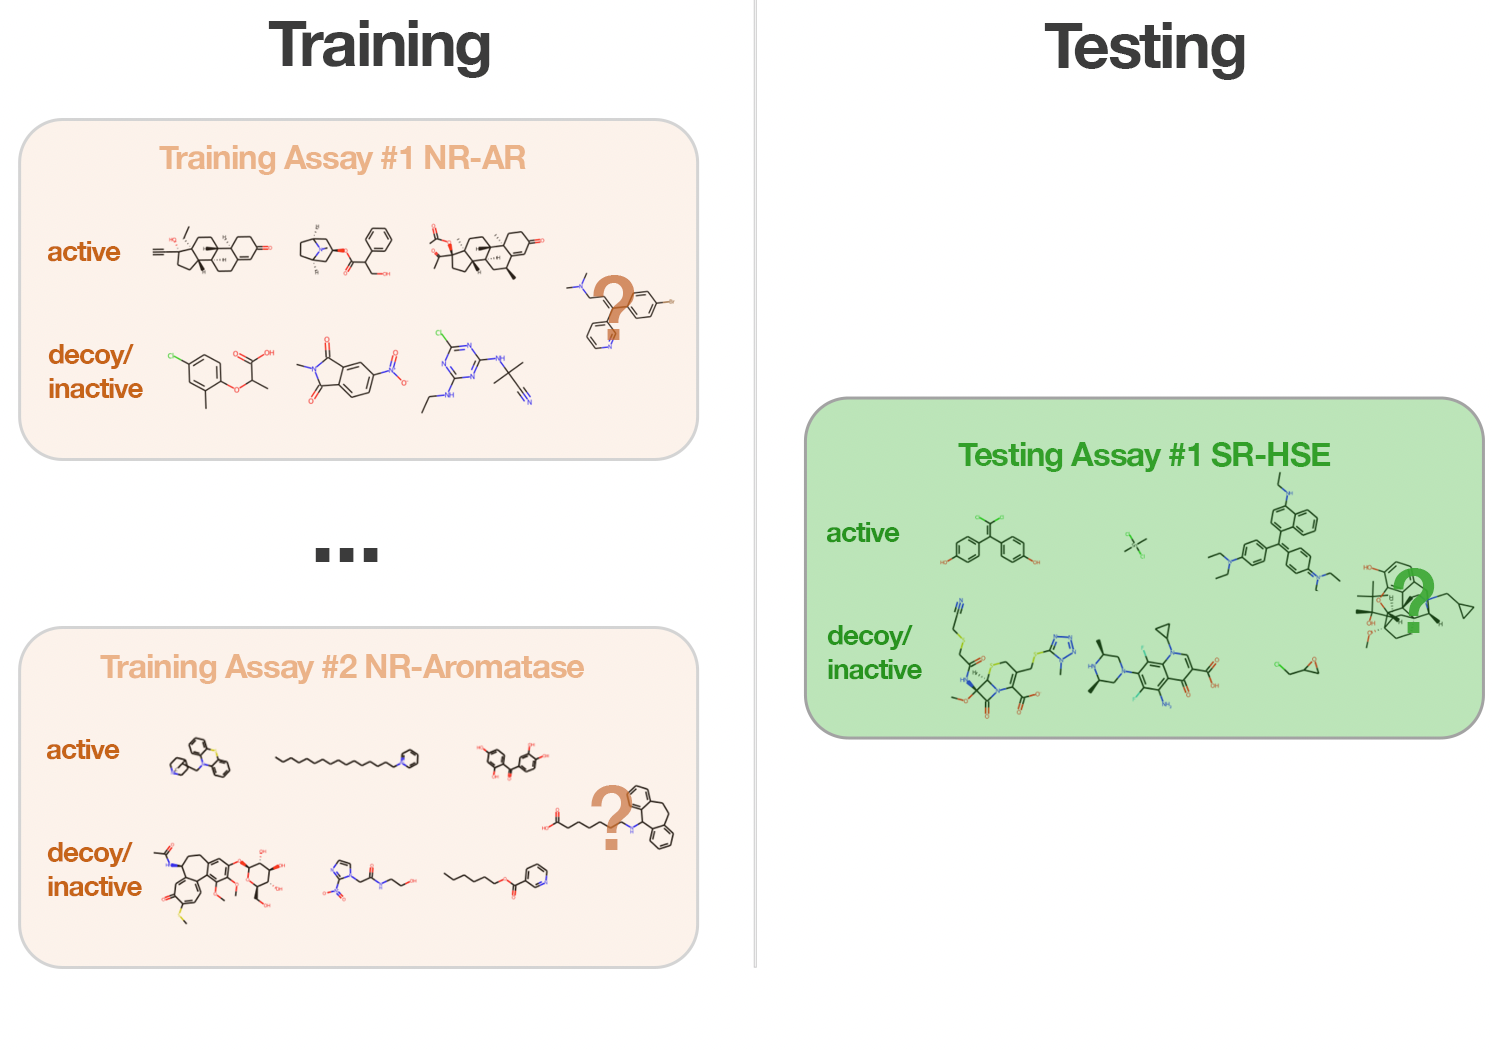
\includegraphics[width=0.8\linewidth]{img/tox21-metalearning.png}
    \caption{2-way 3-shot few-shot classification. Training a meta-learner on \DIFdelbeginFL \DIFdelFL{a set of }\DIFdelendFL experimental assays \DIFdelbeginFL \DIFdelFL{, }\DIFdelendFL and generalising for an unseen assay in the Tox-21 dataset.}
    \label{fig:tox21metalearning}
\end{figure}

Building on this notion, we \DIFdelbegin \DIFdel{aim to }\DIFdelend explore few-shot learning to address the low-data problem for hit \DIFdelbegin \DIFdel{identification and lead }\DIFdelend \DIFaddbegin \DIFadd{discovery, lead identification and }\DIFaddend optimisation. The ability \DIFdelbegin \DIFdel{for }\DIFdelend \DIFaddbegin \DIFadd{of }\DIFaddend a machine learning model to learn new concepts fast with just a few training examples is invaluable for this domain, where data on active compounds is scarce. Meta-learning aims to achieve generalising capabilities for \DIFdelbegin \DIFdel{environments that were previously unseen }\DIFdelend \DIFaddbegin \DIFadd{previously unseen environments }\DIFaddend during training time. \DIFdelbegin \DIFdel{Few-shot }\DIFdelend \DIFaddbegin \DIFadd{In few-shot }\DIFaddend classification, a meta-learning paradigm, we train models using a variety of training tasks and optimise \DIFdelbegin \DIFdel{for }\DIFdelend classification performance over a distribution of tasks, including unseen ones. Learning consists of a series of episodes, each consisting of an \textit{N}-way \textit{K}-shot classification task, effectively simulating the conditions at testing time. \DIFdelbegin \DIFdel{The }\textit{\DIFdel{way}} %DIFAUXCMD
\DIFdelend \DIFaddbegin \DIFadd{$N$ }\DIFaddend refers to the number of classes we \DIFdelbegin \DIFdel{have per taskand the }\textit{\DIFdel{shot}} %DIFAUXCMD
\DIFdel{component }\DIFdelend \DIFaddbegin \DIFadd{include per task, while $K$ }\DIFaddend refers to the number of \DIFdelbegin \DIFdel{samples. These samples }\DIFdelend \DIFaddbegin \DIFadd{molecules we sample for each class to }\DIFaddend make up the support set \cite{snell2017prototypical}. \DIFaddbegin \DIFadd{For this study, few-shot learning refers to training with as little as one example per class, referred to as one-shot learning \mbox{%DIFAUXCMD
\cite{koch2015siamese, vinyals2016matching}}\hspace{0pt}%DIFAUXCMD
, to a maximum of ten examples per class. }\DIFaddend During test time, a small support set is sampled from new, previously unseen targets, and \DIFaddbegin \DIFadd{the model uses }\DIFaddend these few data points \DIFdelbegin \DIFdel{are used by the model to generalise for the activity of query molecules}\DIFdelend \DIFaddbegin \DIFadd{to generalise query molecules' activity }\DIFaddend against this new target \cite{vinyals2016matching}. Figure~\ref{fig:tox21metalearning} shows an example of a typical meta-learning scenario on the Tox21 dataset \citep{huang2016tox21challenge}, where data from a set of assays reserved for training are used to train a model\DIFdelbegin \DIFdel{, which is later }\DIFdelend \DIFaddbegin \DIFadd{. This model is subsequently }\DIFaddend used to generalise for a \DIFdelbegin \DIFdel{new, }\DIFdelend \DIFaddbegin \DIFadd{previously }\DIFaddend unseen assay using only a \DIFaddbegin \DIFadd{small }\DIFaddend support set from this new assay. We highlight that few-shot learning in \DIFdelbegin \DIFdel{the hit identification and lead optimisation is different to other domains}\DIFdelend \DIFaddbegin \DIFadd{this problem domain differs from other domains, }\DIFaddend such as computer vision, where \DIFdelbegin \DIFdel{the trained model recognises }\DIFdelend \DIFaddbegin \DIFadd{a model is trained to recognise }\DIFaddend new classes. For example, given a few images of a lion\DIFdelbegin \DIFdel{as the support set}\DIFdelend , a class unseen during training, \DIFaddbegin \DIFadd{as the support set, }\DIFaddend the model must generalise for new images of a lion. In the domain under study, the challenge is to train a model that \DIFdelbegin \DIFdel{is able to }\DIFdelend \DIFaddbegin \DIFadd{can }\DIFaddend generalise for the behaviour of molecules in experimental assays which are related but not identical to the assays in the training collection, using only a small support set from \DIFdelbegin \DIFdel{this new experimental assay}\DIFdelend \DIFaddbegin \DIFadd{these new experimental assays}\DIFaddend . The molecules used during testing can thus be previously seen during training, but only in the context of their activity for different, but related experimental assays. Given a few molecules from new experimental assays, can the model predict the activity of molecules in this new assay using molecular data for different \DIFdelbegin \DIFdel{, but related , }\DIFdelend \DIFaddbegin \DIFadd{but related }\DIFaddend targets as training data?

Molecules are complex structures \DIFdelbegin \DIFdel{, }\DIFdelend consisting of atoms and bonds \DIFdelbegin \DIFdel{, and }\DIFdelend which must be somehow represented in computational space. The classical notation of compounds is the empirical formula such as $C_3H_7NO_2$\DIFdelbegin \DIFdel{, however, this holds no specific information on the molecule's topology. In fact, this particular formula }\DIFdelend \DIFaddbegin \DIFadd{. However, this }\DIFaddend can refer to alanine, sarcosine, \DIFdelbegin \DIFdel{and lactamide }\DIFdelend \DIFaddbegin \DIFadd{or lactamide as empirical formulae hold no information on a molecule's topology}\DIFaddend . Molecular representations such as Extended-Connectivity Fingerprints (ECFP) \cite{rogers2010extended}\DIFaddbegin \DIFadd{, }\DIFaddend and graph convolution learned embeddings \cite{duvenaud2015convolutional} embed more information than the empirical formula on the properties of the molecule\DIFdelbegin \DIFdel{, and can be used as inputs to machine learning networks. In this study , we mainly explore the use of }\DIFdelend \DIFaddbegin \DIFadd{. This study mainly explores using }\DIFaddend graphs as embeddings for the low-data machine learning networks.
\DIFdelbegin \DIFdel{A graph is formally defined as a set of nodes and a set of edges, where each edge connects a pair of nodes . This notion intuitively translates to molecular representations where atoms form }\DIFdelend \DIFaddbegin 

\DIFadd{A graph $G$ is a natural representation of a molecule, where nodes and edges represent atoms and bonds, respectively. When representing molecules, }\DIFaddend the set of \DIFdelbegin \DIFdel{nodes, and the bonds form }\DIFdelend \DIFaddbegin \DIFadd{vertices or nodes }\textit{\DIFadd{V}} \DIFadd{intuitively refers to atoms within a molecule, while }\DIFaddend the set of edges \DIFaddbegin \textit{\DIFadd{E}} \DIFadd{refers to the bonds that connect two atoms; such that $\mathcal{G}=(\mathcal{V}, \mathcal{E})$}\DIFaddend . Graphs are 2D objects, so spatial properties of a molecule\DIFaddbegin \DIFadd{, }\DIFaddend such as bond angles and chirality\DIFaddbegin \DIFadd{, }\DIFaddend are not inherent to the data object \DIFdelbegin \DIFdel{, }\DIFdelend but are instead encoded as node or edge attributes \cite{david2020molecular}. Embeddings of molecular graphs, augmented with atom feature information, can be learned using graph convolutional \DIFdelbegin \DIFdel{neural networks , which }\DIFdelend \DIFaddbegin \DIFadd{networks (GCNs). Selected properties such as atomic number, atom type, charge, and valences, among others, may be encoded in a node feature vector. \mbox{%DIFAUXCMD
\citet{wu2018moleculenet} }\hspace{0pt}%DIFAUXCMD
report that learned embeddings }\DIFaddend could be of benefit over topological molecular representations such as ECFP\DIFdelbegin \DIFdel{\mbox{%DIFAUXCMD
\cite{wu2018moleculenet}}\hspace{0pt}%DIFAUXCMD
}\DIFdelend .

In this study, we explore the application of several few-shot learning architectures including, in chronological order, Siamese Networks \citep{koch2015siamese}, Matching Networks \citep{vinyals2016matching}, Prototypical Networks \citep{snell2017prototypical}, and Relation Networks \citep{sung2018learning}. This group of architectures \DIFaddbegin \DIFadd{all }\DIFaddend fall under the umbrella of metric-based meta-learning. In our study, we embed molecule representations using \DIFdelbegin \DIFdel{graph convolution networks}\DIFdelend \DIFaddbegin \DIFadd{GCNs}\DIFaddend , and then use or learn a distance function over these embeddings. Effectively, metric-based learners seek to learn a relationship between the input embeddings in the task space. 
\DIFdelbegin \DIFdel{For the purposes of this study, few-shot learning refers to training with as little as one example per class, referred to as one-shot learning \mbox{%DIFAUXCMD
\cite{koch2015siamese, vinyals2016matching}}\hspace{0pt}%DIFAUXCMD
, to a maximum of ten examples per class. 
}\DIFdelend 

\section{Related Work}

Several successful research undertakings have exploited the low-data learning paradigm, especially in the computer-vision domain \cite{koch2015siamese, vinyals2016matching, snell2017prototypical, sung2018learning}. \DIFdelbegin \DIFdel{Being able to learn }\DIFdelend \DIFaddbegin \DIFadd{Learning }\DIFaddend from only a few examples is especially important in domains \DIFdelbegin \DIFdel{that suffer from }\DIFdelend \DIFaddbegin \DIFadd{with }\DIFaddend a paucity of data. This inaccessibility could be attributed to privacy, safety, or ethical issues \DIFdelbegin \DIFdel{, in addition to }\DIFdelend \DIFaddbegin \DIFadd{and }\DIFaddend other issues such as the time, resources and exorbitant costs associated with data acquisition. Learning with low-data can lead to less expensive data gathering\DIFaddbegin \DIFadd{, }\DIFaddend and reduced computational cost for learning \cite{wang2020generalizing}.

Building on past work in the metric-based meta-learning sphere \cite{vinyals2016matching}, \citet{altae2017low} introduce a deep-learning architecture for few-shot learning in drug discovery, in which they propose the iterative refinement long short-term memory (IterRefLSTM). IterRefLSTM builds on the Matching Networks \cite{vinyals2016matching} by introducing \DIFdelbegin \DIFdel{the Iterative Refinement }\DIFdelend \DIFaddbegin \DIFadd{iterative refinement }\DIFaddend of embeddings using Long-Short Term Memory (LSTM) networks. In our research, we build on the work by \DIFdelbegin \DIFdel{\mbox{%DIFAUXCMD
\citep{altae2017low} }\hspace{0pt}%DIFAUXCMD
}\DIFdelend \DIFaddbegin \DIFadd{\mbox{%DIFAUXCMD
\citet{altae2017low} }\hspace{0pt}%DIFAUXCMD
}\DIFaddend and extend it \DIFdelbegin \DIFdel{through the application of }\DIFdelend \DIFaddbegin \DIFadd{by applying }\DIFaddend other successful few-shot learning approaches \DIFdelbegin \DIFdel{, previously }\DIFdelend explored for other domains\DIFaddbegin \DIFadd{, }\DIFaddend such as the computer-vision domain. The authors employ Graph \DIFdelbegin \DIFdel{Neural Networks (GNN}\DIFdelend \DIFaddbegin \DIFadd{Convolutional Networks (GCN}\DIFaddend ) to learn molecular embeddings, which are then fed into the low-data architectures for classification.

\subsection{Graph \DIFdelbegin \DIFdel{Neural }\DIFdelend \DIFaddbegin \DIFadd{Convolutional }\DIFaddend Networks}

Molecules must be represented in computational space before processing them using few-shot machine learning techniques. \citet{wu2018moleculenet} report that graph-based models outperform conventional machine learning models on \DIFdelbegin \DIFdel{the majority of }\DIFdelend \DIFaddbegin \DIFadd{most }\DIFaddend datasets, suggesting that a learned embedding is advantageous over other molecular representations. \DIFdelbegin \DIFdel{Thus}\DIFdelend \DIFaddbegin \DIFadd{Building on this rationale}\DIFaddend , we opt for graph learned molecular representations to embed the input molecules \DIFdelbegin \DIFdel{. Graphs are natural representations of molecules, where nodes and edges represent atoms and bonds, respectively. When representing molecules, the set of vertices }\textit{\DIFdel{V}} %DIFAUXCMD
\DIFdel{intuitively refers to atoms within a molecule, while the set of edges }\textit{\DIFdel{E}} %DIFAUXCMD
\DIFdel{refers to the bonds that connects two atoms together (see Equation~\ref{eq_graph}). Selected properties such as atomic number, atom type, charge, and valences, amongst others, can be encoded in the node feature vector, in addition to bond information. However, the latter is omitted for the purpose of }\DIFdelend \DIFaddbegin \DIFadd{in }\DIFaddend this study. 

\DIFdelbegin \begin{displaymath}\DIFdel{\label{eq_graph}
	\mathcal{G}=(\mathcal{V}, \mathcal{E})
}\end{displaymath}%DIFAUXCMD
%DIFDELCMD < 

%DIFDELCMD < %%%
\DIFdel{Graph neural networks }\DIFdelend \DIFaddbegin \DIFadd{Graph Convolutional Networks (GCNs) }\DIFaddend may be used to learn molecular representations \cite{jiang2021could}. Embeddings learned through neural networks afford the construction of automated features \DIFdelbegin \DIFdel{, }\DIFdelend rather than fixed fingerprints. \DIFdelbegin \DIFdel{Graph neural networks }\DIFdelend \DIFaddbegin \DIFadd{GCNs }\DIFaddend transform small molecules into real-valued vector representations, which are an effective way of processing small molecules via deep neural networks \cite{gomez2018automatic}. \citet{duvenaud2015convolutional} report that using a differentiable method reduces collisions of substructures, and the learned embedding can be optimised to contain relevant features such as biological activity and substructure information.

If the graph object is our input signal, we can apply a set of operators to approximate the function we are attempting to learn. \citet{bronstein2021geometric} propose four key building blocks for deep learning on graphs, which include linear set equivariant layers, non-linear functions, local pooling layers\DIFaddbegin \DIFadd{, }\DIFaddend and set invariant layers. For graphs, the nodes $v$ are found on a domain $\Omega$ such that $v \in \Omega$. The nodes in $\Omega$ are stored in a feature space $C$, such that $C = \mathbb{R}^k$. Using a set of feature functions $X(\Omega, C)$, we can transform the feature space of the nodes in our domain. 

In the equivariant layer $B$, we can take the nodes in our domain and apply a function that transforms the features of the nodes such that $X(\Omega, C) \rightarrow X(\Omega', C')$. Equivariance allows for a function $g$ to be applied before or after this layer, such that $B(g.x) = g.B(x)$. The non-linear activation functions can be applied element-wise on the features of the nodes in a graph, such that $(\sigma(x))(v) = \sigma(x(v))$. Local pooling layers can be used to apply coarsening to the graph such that $X(\Omega, C) \rightarrow X(\Omega', C)$, in which we can reduce the number of nodes in our domain such that $\Omega' \subseteq \Omega$. Finally, we have the invariant layer $Z$, which can also be referred to as a global pooling layer, in which $X(\Omega, C) \rightarrow y$, which satisfies the invariant condition such that $Z(g.x) = Z(x)$ \citep{bronstein2021geometric}. Figure \ref{fig:neuralgraphfingerprint} illustrates an example of a \DIFdelbegin \DIFdel{GNN }\DIFdelend \DIFaddbegin \DIFadd{GCN }\DIFaddend to learn a molecular embedding.

\begin{figure}[h]
    \centering
    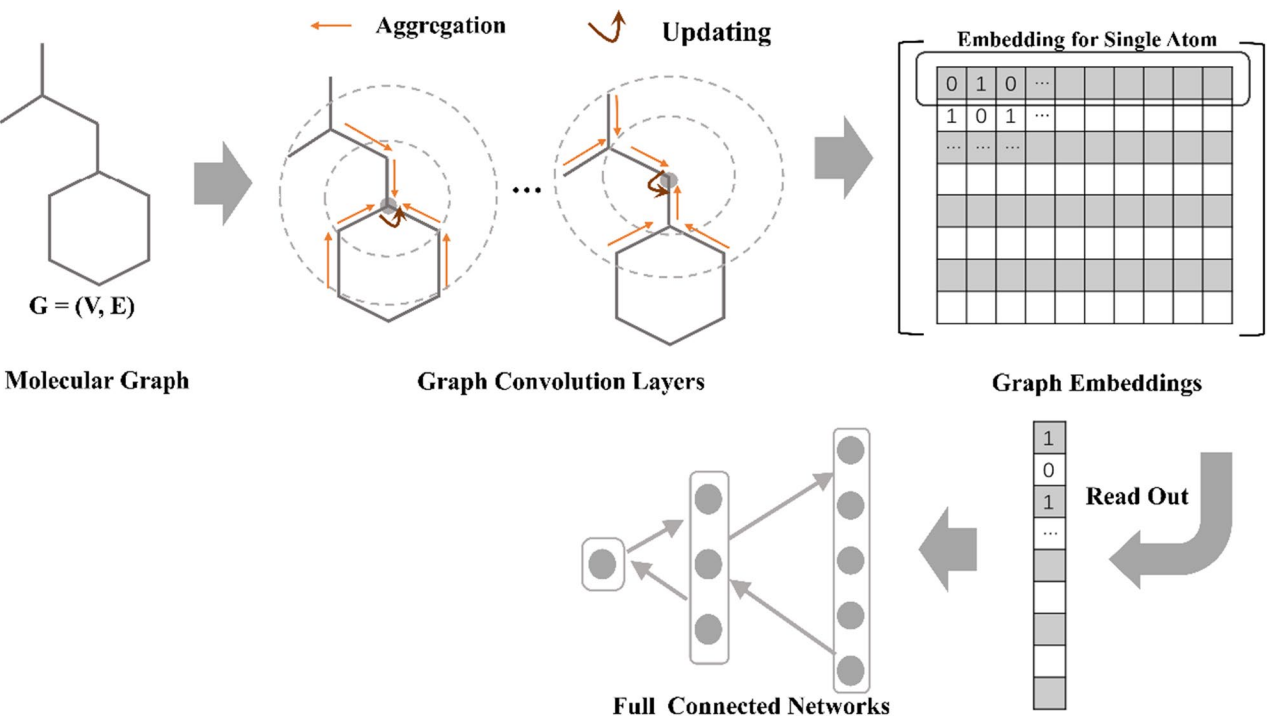
\includegraphics[width=0.9\linewidth]{img/graph_mol_embedding.png}
    \caption[Learned Embedding through a GCN]{A typical pipeline for representing molecules using a learned embedding function, which can be processed further using \DIFdelbeginFL \DIFdelFL{feed-forward }\DIFdelendFL \DIFaddbeginFL \DIFaddFL{feedforward }\DIFaddendFL neural networks as shown. Reproduced from \citet{jiang2021could}.}
    \label{fig:neuralgraphfingerprint}
  \end{figure}

\subsection{Metric-based Few-Shot Learning}

The success of a few-shot learning model for metric-based meta-learning is dependent on the effectiveness of a kernel $k_\theta$, which measures the similarity between data samples ${x..x_i}$ from a support set $S$ (see Equation \ref{kernel}) using a metric or distance function. The techniques employed in this study, excluding the benchmark model, use the support and query embeddings generated from the \DIFdelbegin \DIFdel{graph neural network }\DIFdelend \DIFaddbegin \DIFadd{GCNs }\DIFaddend to learn the kernel function. \DIFaddbegin \DIFadd{We explore four few-shot learning models in this study, which are presented in the Methodology section. These include Siamese Networks, Matching Networks (upon which the state-of-the-art is developed), Prototypical Networks and Relation Networks. The two latter networks are new approaches for this problem domain and are mostly inspired by the computer vision domain.
}\DIFaddend 

\begin{equation}
    \label{kernel}
    P_\theta(y \vert \mathbf{x}, S) = \sum_{(\mathbf{x}_i, y_i) \in S} k_\theta(\mathbf{x}, \mathbf{x}_i)y_i
\end{equation}

\subsubsection{Siamese Networks}

Siamese networks \DIFdelbegin \DIFdel{\mbox{%DIFAUXCMD
\cite{bromley1993signature, koch2015siamese} }\hspace{0pt}%DIFAUXCMD
}\DIFdelend \DIFaddbegin \DIFadd{\mbox{%DIFAUXCMD
\citep{koch2015siamese} }\hspace{0pt}%DIFAUXCMD
}\DIFaddend are composed of two identical networks \DIFdelbegin \DIFdel{, }\DIFdelend with shared weights and parameters, taking in a pair of data samples \DIFaddbegin \DIFadd{(molecules) }\DIFaddend as inputs. \DIFdelbegin \DIFdel{As the neural networks share weights, the feature extraction is maintained to the same feature space for both inputs. These identical subnetworks are finally connected in a final layerthat acts as a distance function for the two outputs.
    }\DIFdelend \DIFaddbegin \DIFadd{The distance between outputs from each component in the pair of networks is calculated to learn their relationship. The following is the process, repeated for all training tasks, employed for learning a classifier using Siamese Networks.
}\DIFaddend 

\begin{figure}[h]
    \centering
    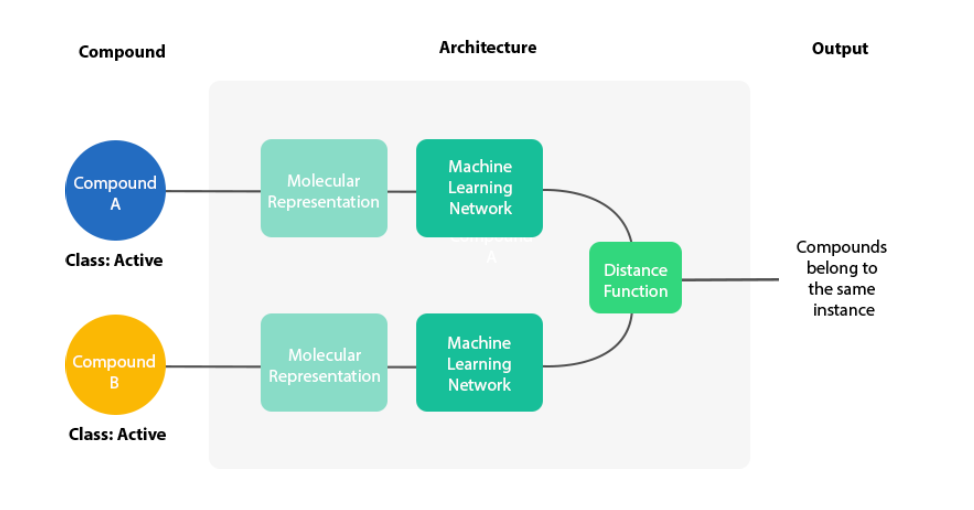
\includegraphics[width=0.9\linewidth]{img/high-level siamese.png}
    \DIFdelbeginFL %DIFDELCMD < \caption[High-level schematic of Siamese network]{%
{%DIFAUXCMD
\DIFdelFL{High level schematic of a Siamese network for molecular network. }%DIFDELCMD < \index{High Level Schematic of Siamese Network}%%%
}
	%DIFAUXCMD
\DIFdelendFL \DIFaddbeginFL \caption[High-level schematic of Siamese network]{\DIFaddFL{High-level schematic of a Siamese network for the molecular network.}}
    \DIFaddendFL \label{fig:siamesenetarchi}
\end{figure}

\DIFaddbegin \begin{enumerate}
    \item \DIFadd{Generate a list of all possible pairs between training data. If both data samples in the pair have the same target, the pair's label is set to one and zero if otherwise.
    }\item \DIFadd{Create a twin network using the GCN architecture to embed two molecular graph inputs into latent space.
    }\item \DIFadd{Calculate the L1 distance between the molecule embeddings. 
    }\item \DIFadd{The distance between the two embeddings is passed through a linear feedforward layer, followed by a sigmoid function to output the probability that the two molecules belong to the same class.
    }\item \DIFadd{The binary cross-entropy loss is calculated and backpropagated through the network.
}\end{enumerate}

\DIFaddend \subsubsection{Matching Networks}

\DIFdelbegin \DIFdel{Matching Networks \mbox{%DIFAUXCMD
\cite{vinyals2016matching} }\hspace{0pt}%DIFAUXCMD
build }\DIFdelend \DIFaddbegin \DIFadd{The Matching Networks architecture builds }\DIFaddend on Siamese Networks\DIFdelbegin \DIFdel{, but }\DIFdelend \DIFaddbegin \DIFadd{. However, }\DIFaddend instead of learning a metric function over \DIFdelbegin \DIFdel{pairs of data }\DIFdelend \DIFaddbegin \DIFadd{data pairs}\DIFaddend , the classifier learns how to define a probability distribution of output labels from query \DIFdelbegin \DIFdel{/test }\DIFdelend examples using a support set $S$. The classifier outputs a sum of \DIFdelbegin \DIFdel{attention weighted }\DIFdelend \DIFaddbegin \DIFadd{attention-weighted }\DIFaddend labels from the support set to predict the similarity between the \DIFdelbegin \DIFdel{test example and the samples from the support set }\DIFdelend \DIFaddbegin \DIFadd{query and the support set samples}\DIFaddend . We use the same embedding function for the support and query sets to compute the molecular embeddings. Subsequently, the cosine similarity \DIFdelbegin \DIFdel{between }\DIFdelend \DIFaddbegin \DIFadd{of }\DIFaddend pairs of data points between the support and query sets is computed, which is then normalised by a softmax function. The attention mechanism $a$ in $\hat{y} = \sum_{i=1}^{n} a(\hat{x}, x_i)y_i$ specifies how similar $\hat{x}$ is to each example $x$ in $S$.

\begin{figure}[!ht]
    \centering
    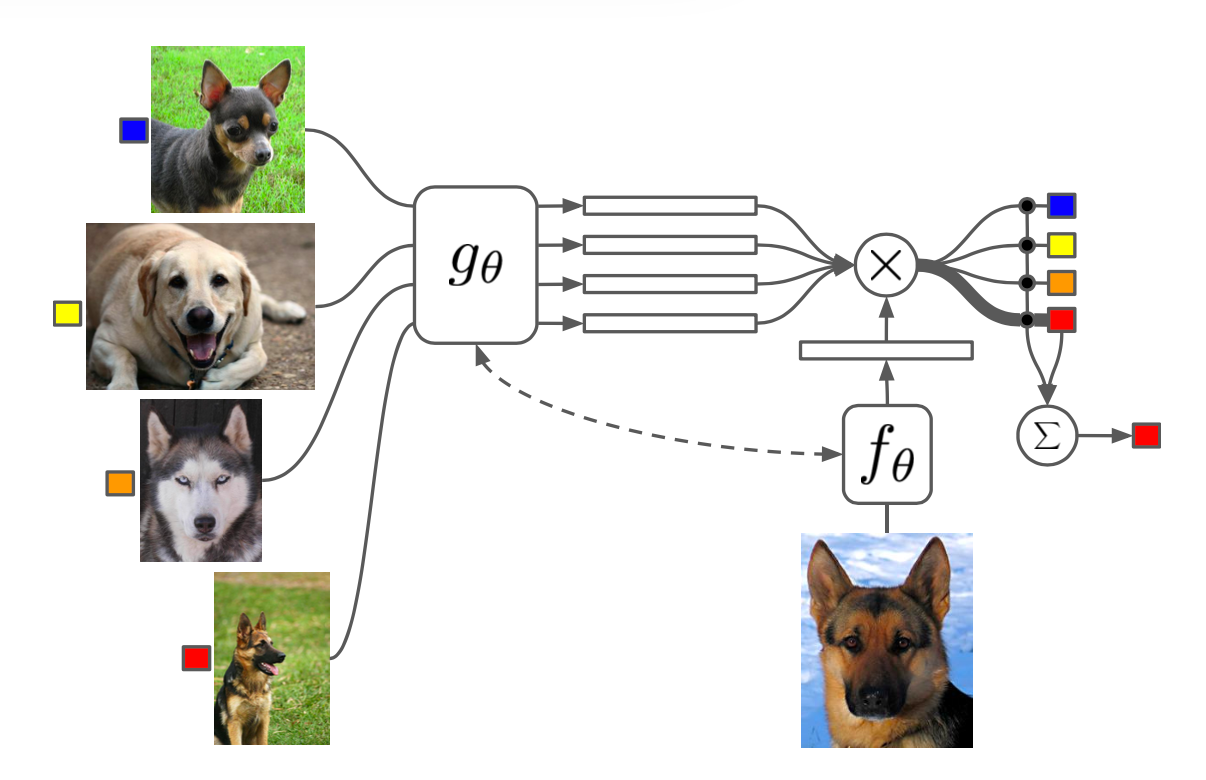
\includegraphics[width=0.7\linewidth]{img/matching_networks.png}
    \caption[Matching Networks Architecture]{Matching Networks Architecture. Reproduced from \citet{vinyals2016matching}.}
    \label{fig:matchingnets}
\end{figure}

Figure~\ref{fig:matchingnets} illustrates the Matching Nets architecture. Embedding functions $f$ and $g$ are Convolutional Neural Networks (CNNs) \citep{lecun1995convolutional}, potentially being identical to each other, which project the inputs to the feature space. \citet{vinyals2016matching} also propose full context embedding functions, which take as input the whole support set with the element $x_i$, thus resulting in \( g(x_i, S) \). Full context embeddings effectively modify how the element is embedded with respect to the whole support set $S$. A bidirectional LSTM is used to encode $x_i$ in the context of the support set. \DIFdelbegin \DIFdel{The }\DIFdelend \DIFaddbegin \DIFadd{Finally, the }\DIFaddend attention mechanism $a$, \DIFdelbegin \DIFdel{at the end of the pipeline, }\DIFdelend is the classifier which takes a softmax over the cosine distance of the embeddings. \DIFdelbegin %DIFDELCMD < 

%DIFDELCMD < %%%
\subsubsection{\DIFdel{Prototypical Networks}}
%DIFAUXCMD
\addtocounter{subsubsection}{-1}%DIFAUXCMD
%DIFDELCMD < 

%DIFDELCMD < %%%
\DIFdel{Prototypical Networks, proposed by \mbox{%DIFAUXCMD
\citet{snell2017prototypical}}\hspace{0pt}%DIFAUXCMD
, are similar to Matching Networks. Instead of comparing the query support to each support data point, a }\textit{\DIFdel{prototype}} %DIFAUXCMD
\DIFdel{is calculated}\DIFdelend \DIFaddbegin \DIFadd{As proposed in \mbox{%DIFAUXCMD
\citet{vinyals2016matching}}\hspace{0pt}%DIFAUXCMD
, fully contextual embeddings (FCE) are used in our implementation. Taking single data points to learn an embedding function limits the ability to embed the molecules effectively into latent space. Therefore, a bidirectional long-short term memory (LSTM) is used}\DIFaddend , which takes \DIFdelbegin \DIFdel{all the support data points per class and creates an embedding by averaging over }\DIFdelend the \DIFdelbegin \DIFdel{embeddings related to each class, thus creating the }\textit{\DIFdel{prototypes}}%DIFAUXCMD
\DIFdel{. The Euclidean distance between the query data point and the prototypes is calculated }\DIFdelend \DIFaddbegin \DIFadd{whole support set as input to adjust the embedding based on the other support samples. $g_\theta(x_i, S)$ encodes $x_i$, a data sample from the support set, in the context of the whole support set $S$. The LSTM transforms our support set embeddings by adding the forward and backward activations to the original support image embeddings. Subsequently, $f_\theta(x, S)$, encodes the query sample $x$ and trains the LSTM with read attention over the support set. The hidden state is updated over ten processing ``read'' steps until, eventually, the hidden state is equivalent to the aforementioned $f_\theta(x, S)$. The hidden state and the output from the attention function are updated in each iteration. The cross-entropy loss is computed for each query prediction whilst training the model using stochastic gradient descent.
}

\subsubsection{\DIFadd{Prototypical Networks}}

\DIFadd{Prototypical Networks \mbox{%DIFAUXCMD
\citep{snell2017prototypical} }\hspace{0pt}%DIFAUXCMD
have similarities to Matching Networks, but instead of considering the individual support set embeddings, the mean vector of the embeddings (referred to as the }\textit{\DIFadd{prototype}}\DIFadd{) for each class within the support set is taken. Another improvement \mbox{%DIFAUXCMD
\citet{snell2017prototypical} }\hspace{0pt}%DIFAUXCMD
make over Matching Networks is using Euclidean distance rather than the cosine distance to calculate the distances }\DIFaddend to classify the query (\DIFdelbegin \DIFdel{see }\DIFdelend \DIFaddbegin \DIFadd{refer to }\DIFaddend Figure~\ref{fig:protonets}). In \DIFdelbegin \DIFdel{a one-shot learning scenario, Prototypical Networks are equivalent to Matching Networks, however, the Euclidean distance is used instead of the Cosine distance used in Matching Networks.
}\DIFdelend \DIFaddbegin \DIFadd{order to classify query data samples, the softmax of the Euclidean distance's inverse between each query and each prototype is taken. The negative log-likelihood is used to train the network through stochastic gradient descent
}\DIFaddend 

\begin{figure}[!ht]
    \centering
    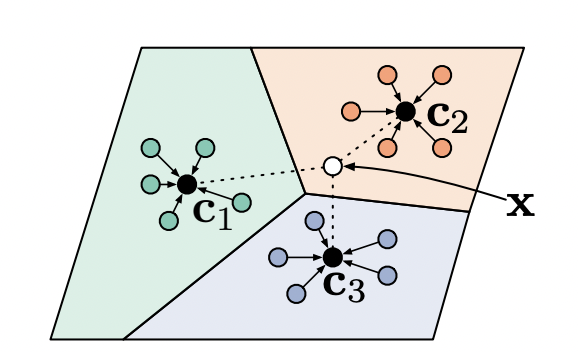
\includegraphics[width=0.7\linewidth]{img/protonets.png}
    \caption{Few-shot learning in Prototypical Networks, where prototypes \textbf{$c_k$} are taken as the mean of embedded support examples for each class. Reproduced from \citet{snell2017prototypical}.}
    \label{fig:protonets}
\end{figure}

\subsubsection{Relation Networks}

\citet{sung2018learning} present the Relation Network, a framework for few-shot learning, which could also be extended to zero-shot learning. The Relation Network learns a non-linear distance metric to compare support and query examples. \DIFdelbegin \DIFdel{As opposed to the aforementioned }\DIFdelend \DIFaddbegin \DIFadd{Unlike previously mentioned }\DIFaddend networks, this network uses a \DIFdelbegin \DIFdel{feed-forward }\DIFdelend \DIFaddbegin \DIFadd{feedforward }\DIFaddend neural network to learn a distance function in feature space. After embedding the support and query examples \DIFdelbegin \DIFdel{through }\DIFdelend \DIFaddbegin \DIFadd{using }\DIFaddend an embedding function, each query example is concatenated with each \DIFdelbegin \DIFdel{of the feature maps. The resulting }\DIFdelend \DIFaddbegin \DIFadd{feature map from the support set. The relationship between the queries and the different classes within the support set is captured by passing the }\DIFaddend feature map concatenations \DIFdelbegin \DIFdel{are processed using a convolutional neural network to output }\DIFdelend \DIFaddbegin \DIFadd{through a feed-forward neural network $g_\theta([x_i, x_j])$ to predict }\DIFaddend a relation score\DIFdelbegin \DIFdel{vector, from which the }\DIFdelend \DIFaddbegin \DIFadd{. The output }\DIFaddend class can be inferred \DIFdelbegin \DIFdel{(see Figure~\ref{fig:relationnets}) }\DIFdelend \DIFaddbegin \DIFadd{from this relation score vector. $[\cdot,\cdot]$ is the concatenation between each support set data sample $x_i$ and the query data samples $x_j$. The Mean Squared Error (MSE) is used as the loss function, as proposed in the original paper}\DIFaddend . 

\begin{figure}[h]
    \centering
    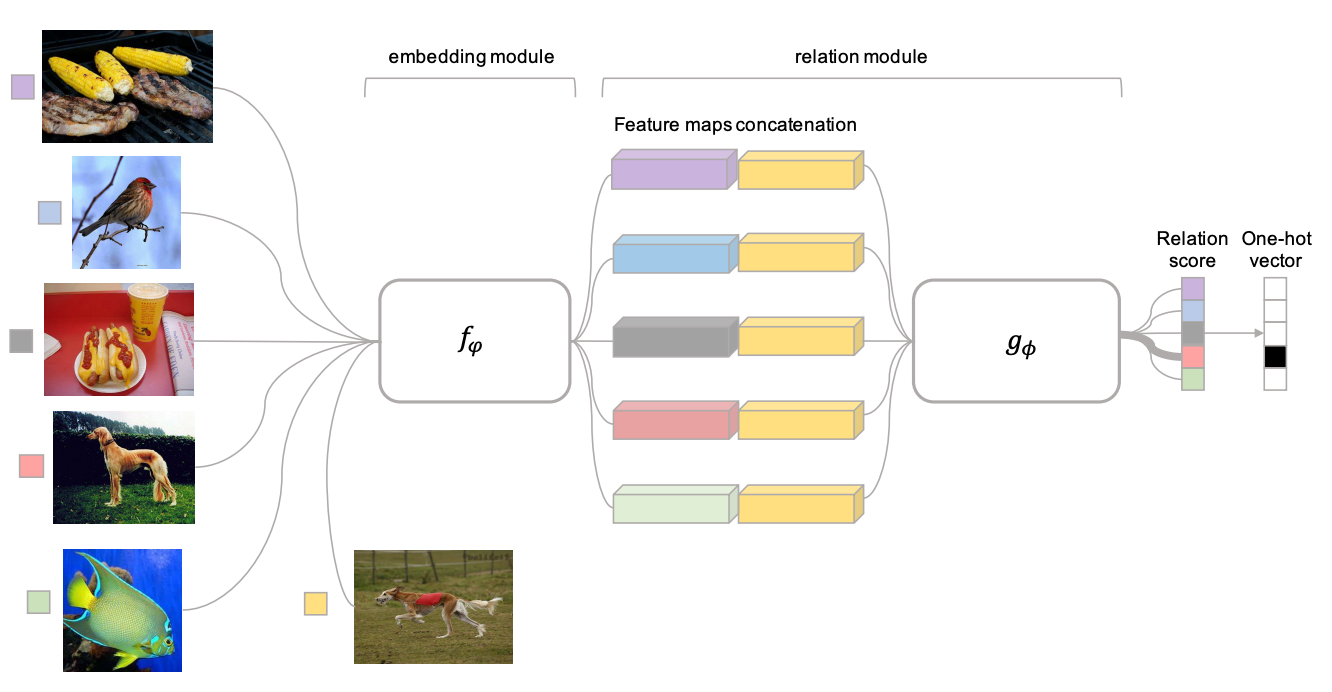
\includegraphics[width=0.9\linewidth]{img/relation-nets.png}
    \caption[Relation Networks]{Few-shot learning scenario in Relation Networks for a 5-way 1-shot learning task with one query as an example. Reproduced from \citet{sung2018learning}.}
    \label{fig:relationnets}
\end{figure}

\subsection{Iterative Refinement LSTM}

\citet{altae2017low} build on meta-learning concepts \DIFdelbegin \DIFdel{, where they train }\DIFdelend \DIFaddbegin \DIFadd{by training }\DIFaddend machine learning models on molecular data from a set of experimental assay targets (from the Tox21, SIDER, and MUV datasets) reserved for training. The model is then used to generalise for the activity of molecules in new, previously unseen experimental assays using only a small support set from \DIFdelbegin \DIFdel{the new assay}\DIFdelend \DIFaddbegin \DIFadd{these new assays}\DIFaddend . These test assays are related \DIFdelbegin \DIFdel{, }\DIFdelend but not identical \DIFdelbegin \DIFdel{, }\DIFdelend to the ones reserved for training. The number of molecules sampled for each class in the support set ranges from one to a maximum of ten molecules. \DIFdelbegin \DIFdel{In their work, the }\DIFdelend \DIFaddbegin \DIFadd{The }\DIFaddend support and query molecules are embedded \DIFaddbegin \DIFadd{in their work }\DIFaddend using a graph convolutional network. Bond information and distinction between bond types was not considered in their study. We note that the \textit{pool} layers do not coarsen the graphs \DIFdelbegin \DIFdel{, but simply }\DIFdelend \DIFaddbegin \DIFadd{but only }\DIFaddend apply a max function over neighbouring nodes.

\citet{altae2017low} propose the iterative refinement long-short term memory (IterRefLSTM) to further process the resulting embeddings in a few-shot machine learning pipeline. In IterRefLSTMs two embedding functions $f(\dot|S)$ and $g(\dot|S)$ are developed simultaneously. Therefore, the \DIFdelbegin \DIFdel{embedding of the query }\DIFdelend \DIFaddbegin \DIFadd{query embedding }\DIFaddend is built iteratively with that of the support set, using information from the two sets to enhance both the support and query embeddings. Once the embeddings have been iteratively refined, the authors apply a metric-based function to classify the queries using the support set embeddings. To emulate the Matching Networks, the authors \DIFdelbegin \DIFdel{make use of }\DIFdelend \DIFaddbegin \DIFadd{use }\DIFaddend the Cosine distance to compare embeddings. Figure \ref{fig:schematiconeshotdrug} illustrates a one-shot learning scenario encapsulating the \DIFdelbegin \DIFdel{aforementioned concepts }\DIFdelend \DIFaddbegin \DIFadd{concepts mentioned earlier}\DIFaddend .

\begin{figure}[h]
    \centering
    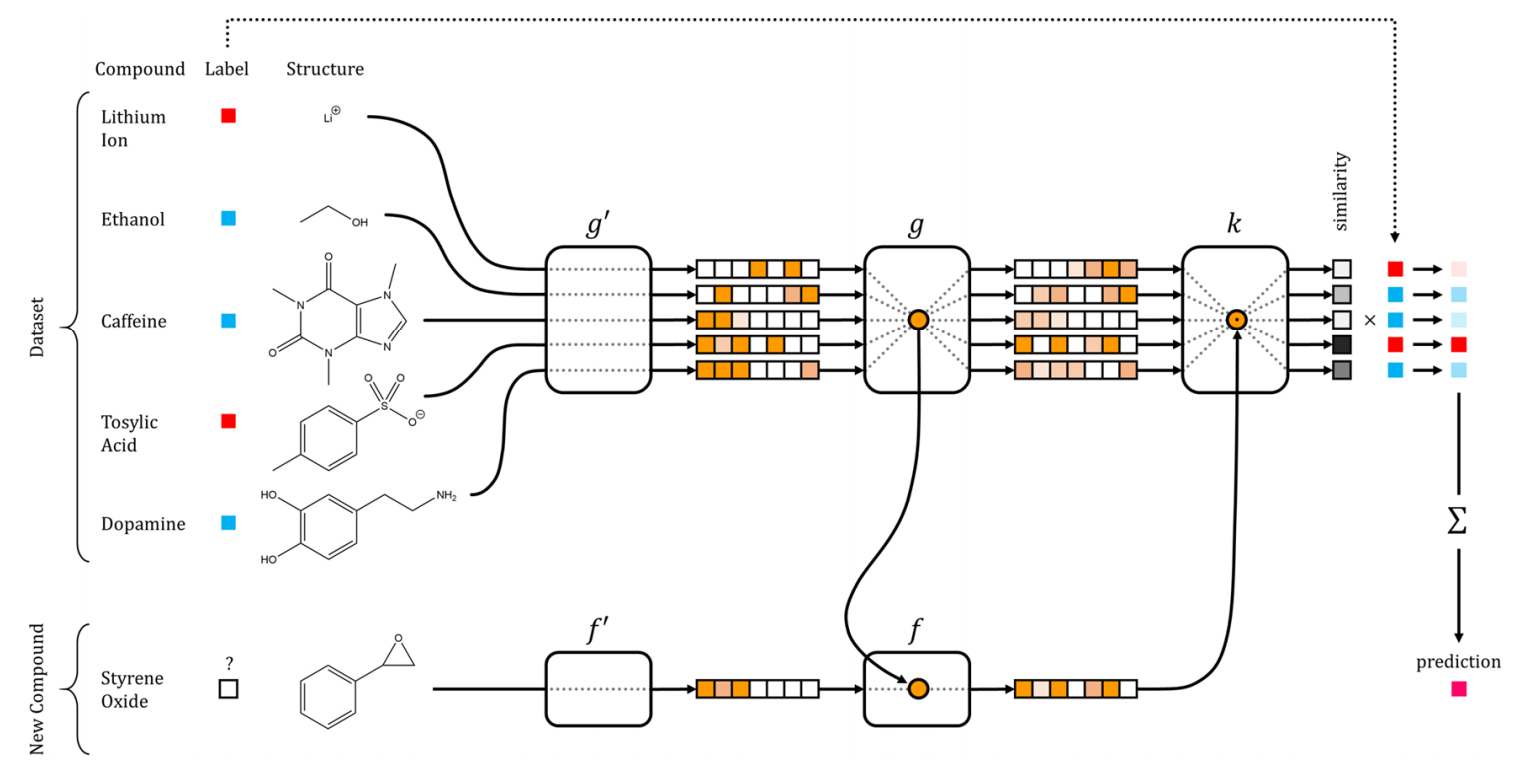
\includegraphics[width=0.9\linewidth]{img/pandeschematic.png}
    \caption[Schematic of one-shot learning in drug discovery]{Schematic of one-shot learning in drug discovery based on the Matching Network \citep{vinyals2016matching} architecture. Reproduced from \citet{altae2017low}.}
    \label{fig:schematiconeshotdrug}
\end{figure}

Their work is \DIFdelbegin \DIFdel{evaluation }\DIFdelend \DIFaddbegin \DIFadd{evaluated }\DIFaddend on the Tox21, the Side Effect Resource (SIDER) \citep{kuhn2016sider}, and MUV datasets\citep{rohrer2009maximum}. For every dataset, a subset of the targets is reserved for training and the rest for testing. Training is carried out as explained in the Matching Networks paper, in which training conditions match those at test time \citep{vinyals2016matching}. The authors \DIFdelbegin \DIFdel{make use of }\DIFdelend \DIFaddbegin \DIFadd{use }\DIFaddend a Random Forest (RF) with 100 decision trees as a machine learning baseline model. They also utilise a conventional Graph Convolutional Networks (GCN) \citep{kipf2016semi} as an additional baseline model, which is trained using only a small support set from the test targets. They then experiment with Siamese Networks \citep{koch2015siamese}, Matching Networks \citep{vinyals2016matching}, and an adaptation of the Matching Networks by applying the iterative refinement concepts explained earlier.

The authors utilise ROC-AUC scores to report the performance of the models. Considering the extreme imbalance of the data in the utilised datasets, \DIFaddbegin \DIFadd{favouring the negative (inactive/decoy) class, }\DIFaddend we note that the PR-AUC score would be a more appropriate evaluation measure. PR-AUC is based on the relationship between precision and recall, providing a clearer picture \DIFdelbegin \DIFdel{into }\DIFdelend \DIFaddbegin \DIFadd{of }\DIFaddend how the model performs when predicting the \textit{positive} (active) class in the data. \DIFdelbegin \DIFdel{Predicting }\DIFdelend \DIFaddbegin \DIFadd{Correctly predicting }\DIFaddend the ``active'' class \DIFdelbegin \DIFdel{correctly }\DIFdelend is of significant importance in virtual screening.

On the Tox21 and SIDER datasets, their proposed machine learning architecture achieves good ROC-AUC performance. The mean score for 10-shot learning on the median held-out task on Tox21 achieves a score of $0.823 \pm 0.002$, while for one-shot learning\DIFaddbegin \DIFadd{, }\DIFaddend the model achieves a mean score of $0.827 \pm 0.001$. The reasons why one-shot learning achieved better performance than 10-shot learning is uncertain, as we expect the model to perform better with larger support sets. However, this might be attributed to variance in the data between experiments. On MUV data, the baseline machine learning models \DIFdelbegin \DIFdel{out-performed }\DIFdelend \DIFaddbegin \DIFadd{performed }\DIFaddend few-shot learning. The authors report that this is due to MUV data being maximally informative\DIFdelbegin \DIFdel{, and therefore}\DIFdelend \DIFaddbegin \DIFadd{; therefore, }\DIFaddend structural similarity cannot be utilised to generalise \DIFdelbegin \DIFdel{for }\DIFdelend activity prediction. The authors open-sourced their models in the DeepChem library\citep{ramsundar2019deep}. However, the implementations are now outdated and \DIFdelbegin \DIFdel{not executable with the more recent versions of the DeepChem library, which makes reproduction of results difficult}\DIFdelend \DIFaddbegin \DIFadd{we were unable to train and test these models using the provided scripts}\DIFaddend . However, we study the open-sourced implementation \DIFdelbegin \DIFdel{along with the implementation }\DIFdelend \DIFaddbegin \DIFadd{and the respective }\DIFaddend details in the original literature to \DIFdelbegin \DIFdel{successfully reproduce this work }\DIFdelend \DIFaddbegin \DIFadd{reproduce their work successfully}\DIFaddend .

\section{Methodology}

\DIFdelbegin \DIFdel{In this work }\DIFdelend \DIFaddbegin \DIFadd{Building on the work of \mbox{%DIFAUXCMD
\citet{altae2017low}}\hspace{0pt}%DIFAUXCMD
}\DIFaddend , we implement a Random Forest and a \DIFdelbegin \DIFdel{Graph Convolutional Network (GCN ) to use }\DIFdelend \DIFaddbegin \DIFadd{GCN }\DIFaddend as benchmark models. Additionally, we implement four few-shot machine learning architectures\DIFdelbegin \DIFdel{, namely, }\DIFdelend \DIFaddbegin \DIFadd{: }\DIFaddend Siamese Networks, Matching Networks, Prototypical Networks, and Relation Networks. \DIFdelbegin \DIFdel{The state of the art, }\DIFdelend IterRefLSTMs \citep{altae2017low}, \DIFaddbegin \DIFadd{used in the state-of-the-art, }\DIFaddend are used to enrich the resulting embeddings in latent space. Molecules are represented as graph objects \DIFdelbegin \DIFdel{, which are then }\DIFdelend \DIFaddbegin \DIFadd{and subsequently }\DIFaddend processed using GCNs to produce a vectorised embedding in computational space. \DIFdelbegin \DIFdel{Throughout our work, we }\DIFdelend \DIFaddbegin \DIFadd{We }\DIFaddend try to follow the implementation of \citet{altae2017low} as closely as possible for \DIFdelbegin \DIFdel{the sake of }\DIFdelend reproducibility and homogenising \DIFdelbegin \DIFdel{the results for }\DIFdelend \DIFaddbegin \DIFadd{of results for effective }\DIFaddend comparison.

\subsection{Machine Learning Pipeline}

The machine learning pipeline for this study consists of nine main parts, which are illustrated in Figure~\ref{fig:architecture-schematic} and described hereunder:

\begin{enumerate}
    \item \textbf{Data Acquisition}. We utilise three main publicly available datasets for this study, namely, Tox21, MUV, and the GPCR subset of DUD-E. The \DIFdelbegin \DIFdel{data is provided }\DIFdelend \DIFaddbegin \DIFadd{latter is a new contribution to the study by \mbox{%DIFAUXCMD
\citet{altae2017low}}\hspace{0pt}%DIFAUXCMD
. All data is available }\DIFaddend as SMILES strings with a flag for the experimental assays in the dataset recording whether the molecule is active or an inactive/decoy.

    \item \textbf{Standardise molecule}. The SMILES strings are first standardised \DIFdelbegin \DIFdel{in order }\DIFdelend to transform all molecular representations according to a set of well-defined and consistent rules and conventions to ensure validity and uniformity.

    \item \textbf{Molecular features generation}. The molecular graph generated from the standardised SMILES representation is enriched with atom descriptors to add information to the molecular representation.

    \item \textbf{Molecular graphs generation}. The molecular representations \DIFdelbegin \DIFdel{we have so far }\DIFdelend are transformed into graph objects, consisting of nodes and edges representing atoms and bonds\DIFaddbegin \DIFadd{, }\DIFaddend respectively. The connectivity between atoms is represented via an adjacency matrix.

    \item \textbf{Episode generation}. Effective few-shot learning necessitates that conditions at training match those at testing \citep{vinyals2016matching}. Therefore, \DIFaddbegin \DIFadd{$N$-way $K$-shot }\DIFaddend support sets and queries are randomly sampled to form a series of episodes for training. \DIFdelbegin \DIFdel{The support sets are composed of a number of }\DIFdelend \DIFaddbegin \DIFadd{$K$ in each support set is constrained between one and ten }\DIFaddend examples per class. \DIFdelbegin \DIFdel{The number of examples per class ranges from just one example, up to ten examples}\DIFdelend \DIFaddbegin \DIFadd{For every episode, we have two classes, the active class and the inactive/decoy class. A subset of experimental assays in each dataset is reserved for training, while the rest are reserved for testing}\DIFaddend .

    \item \textbf{Learning a molecular embedding}. The sampled molecules \DIFdelbegin \DIFdel{in the episode }\DIFdelend \DIFaddbegin \DIFadd{from the current experimental assay }\DIFaddend are used to learn a molecular embedding using \DIFdelbegin \DIFdel{a graph convolutional network}\DIFdelend \DIFaddbegin \DIFadd{GCNs}\DIFaddend .

    \item \textbf{Few-Shot Learning}. The learned embeddings are processed using four different meta-learning architectures\DIFdelbegin \DIFdel{namely }\DIFdelend \DIFaddbegin \DIFadd{: }\DIFaddend Siamese, Matching, Prototypical and Relation Networks. \DIFdelbegin \DIFdel{Iterative Refinement LSTMs }\DIFdelend \DIFaddbegin \DIFadd{IterRefLSTMs }\DIFaddend \citep{altae2017low} are used to enrich the \DIFdelbegin \DIFdel{few-shot learning. A subset of experimental assays in each dataset is reserved for training, while the rest are reserved for testing}\DIFdelend \DIFaddbegin \DIFadd{model}\DIFaddend .  

    \item \textbf{Testing}. The trained models are subsequently used to test on new experimental assays, \DIFaddbegin \DIFadd{previously }\DIFaddend unseen during training, to gauge the generalising capability of a model trained for a low-data scenario. Support sets are randomly sampled and trained on the remaining molecules in the dataset for 20 rounds\DIFdelbegin \DIFdel{, for which the }\DIFdelend \DIFaddbegin \DIFadd{. The }\DIFaddend mean and standard deviation of the areas under the curve for Precision-Recall \DIFdelbegin \DIFdel{Curve }\DIFdelend \DIFaddbegin \DIFadd{(PR-AUC) }\DIFaddend and Receiver Operator Characteristic \DIFdelbegin \DIFdel{curve }\DIFdelend \DIFaddbegin \DIFadd{(ROC-AUC) }\DIFaddend are calculated to quantify performance.

    \item \textbf{Evaluation}. Finally, we evaluate the results based on the \DIFdelbegin \DIFdel{Receiver Operating Characteristic (ROC) and Precision Recall Area Under the Curves (}\DIFdelend \DIFaddbegin \DIFadd{ROC-AUC and }\DIFaddend PR-AUC \DIFdelbegin \DIFdel{) }\DIFdelend scores from the 20 test rounds. We apply statistical analysis for results obtained across different experiments to determine the \DIFdelbegin \DIFdel{best performing }\DIFdelend \DIFaddbegin \DIFadd{best-performing }\DIFaddend techniques for each support set composition. Confusion matrices, ROC-AUC and PR-AUC graphs for the experiment with the median ROC-AUC score from the 20 rounds are generated after test completion.
\end{enumerate}

\begin{figure}[!ht]
    \centering
    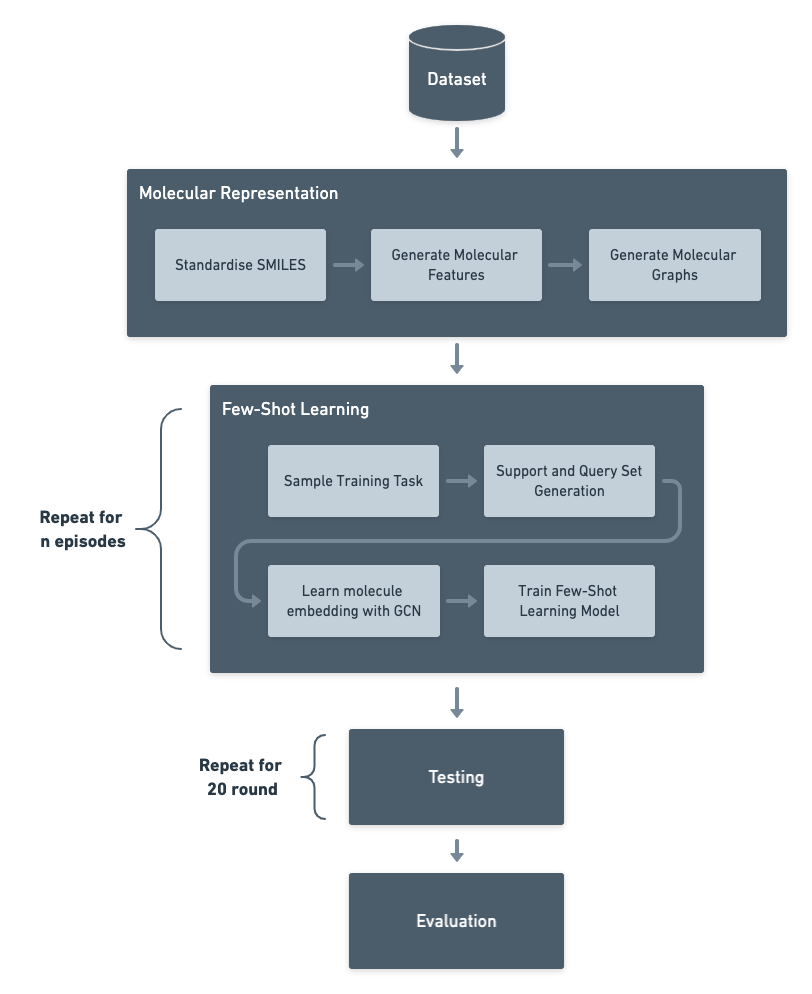
\includegraphics[width=0.9\linewidth]{img/architecture-schematic.png}
    \caption[Schematic of the major parts in our architecture]{Schematic of the machine learning pipeline designed for this study. The changes across few-shot learning architectures \DIFdelbeginFL \DIFdelFL{lies }\DIFdelendFL \DIFaddbeginFL \DIFaddFL{lie }\DIFaddendFL in the `Train Few-Shot Learning Model' component\DIFdelbeginFL \DIFdelFL{, otherwise}\DIFdelendFL \DIFaddbeginFL \DIFaddFL{. Otherwise}\DIFaddendFL , all other modules remain identical. \DIFaddbeginFL \DIFaddFL{Figure \ref{fig:schematiconeshotdrug} visualises the GCN learned embedding as }\textit{\DIFaddFL{g}}\DIFaddFL{' and }\textit{\DIFaddFL{f}}\DIFaddFL{', and the few-shot learning steps as }\textit{\DIFaddFL{g, f, k}}\DIFaddFL{.}\DIFaddendFL }
    \label{fig:architecture-schematic}
\end{figure}

\subsection{Datasets}

In this work, we make use of the following three datasets;

\begin{itemize}

    \item \textbf{Tox21} \citep{huang2016tox21challenge} -- Mainly used for lead optimisation, containing toxicity data for 12 targets \citep{tox21}. The dataset was obtained from the DeepChem AWS bucket\footnote{Accessed from: \url{https://deepchemdata.s3-us-west-1.amazonaws.com/datasets/tox21.csv.gz}. Last Accessed: 26/\DIFdelbegin \DIFdel{05}\DIFdelend \DIFaddbegin \DIFadd{09}\DIFaddend /2022} in CSV format. The NR-AR, NR-AR-LBD, NR-AhR, NR-Aromatase, NR-ER, NR-ER-LBD, NR-PPAR-gamma, SR-ARE, SR-ATAD5 targets are reserved for training, and the remaining SR-HSE, SR-MMP, SR-p53 targets are used for testing.

    \item \textbf{Maximum Unbiased Validation (MUV)} \citep{rohrer2009maximum} -- Based on PubChem BioAssays, used for validating virtual screening techniques against 17 different targets \citep{rohrer2009maximum}. The dataset was obtained from the DeepChem AWS bucket\footnote{Accessed from: \url{https://deepchemdata.s3-us-west-1.amazonaws.com/datasets/muv.csv.gz}. Last Accessed: 26/\DIFdelbegin \DIFdel{05}\DIFdelend \DIFaddbegin \DIFadd{09}\DIFaddend /2022} in CSV format. A total of 12 targets (MUV-466, MUV-548, MUV-600, MUV-644, MUV-652, MUV-689, MUV-692, MUV-712, MUV-713, MUV-733, MUV-737, and MUV-810) are reserved for training, while MUV-832, MUV-846, MUV-852, MUV-858, and MUV-859 are reserved for testing.

    \item \textbf{Directory of Useful Decoys (Enhanced) (DUD-E)} \cite{mysinger2012directory} -- Used for benchmarking virtual screening techniques by \DIFdelbegin \DIFdel{introducing a number of }\DIFdelend \DIFaddbegin \DIFadd{providing }\DIFaddend active compounds against specific \DIFdelbegin \DIFdel{targets. For each active, a number of }\DIFdelend \DIFaddbegin \DIFadd{protein targets. Many }\DIFaddend \textit{decoys} with similar physical properties \DIFdelbegin \DIFdel{, }\DIFdelend but different topologies \DIFdelbegin \DIFdel{, }\DIFdelend are made available \DIFdelbegin \DIFdel{. For this research study, we made use of }\DIFdelend \DIFaddbegin \DIFadd{for each active molecule. We used }\DIFaddend the GPCR subset of the DUD-E dataset \citep{mysinger2012directory} \DIFaddbegin \DIFadd{for this research study}\DIFaddend . The data was obtained directly from the DUD-E website.\footnote{Accessed from: \url{http://dude.docking.org/subsets/gpcr}. Last Accessed: 26/\DIFdelbegin \DIFdel{05}\DIFdelend \DIFaddbegin \DIFadd{09}\DIFaddend /2022} The AA2AR, DRD3, and ADRB1 targets are used for training. Two targets, ADRB2 and CXCR4, are reserved for testing. \DIFaddbegin \DIFadd{We note that this is an additional contribution to the study from \mbox{%DIFAUXCMD
\citet{altae2017low}}\hspace{0pt}%DIFAUXCMD
.
}\DIFaddend \end{itemize}

Table~\ref{table:datasetimbalance} shows the excessive imbalance of these datasets, highlighting the scarceness of data on active compounds in this domain. Due to this class imbalance\DIFdelbegin \DIFdel{we select appropriate performance metrics (see Evaluation Section)}\DIFdelend \DIFaddbegin \DIFadd{, we also report PR-AUC metrics in addition to the ROC-AUC metrics presented in the study by \mbox{%DIFAUXCMD
\citet{altae2017low}}\hspace{0pt}%DIFAUXCMD
}\DIFaddend .

\begin{table}[h]
    \centering
    \caption{Number of actives and inactives/decoys across all targets in the datasets used. Figures in parentheses show the percentage of the total compounds in the dataset.}
    \begin{tabular}{@{}crr@{}}
        \hline
        Dataset         & Actives           & Inactives/Decoys \\
        \hline
        Tox21           & 4,149 (7.04\%)    & 54,746 (92.96\%) \\
        MUV             & 347 (0.20\%)      & 175,990 (99.80\%) \\
        DUD-E (GPCR)    & 1,249 (1.45\%)    & 84,856 (98.55\%) \\
        \hline              
    \end{tabular}
    \label{table:datasetimbalance}
\end{table}

\subsection{Molecular Representations}

We first standardise the molecules according to \DIFdelbegin \DIFdel{a set of }\DIFdelend well-defined and consistent rules and conventions. \DIFdelbegin \DIFdel{It is of utmost importance to maintain }\DIFdelend \DIFaddbegin \DIFadd{Maintaining }\DIFaddend uniformity and integrity across the different \DIFdelbegin \DIFdel{datasets (and sources) being used}\DIFdelend \DIFaddbegin \DIFadd{data is of utmost importance}\DIFaddend . \citet{bento2020open} present an open source chemical structure curation pipeline based on RDKit\citep{rdkit} for validating and standardising chemical structures, which follow FDA/IUPAC guidelines \citep{brecher2006graphical, food2007substance}. Their work is available in the ChEMBL Structure Pipeline package \DIFdelbegin \DIFdel{\mbox{%DIFAUXCMD
\cite{bento2020open} }\hspace{0pt}%DIFAUXCMD
}\DIFdelend \DIFaddbegin \DIFadd{\mbox{%DIFAUXCMD
\citep{bento2020open} }\hspace{0pt}%DIFAUXCMD
}\DIFaddend and is used to standardise the molecules in our pipeline. 

We create a molecular graph from the SMILES string of the \DIFdelbegin \DIFdel{standardized }\DIFdelend \DIFaddbegin \DIFadd{standardised }\DIFaddend molecule using RDKit, an open-source toolkit for cheminformatics. We then one-hot encode eight \DIFdelbegin \DIFdel{features for the atoms }\DIFdelend \DIFaddbegin \DIFadd{atom features }\DIFaddend in each molecule\DIFdelbegin \DIFdel{, namely, }\DIFdelend \DIFaddbegin \DIFadd{: }\DIFaddend atom type, atomic number, atom degree, explicit valence, hybridisation, formal charge, number of radical electrons, and aromaticity. \DIFdelbegin \DIFdel{Self loops }\DIFdelend \DIFaddbegin \DIFadd{Self-loops }\DIFaddend are added to every node in the generated graph, so aggregation functions during message passing consider the features of the node itself. The order of the atoms follows the canonical order of the atoms assigned through RDKit. We make use of the Deep Graph Library (DGL) LifeSci \cite{dgllife} library to create the graph objects and subsequently process them using the DGL library \cite{wang2019dgl}.

\subsection{Episodic Learning}

\DIFdelbegin \DIFdel{Figure~\ref{fig:episodiclearning} illustrates a high-level overview of the episodic learning methodology. }\DIFdelend Training for few-shot learning is carried out in a series of episodes, \DIFdelbegin \DIFdel{framed as }\textit{\DIFdel{N-way K-shot}} %DIFAUXCMD
\DIFdel{classification tasks}\DIFdelend \DIFaddbegin \DIFadd{as shown in Figure \ref{fig:architecture-schematic}}\DIFaddend . We consider \DIFdelbegin \textit{\DIFdel{N-way K-shot}} %DIFAUXCMD
\DIFdel{classification tasks }\DIFdelend \DIFaddbegin \DIFadd{$N$-way $K$-shot classification tasks for each episode}\DIFaddend , where the support set contains \textit{N} classes and \textit{K} labelled molecules. \DIFdelbegin \DIFdel{These classification tasks match the conditions at training time with those during testing, as proposed by \mbox{%DIFAUXCMD
\citet{vinyals2016matching}}\hspace{0pt}%DIFAUXCMD
. }\DIFdelend The tasks in our research are binary classification tasks\DIFdelbegin \DIFdel{, therefore }\DIFdelend \DIFaddbegin \DIFadd{. Therefore }\DIFaddend \textit{N} is always set to two to represent the active and the inactive/decoy class\DIFaddbegin \DIFadd{, }\DIFaddend respectively. Experiments with varying values of \textit{K} are carried out to generate the support sets, with a minimum of one data point, to a maximum of ten data points (molecules) per class. The combinations for \textit{K} active and inactive/decoy classes are not exhaustive, but we follow the support set composition used in \citet{altae2017low} to \DIFdelbegin \DIFdel{directly compare results with this study }\DIFdelend \DIFaddbegin \DIFadd{compare our results with their study directly}\DIFaddend .

\DIFdelbegin %DIFDELCMD < \begin{figure}[ht!]
%DIFDELCMD < 	\centering
%DIFDELCMD < 	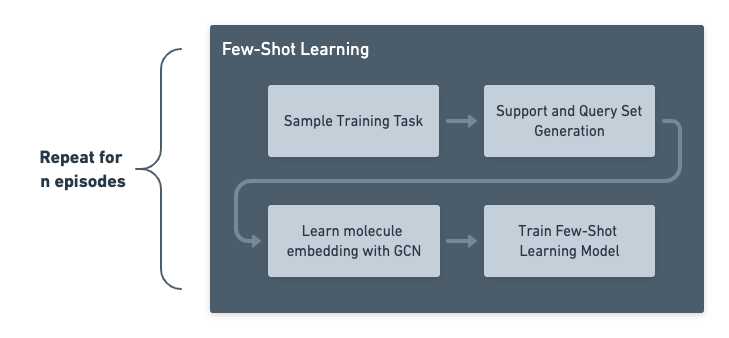
\includegraphics[width=0.9\linewidth]{img/episodic-learning.png}
%DIFDELCMD < 	%%%
%DIFDELCMD < \caption{%
{%DIFAUXCMD
\DIFdelFL{Episodic learning schematic}}
	%DIFAUXCMD
%DIFDELCMD < \label{fig:episodiclearning}
%DIFDELCMD < \end{figure}
%DIFDELCMD < 

%DIFDELCMD < %%%
\DIFdelend Table~\ref{table:support-set-sizes} contains the composition of the support sets used in our experiments. For each episode, we sample a total of 128 query molecules \DIFdelbegin \DIFdel{, which is }\DIFdelend composed of a balanced combination of molecules from each class. If the active class for a specific target contains less than 64 molecules, the active molecules are over-sampled such that each query set contains 64 actives. The choice of the support set composition was based on the methodology presented in \citet{altae2017low}.

\begin{table}
    \centering
    \begin{tabular}{@{}rrr@{}}
        \hline
        Actives & Inactives/Decoys & Support Set Size \\
        \hline
        10  & 10 & 20 \\
        5   & 10 & 15 \\
        1   & 10 & 11 \\
        1   & 5  & 6 \\
        1   & 1  & 2 \\
        \hline
    \end{tabular}
    \caption{Support set composition}
    \label{table:support-set-sizes}
\end{table}

\subsection{Machine Learning Models}

Before processing the molecular graph, the model first learns an embedding using \DIFdelbegin \DIFdel{graph neural networks}\DIFdelend \DIFaddbegin \DIFadd{GCNs}\DIFaddend . Four different architectures, including Siamese, Matching, Prototypical and Relation Networks, \DIFaddbegin \DIFadd{subsequently }\DIFaddend process the learned graph embeddings to train our meta-learner.
\DIFdelbegin \DIFdel{IterRefLSTMs are utilised to refine the latent space embeddings. 
}\DIFdelend 

\begin{figure}[ht!]
    \centering
    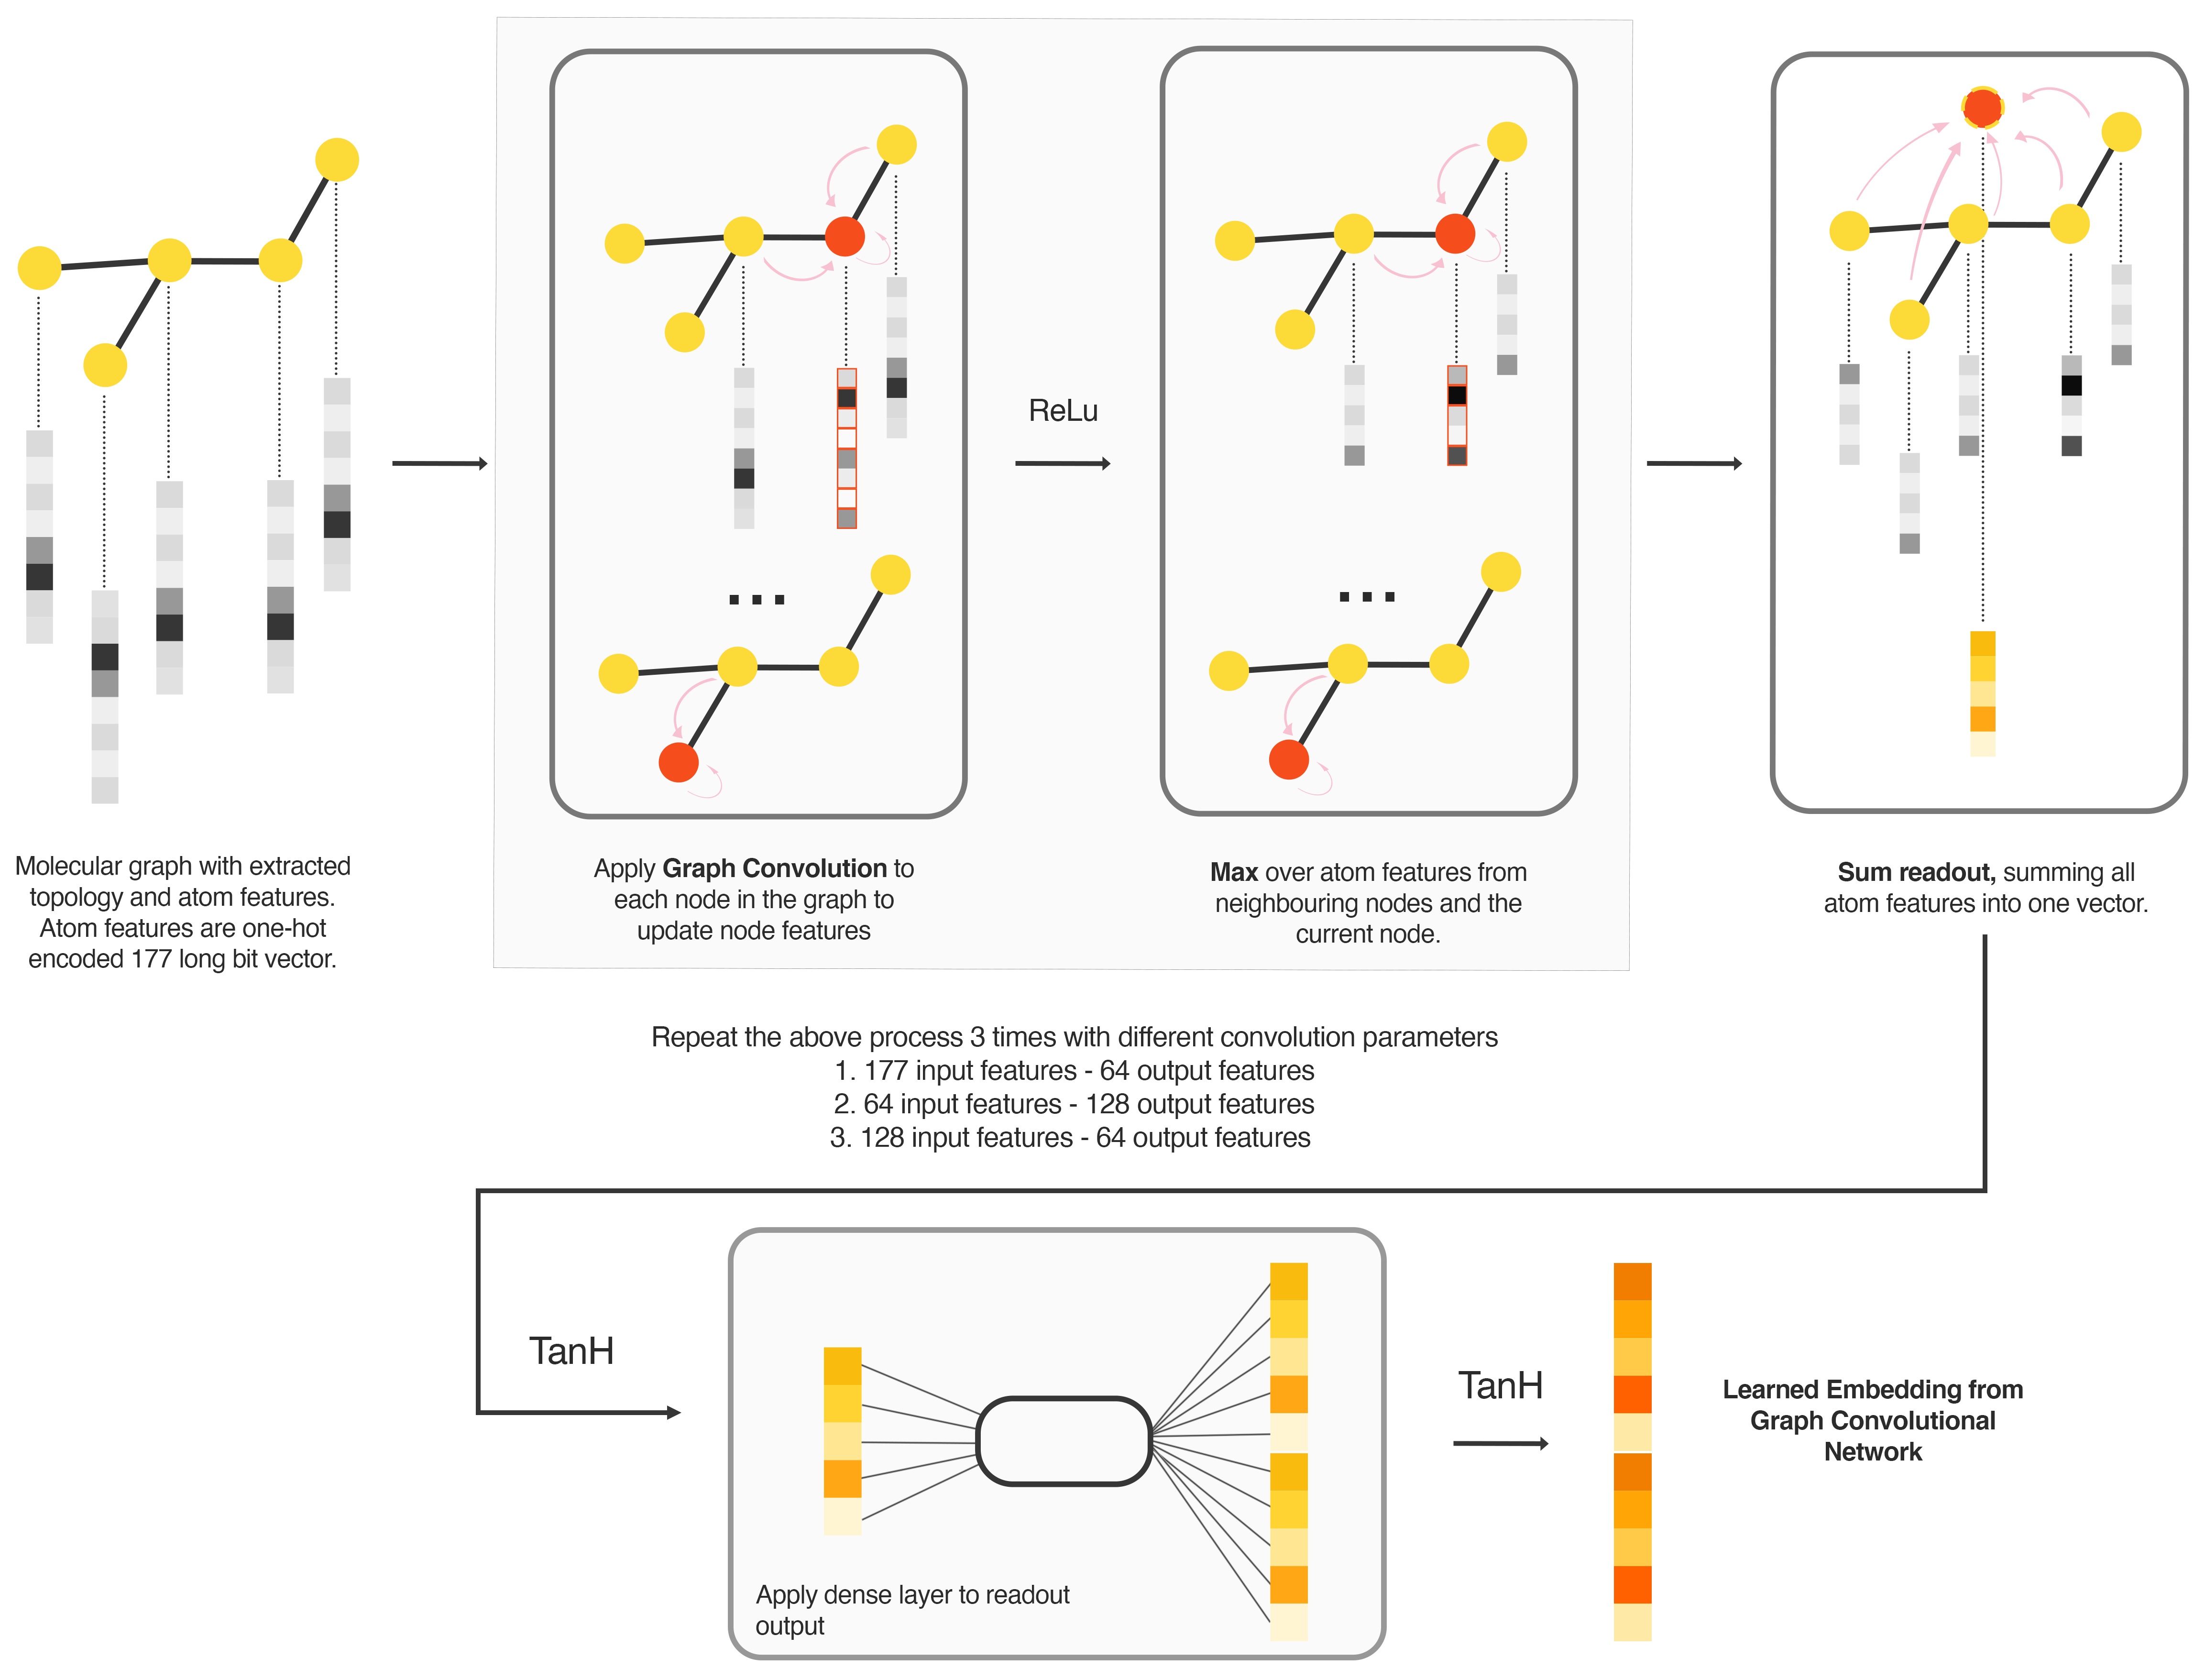
\includegraphics[width=0.75\textwidth]{img/DVGCNArchi.png}
    \caption{Learning an embedding through a Graph Convolutional Network (GCN). The molecule, represented as a graph object with nodes, edges, and atom features, is processed using graph convolutions. A max message-passing function over the current and neighbouring nodes follows each convolution layer. After this process, a sum readout aggregates all atom features into one vector. A tanh function activates this vector, and a dense linear layer processes the output vector. A non-linear tanh function activates this vector to yield the final learned molecular embedding.}
    \label{fig:dvgcnarchi}
\end{figure}

\subsubsection{Graph Convolutional Networks}

Graph convolutional networks (GCNs) are used to learn embeddings for the support and query molecules in latent space. \DIFaddbegin \DIFadd{The SMILES molecules are first converted to graph representations and later embedded as vectors in latent space using GCNs and a final dense neural network. }\DIFaddend Figure~\ref{fig:dvgcnarchi} illustrates the GCN pipeline to learn a molecular embedding. \DIFdelbegin \DIFdel{In our study , we make use of }\DIFdelend \DIFaddbegin \DIFadd{Our study uses }\DIFaddend the convolutional operator from \citet{kipf2016semi} to process graphs and learn \DIFdelbegin \DIFdel{the }\DIFdelend molecular embeddings. \DIFaddbegin \DIFadd{Back-propagation occurs throughout the whole few-shot learning process, which includes the GCNs. The assays used in testing are unseen during training. However, the molecules used in testing can be encountered during training but for different experimental assays. Since they are included in the same dataset (e.g.\ Tox21 data), these assays are related but not identical.
}\DIFaddend 

\begin{equation}
    \label{gcnequation2}
    h_i^{(l+1)} = \sigma(b^{(l)} + \sum_{j\in\mathcal{N}(i)}\frac{1}{c_{ji}}h_j^{(l)}W^{(l)})
\end{equation}

The convolutional layer can be mathematically defined through Equation~\ref{gcnequation2}. $h_j$ is the feature set of the node, $N_i$ is the set of neighbouring nodes $i$, $b$ is the learnable bias, and $c_ji$ is the product of the square root of node degrees. From a message-passing perspective, this can be summarised into the following steps for every node feature space $u$;

\begin{enumerate}
    \item Aggregating the neighbouring representations $h_v$, producing an intermediate representation $\hat{h}_u$.
    \item Transforming $\hat{h}_u$ through a linear projection and a non-linearity function such that $h_u = f(W_u \hat{h}_u)$\DIFdelbegin \DIFdel{\mbox{%DIFAUXCMD
\citep{kipf2016semi}}\hspace{0pt}%DIFAUXCMD
. }\DIFdelend \DIFaddbegin \DIFadd{. \mbox{%DIFAUXCMD
\citep{kipf2016semi}
}\hspace{0pt}%DIFAUXCMD
}\DIFaddend \end{enumerate}

Three convolutional layers are present in our architecture, after which a maximum function aggregating the node features with the maximum value of the neighbours and the node itself is applied. We highlight that this is not a coarsening operation, as the number of nodes \DIFdelbegin \DIFdel{remain }\DIFdelend \DIFaddbegin \DIFadd{remains }\DIFaddend the same. Finally, we apply a global pooling layer (readout), in which we sum over the node features of every node in the graph (see Equation~\ref{gcnequationsum}). 

\begin{equation}
    \label{gcnequationsum}
    r^{(i)} = \sum_{k=1}^{N_i} x^{(i)}_k
\end{equation}

A linear transformation is applied to the output from the readout layer, followed by a non-linear activation function, \DIFdelbegin \DIFdel{for which we use }\DIFdelend \DIFaddbegin \DIFadd{which uses }\DIFaddend a hyperbolic tangent function (tanh), outputting the final molecule embedding. Table \ref{table:gcn-architecture} contains the architecture utilised for the GCN in this study, and is illustrated in Figure~\DIFdelbegin \DIFdel{\ref{fig:dvgcnarchi2}}\DIFdelend \DIFaddbegin \DIFadd{\ref{fig:dvgcnarchi}}\DIFaddend .

\begin{table}
    \centering
    \begin{tabular}{@{}lrrl@{}}
    \hline
    \textbf{Layer Type} & \textbf{Input Dimension} & \textbf{Output Dimension} & \textbf{Non-Linearity} \\
    \hline
    GraphConv & 177 & 64 & ReLU \\
    Max Pooling & 64 & 64 & \\
    GraphConv & 64 & 128 & ReLU \\
    Max Pooling & 128 & 128 & \\
    GraphConv & 128 & 64 & ReLU \\
    Max Pooling & 64 & 64 & \\
    SumPool Readout & 64 & 64 & tanh \\
    Linear & 64 & 128 & tanh \\
    \hline  
    \end{tabular}
    \caption{Graph Convolution Network Architecture}
    \label{table:gcn-architecture}
\end{table}

\DIFdelbegin %DIFDELCMD < \begin{figure}
%DIFDELCMD < 	\centering
%DIFDELCMD < 	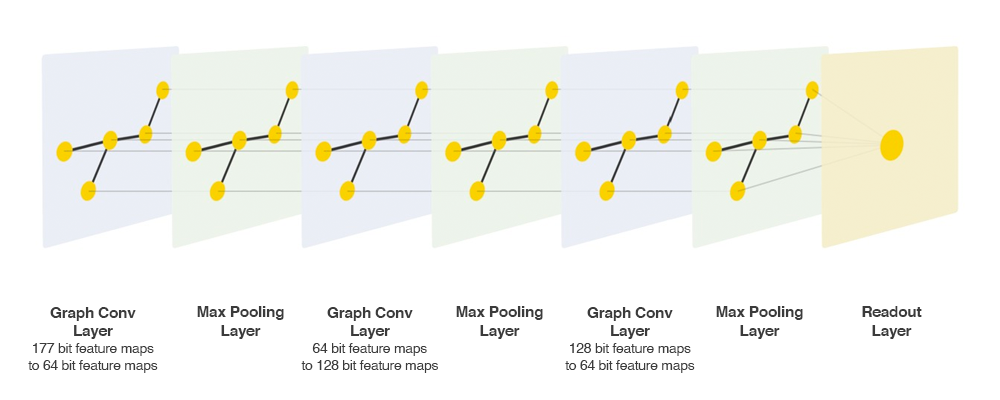
\includegraphics[width=1\linewidth]{img/gcn-layers.png}
%DIFDELCMD < 	%%%
%DIFDELCMD < \caption[Layers for graph processing in our GCN.]{%
{%DIFAUXCMD
\DIFdelFL{Graph processing layers in our GCN implementation. The graph convolution layers apply operations on each individual node's feature maps based on neighbouring nodes. The ReLU function is applied after each convolutional layer, and the tanh function is applied after the final readout layer.}}
	%DIFAUXCMD
%DIFDELCMD < \label{fig:dvgcnarchi2}
%DIFDELCMD < \end{figure}
%DIFDELCMD < 

%DIFDELCMD < %%%
\DIFdelend \subsubsection{Benchmark Models}

We \DIFdelbegin \DIFdel{make use of }\DIFdelend \DIFaddbegin \DIFadd{use }\DIFaddend a Random Forest model with 100 decision trees and a Graph Convolutional Network (GCN) to build a baseline to benchmark the purpose-built few-shot learning models. \DIFdelbegin \DIFdel{For the random forest model , }\DIFdelend \DIFaddbegin \DIFadd{The Random Forest model uses }\DIFaddend ECFP representations of the molecules of size 2,048 bits \DIFdelbegin \DIFdel{are used }\DIFdelend for the classification task, using a radius of two. Meanwhile, the same GCN architecture used for the few-shot learning models is used for our benchmark. The designated architecture for the graph convolution network is outlined in Table~\ref{table:benchmarkArchi}. The only addition to the architecture is a final linear, fully-connected layer that takes as input 128 features, which is the size of the embedding used for the experiments to follow\DIFdelbegin \DIFdel{, and }\DIFdelend \DIFaddbegin \DIFadd{. It }\DIFaddend outputs a feature of size one, onto which we apply a non-linear function, in this case\DIFaddbegin \DIFadd{, }\DIFaddend a Sigmoid function, to output the probabilities for a binary target (${0, 1}$). This binary target signifies whether the molecule belongs to the \DIFaddbegin \DIFadd{experimental assay's }\DIFaddend active or inactive/decoy class\DIFdelbegin \DIFdel{in the experimental assay}\DIFdelend . These two \DIFaddbegin \DIFadd{benchmark }\DIFaddend models are trained on a small \DIFdelbegin \DIFdel{support set, sampled from the targets assigned for testing.The remaining data for the designated target is used }\DIFdelend \DIFaddbegin \DIFadd{subset of molecules (1 to 10 molecules per class) in a particular target. The remaining molecules are used for testing, to predict the molecule's activity in the respective task. This methodology differs from the few-shot learning techniques since for the latter we reserve specific tasks (e.g.\ assays or protein targets) for training and others }\DIFaddend for testing. 

We also \DIFdelbegin \DIFdel{carry out }\DIFdelend \DIFaddbegin \DIFadd{perform }\DIFaddend a final benchmark test in retrospect by taking a random selection of query molecules from a test target, generating the ECFP with the same \DIFdelbegin \DIFdel{aforementioned parameters }\DIFdelend \DIFaddbegin \DIFadd{parameters as mentioned earlier }\DIFaddend and then calculating the Tanimoto distance to classify the remaining test molecules based on this distance. However, we find that this does not hold any significant predictive capability. 

\begin{table}
    \centering
    \begin{tabular}{@{}lrrl@{}}
    \hline
    \textbf{Layer} & \textbf{Input Dimension} & \textbf{Output Dimension} & \textbf{Non-Linearity} \\
    \hline
    GraphConv   & 177   & 64    & Relu \\
    Max Pooling & 64    & 64    &  \\
    GraphConv   & 64    & 128   & Relu \\
    Max Pooling & 64    & 64    &  \\
    GraphConv   & 128   & 64    & Relu \\
    Max Pooling & 64    & 64    &  \\
    Sum Pooling & 64    & 64    & TanH \\
    Linear      & 64    & 128   & TanH \\
    Linear      & 128   & 1     & Sigmoid \\
    \hline
    \end{tabular}
    \caption{Benchmark Neural Network for Few-Shot Learning}
    \label{table:benchmarkArchi}
\end{table}

\subsubsection{Few-Shot Learning Models}

The generated molecular embeddings from the GCN are \DIFdelbegin \DIFdel{passed to }\DIFdelend \DIFaddbegin \DIFadd{used as inputs for }\DIFaddend the few-shot learning architectures. The \DIFdelbegin \DIFdel{success of a few-shot learning model for metric-based meta-learning is dependent on the effectiveness of the kernel $k_\theta$, which measures the similarity between data samples using a metric or distance function. The }\DIFdelend models discussed in this section, excluding the benchmark model, use the embeddings generated from the GCN, \DIFdelbegin \DIFdel{presented in the }\DIFdelend \DIFaddbegin \DIFadd{grouped in }\DIFaddend support and query sets, to learn the kernel function. \DIFdelbegin %DIFDELCMD < 

%DIFDELCMD < %%%
\DIFdel{To be able to compare the model's effectiveness objectively, the GCN architecture remains unchanged in all experiments, including the benchmark.
}%DIFDELCMD < 

%DIFDELCMD < %%%
\subsubsection{\DIFdel{Siamese Networks}}
%DIFAUXCMD
\addtocounter{subsubsection}{-1}%DIFAUXCMD
%DIFDELCMD < 

%DIFDELCMD < %%%
\DIFdel{Siamese networks \mbox{%DIFAUXCMD
\citep{koch2015siamese} }\hspace{0pt}%DIFAUXCMD
are composed of two identical networks, with shared weights and parameters, taking in a pair of data samples (molecules) as inputs. The outputs from the networks are compared to learn the relationship between them. The following is the process employed for learning a classifier using Siamese Networks . The process is repeated for all training tasks.
}%DIFDELCMD < 

%DIFDELCMD < \begin{enumerate}
\begin{enumerate}%DIFAUXCMD
%DIFDELCMD <     \item %%%
\item%DIFAUXCMD
\DIFdel{Generate a list of all possible pairs between training data. If both data samples in the pair have the same target, the pair's label is set to 1, and 0 if otherwise.
    }%DIFDELCMD < \item %%%
\item%DIFAUXCMD
\DIFdel{Create a twin network using the GCN architecture to embed two molecular graph inputs into latent space.
    }%DIFDELCMD < \item %%%
\item%DIFAUXCMD
\DIFdel{Calculate the L1 distance between the molecule embeddings. This is achieved by calculating the absolute difference between the embeddings $|mol_i-mol_j|$.
    }%DIFDELCMD < \item %%%
\item%DIFAUXCMD
\DIFdel{The distance between the two embeddings is passed through a linear feedforward layer with 128 nodes and an output of 2, followed by a sigmoid function to output the probability that the two molecules belong to the same class. }%DIFDELCMD < \item %%%
\item%DIFAUXCMD
\DIFdel{As we are dealing with binary classification, the binary cross-entropy loss is calculated and backpropagated to the network.
}
\end{enumerate}%DIFAUXCMD
%DIFDELCMD < \end{enumerate}
%DIFDELCMD < 

%DIFDELCMD < %%%
\subsubsection{\DIFdel{Matching Networks}}
%DIFAUXCMD
\addtocounter{subsubsection}{-1}%DIFAUXCMD
%DIFDELCMD < 

%DIFDELCMD < %%%
\DIFdel{Matching Networks extends Siamese Networks, but instead of learning a metric function over pairs of data, the classifier learns how to define a probability distribution of output labels from query/test examples using a support set $S$. The classifier outputs a sum of attention-weighted labels from the support set to predict the similarity between the test example and the samples from the support set. We use the same embedding function for the support and query sets to compute the molecular embeddings. Subsequently, the cosine similarity of pairs of data points between the support and query sets is computed, which is then normalised by a softmax function. As proposed in \mbox{%DIFAUXCMD
\citet{vinyals2016matching}}\hspace{0pt}%DIFAUXCMD
, Fully Contextual Embeddings (FCE) are used in our implementation. Taking single data points to learn an embedding function limits the ability of embedding the molecules effectively into latent space. Therefore, a bidirectional long-short term memory (LSTM) is used , taking as input the whole support set to adjust the embedding based on the other support samples.
}%DIFDELCMD < 

%DIFDELCMD < %%%
\DIFdel{Two functions are defined. $g_\theta(x_i, S)$ encodes $x_i$, a data sample from the support set, in the context of the whole support set $S$, using a bidirectional LSTM. The LSTM transforms our support set embeddings by adding the forward and backward activations to the original support image embeddings. Subsequently, $f_\theta(x, S)$, encodes the query sample $x$ and trains the LSTM with read attention over the support set. The hidden state is updated over ten processing ``read'' steps, until eventually the hidden state is equivalent to the aforementioned $f_\theta(x, S)$. Throughout each iteration, the hidden state and the output from the attention function are added together. To train the network using stochastic gradient descent, the cross-entropy loss is computed for each query prediction.
}%DIFDELCMD < 

%DIFDELCMD < %%%
\subsubsection{\DIFdel{Prototypical Networks}}
%DIFAUXCMD
\addtocounter{subsubsection}{-1}%DIFAUXCMD
%DIFDELCMD < 

%DIFDELCMD < %%%
\DIFdel{Prototypical Networks \mbox{%DIFAUXCMD
\citep{snell2017prototypical} }\hspace{0pt}%DIFAUXCMD
have similarities to the Matching Networks described above, but instead of considering the individual support set embeddings, the mean vector of the embeddings for each class within the support set is taken. This mean vector for each class is referred to as the }\textit{\DIFdel{prototype}}%DIFAUXCMD
\DIFdel{. Another improvement the authors make over Matching Networks, is the use of Euclidean rather than the cosine distance. In order to classify query data samples, the softmax of the inverse of the euclidean distances between each query and each prototype is taken. To train the network through stochastic gradient descent, the negative log-likelihood loss is used. }%DIFDELCMD < 

%DIFDELCMD < %%%
\subsubsection{\DIFdel{Relation Networks}}
%DIFAUXCMD
\addtocounter{subsubsection}{-1}%DIFAUXCMD
%DIFDELCMD < 

%DIFDELCMD < %%%
\DIFdel{For the Relation Networks \mbox{%DIFAUXCMD
\citep{sung2018learning}}\hspace{0pt}%DIFAUXCMD
, the classification of query samples is not done directly in latent space from the embeddings. The embeddings for the support and query samples are generated using the GCN. Following this step, the feature maps concatenations are created by concatenating the query samples with each data sample within the support set. The feature map concatenation therefore is double the length of the embedding generated by the GCN}\DIFdelend \DIFaddbegin \DIFadd{These models include Siamese Networks, Matching Networks, Prototypical Networks and Relation Networks. Table \ref{table:relation-neural-net} tabulates the network used to generate the relation score in the Relation Networks architecture. The GCN architecture remains unchanged in all experiments to compare the model's effectiveness objectively. Figure~\ref{fig:schematic-training} illustrates the rationale behind few-shot machine learning for this problem domain. The molecules used in training and testing can be shared; however, the target class information imparting activity in a specific experimental assay must be different. This separation entails that we present the machine learning model with information from previously unseen experimental assays during testing. For example, training can be done on molecular activity for nuclear receptor assays in Tox21 and then tested on the remaining assays, which would have never been seen during training}\DIFaddend .

\DIFdelbegin \DIFdel{The relationship between the queries and the different classes within the support set is captured by passing these feature map concatenations through a feed forward neural network $g_\theta([x_i, x_j])$ to predict a relation score. $[\cdot,\cdot]$ is the concatenation between each support set data sample $x_i$ and the query data samples $x_j$. The architecture of this function is defined in Table~\ref{table:relation-neural-net}. The loss function used is Mean Squared Error (MSE) loss as proposed in the original paper.
}\DIFdelend \DIFaddbegin \begin{figure}[ht!]
    \centering
    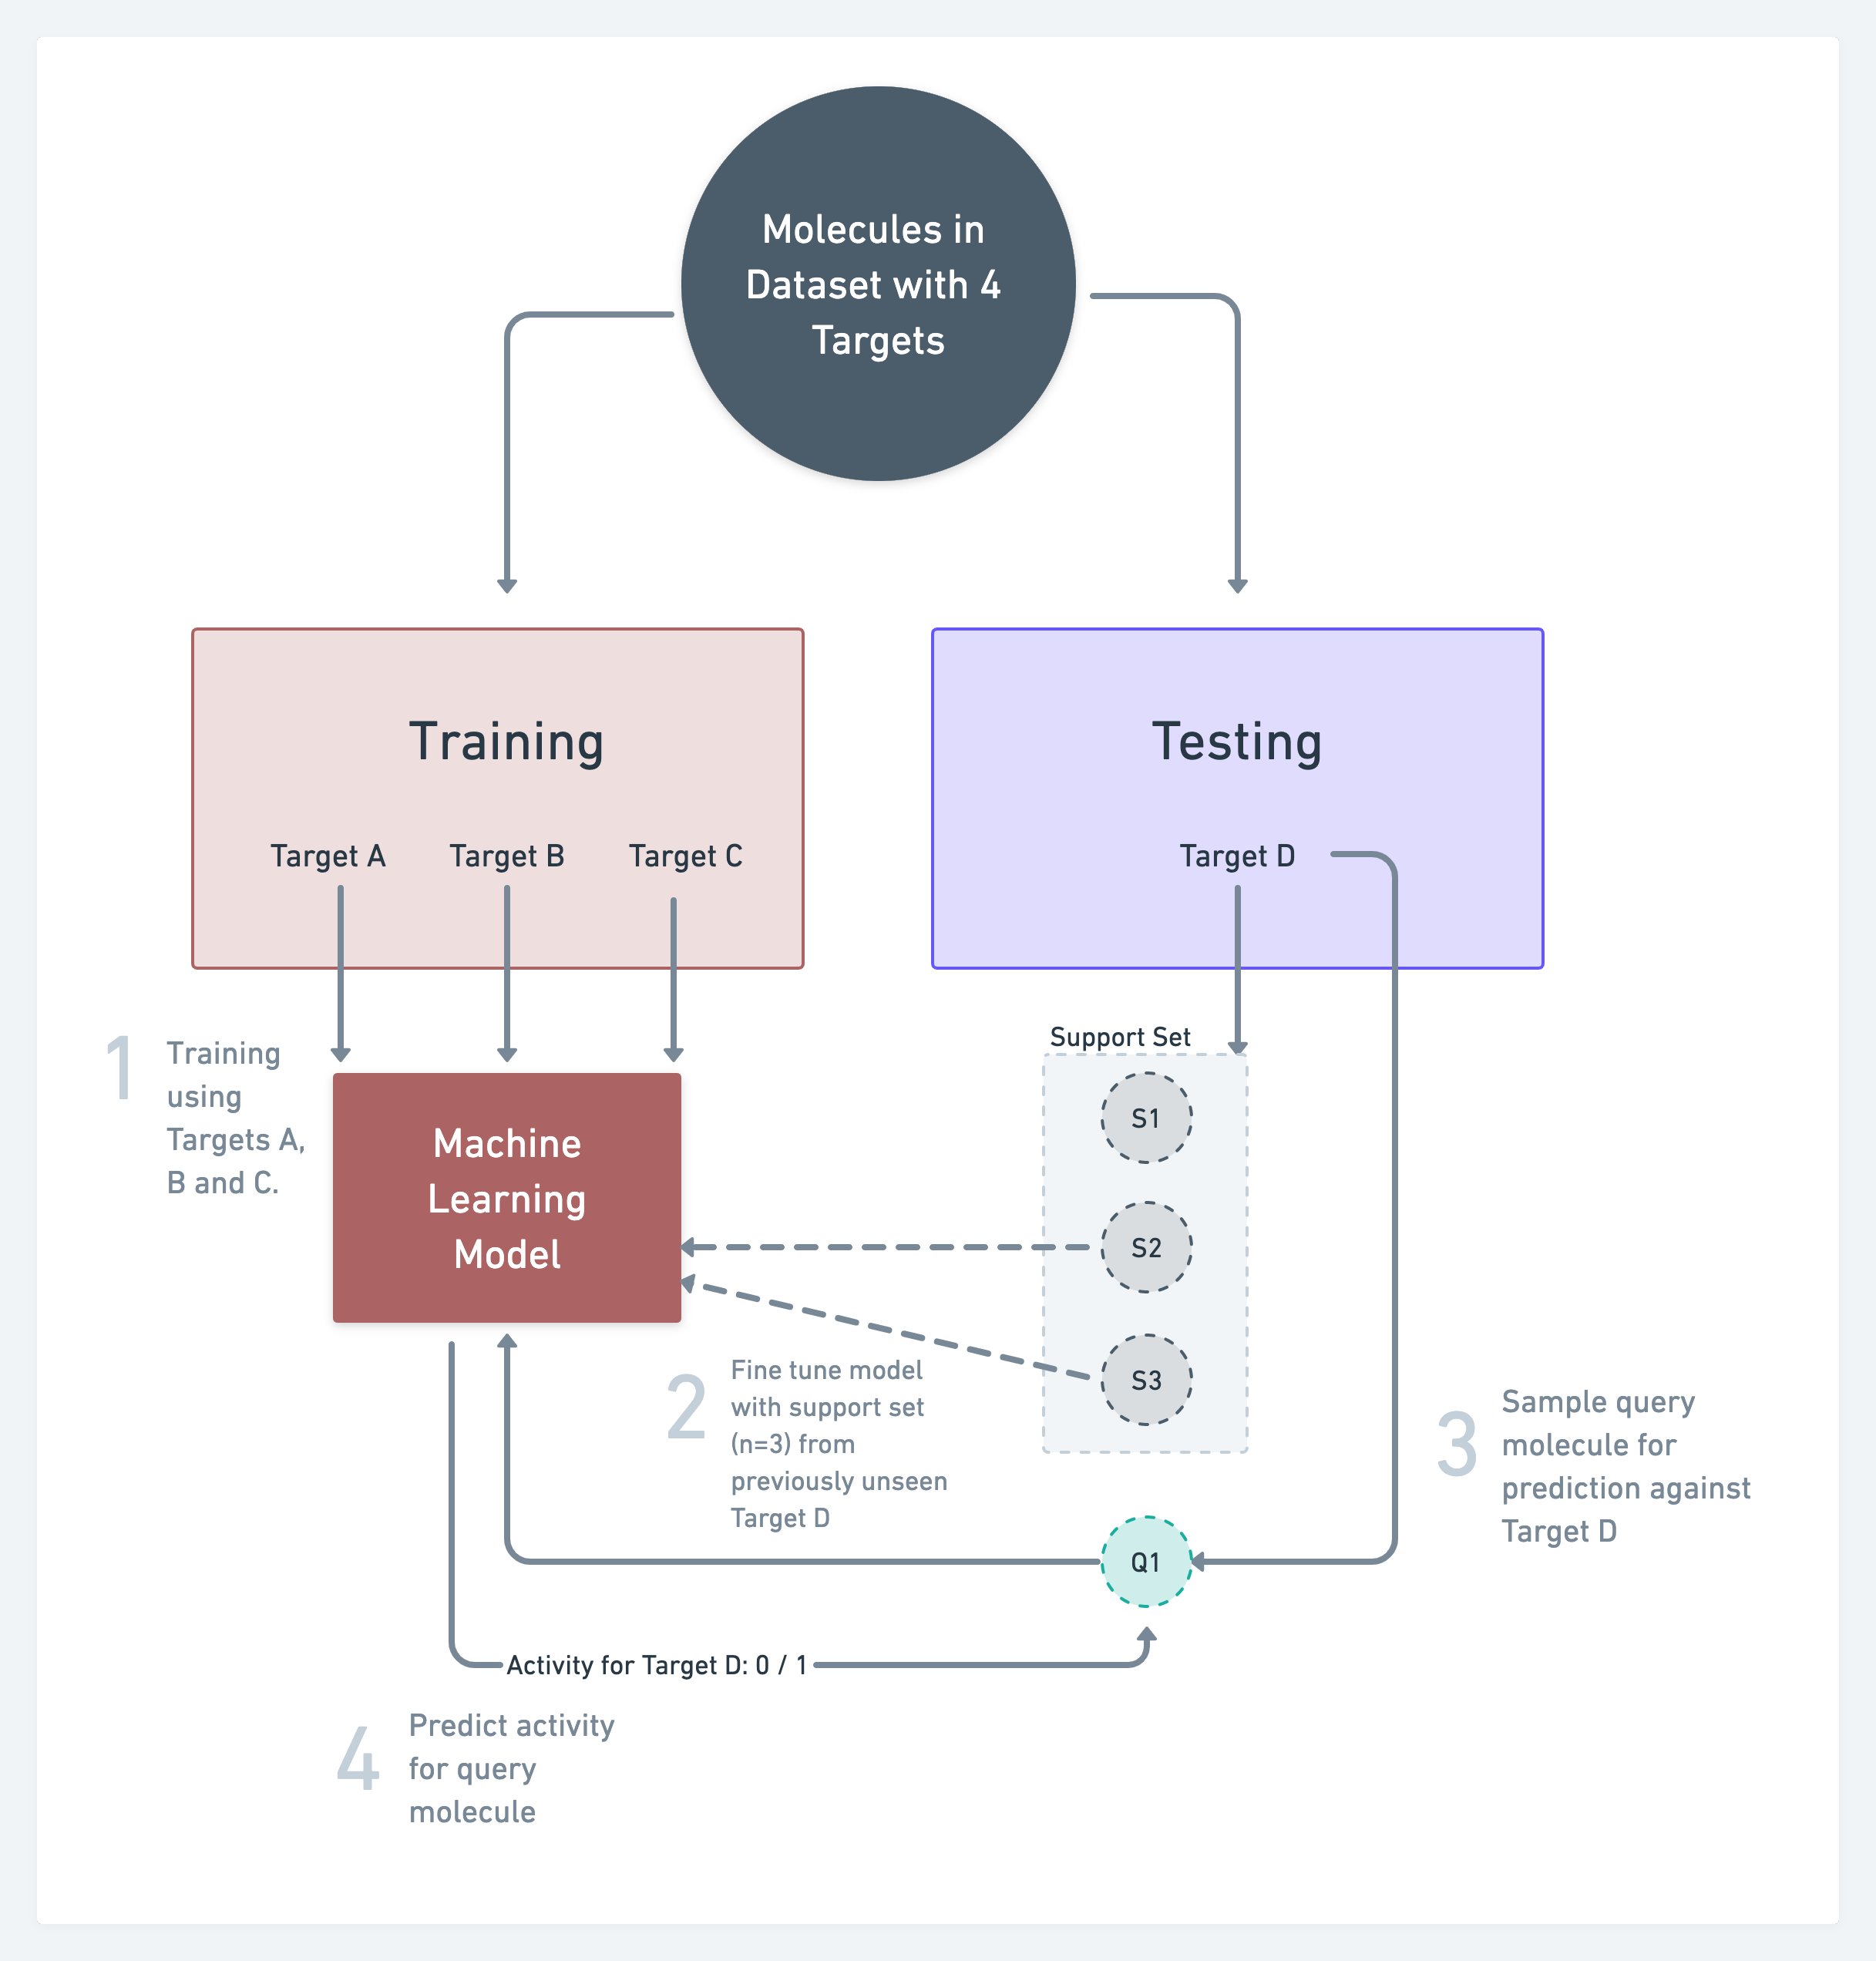
\includegraphics[width=0.75\textwidth]{img/Schematic Training.png}
    \caption{\DIFaddFL{Schematic illustrating how the few-shot learning machine learning on a molecular dataset works. The same molecules can be used during training and testing; however, these molecules would impart different information based on the target or experimental assay. The targets used in testing are previously unseen, except for the few molecules sampled in the support set (S\textsubscript{1-3}), which are used to fine-tune the ML model and impart some information about Target D. Query molecule Q\textsubscript{1} is sampled from Target D to be predicted using the ML model.}}
    \label{fig:schematic-training}
\end{figure}
\DIFaddend 

\begin{table*}[h]
    \centering
    \begin{tabular}{@{}lrrl@{}}
    \hline
    Layer Type & Input Dimension & Output Dimension & Non-Linearity \\
    \hline
    Linear  & 256   & 128   & ReLU \\
    Linear  & 128   & 64    & ReLU \\
    Linear  & 64    & 8     & ReLU \\
    Linear  & 8     & 2     & Sigmoid \\
    \hline
    \end{tabular}
    \caption{The architecture for generating the relation score using function $g_\theta$.}
    \label{table:relation-neural-net}
\end{table*}

We \DIFdelbegin \DIFdel{sample a total of 128 query molecules for each episode, which is composed of a balanced combination of molecules from each class. If the active class for a specific target contains less than 64 molecules, the active molecules are over-sampled such that each query set contains 64 actives. We }\DIFdelend reproduce the work of \citet{altae2017low} from scratch and \DIFdelbegin \DIFdel{also }\DIFdelend apply the IterRefLSTM to the embeddings \DIFdelbegin \DIFdel{from all other networks }\DIFdelend \DIFaddbegin \DIFadd{in all architectures }\DIFaddend to effectively compare our contribution to past work. Additionally, we also provide implementations for the Prototypical Networks and Relation Networks. All the experiments are run on Google Colaboratory\DIFaddbegin \DIFadd{, }\DIFaddend and all implementations are open-sourced on GitHub\footnote{Accessed From: \url{https://github.com/danielvlla/Few-Shot-Learning-for-Low-Data-Drug-Discovery}}. As emphasised by \citet{vinyals2016matching} and \citet{snell2017prototypical}, training and testing conditions should match \DIFdelbegin \DIFdel{when doing }\DIFdelend \DIFaddbegin \DIFadd{during }\DIFaddend few-shot learning. Therefore, the \DIFdelbegin \DIFdel{same support set composition used }\DIFdelend \DIFaddbegin \DIFadd{exact same number of actives and inactives/decoys that make up the support set }\DIFaddend to train the model is \DIFdelbegin \DIFdel{used during test time}\DIFdelend \DIFaddbegin \DIFadd{also used during testing}\DIFaddend . For example, if we train using 10-shot learning, testing is carried out with 10-shot support sets. We remind the reader that testing is carried out on a new, previously unseen target. After the support set has been sampled, the rest of the data for the target being tested is used as query data. This process is repeated 20 times, and the mean and standard deviation of the ROC-AUC and PR-AUC scores from these 20 rounds are reported as the final classification result.

\subsubsection{Evaluation}

The evaluation metrics \DIFdelbegin \DIFdel{used }\DIFdelend \DIFaddbegin \DIFadd{we use }\DIFaddend are the Area Under Curve (AUC) of the Receiver Operating Characteristic (ROC) curve \DIFdelbegin \DIFdel{, }\DIFdelend and the Precision-Recall Curve (PR-AUC). To determine \DIFdelbegin \DIFdel{the predictive power of our classifier, we make use of }\DIFdelend \DIFaddbegin \DIFadd{our classifier's predictive power, we use }\DIFaddend the ROC Area Under Curve (AUC) (ROC-AUC) as this \DIFdelbegin \DIFdel{provides a clearer picture of the relationship between the true positive and the false positive rate. The ROC-AUC }\DIFdelend affords a more nuanced approach than \DIFdelbegin \DIFdel{accuracy as it provides }\DIFdelend \DIFaddbegin \DIFadd{the accuracy metric, providing }\DIFaddend visibility into thresholds one can utilise to ameliorate predictions. \citet{altae2017low} \DIFdelbegin \DIFdel{only }\DIFdelend \DIFaddbegin \DIFadd{also }\DIFaddend report ROC-AUC results\DIFdelbegin \DIFdel{, however, }\DIFdelend \DIFaddbegin \DIFadd{; however, we believe }\DIFaddend this metric alone does not adequately measure the \DIFdelbegin \DIFdel{nature of the }\DIFdelend performance of the machine learning models due to the highly imbalanced nature of the data at hand. In virtual screening, \DIFdelbegin \DIFdel{the detection of }\DIFdelend \DIFaddbegin \DIFadd{detecting }\DIFaddend rare events (equivalent to our minority active class) holds significant importance, as active compounds against a specific target should be identified from the compound database. However, we do not disregard the importance of correct classification of the majority inactive/decoy class, as this is also important for filtering out thousands of screened compounds. As the active class is the minority class, PR-AUC is used to evaluate how well the model can classify the active class\DIFaddbegin \DIFadd{.
}\DIFaddend 

We apply statistical analysis \DIFdelbegin \DIFdel{on }\DIFdelend \DIFaddbegin \DIFadd{to }\DIFaddend the ROC-AUC and PR-AUC scores from the 20 test rounds for each experiment to establish whether there are significant differences between the few-shot learning models. The scores are compared against \DIFdelbegin \DIFdel{those of }\DIFdelend \DIFaddbegin \DIFadd{the scores from }\DIFaddend the model that obtained the best result for the same conditions. Comparison of results between two models is carried out using the Mann-Whitney U-test, also referred to as the Wilcoxon rank sum test \citep{mann1947test}.

\section{Implementation Details}

\DIFdelbegin \DIFdel{These }\DIFdelend \DIFaddbegin \DIFadd{The machine learning }\DIFaddend models were developed using Python 3.7. Most packages were installed using Pip 21.0.1\DIFdelbegin \DIFdel{, }\DIFdelend \DIFaddbegin \DIFadd{; }\DIFaddend however, Conda 4.10.3 was also used to install packages not found on the Python Package Index (PyPi)\footnote{Accessed from: \url{https://pypi.org/}. Last Accessed: 26/\DIFdelbegin \DIFdel{05}\DIFdelend \DIFaddbegin \DIFadd{09}\DIFaddend /2022}. Pip and conda are package management systems for Python, allowing users to \DIFdelbegin \DIFdel{conveniently }\DIFdelend install and run packages and their dependencies \DIFaddbegin \DIFadd{conveniently}\DIFaddend . The specific versions of each toolkit are specified in Table~\ref{tab:versions}.

\begin{table}
    \centering
    \begin{tabular}{@{}lll@{}}
        \hline
        \textbf{Package} & \textbf{Version} & \textbf{Description} \\
        \hline
        PyTorch & 1.9.0 & Machine learning framework \\
        Scikit-Learn & 1.0.1 & Machine Learning Library \\
        Deep Graph Library (DGL) & 0.7.2 & Deep learning on graphs \\
        DGL-LifeSci & 0.2.8 & Cheminformatics graph functions \\
        RDKit & 2021.09.2 & Cheminformatics Toolkit \\
        DeepChem & 2.6.0.dev & Cheminformatics Machine Learning \\
        Pandas & 1.1.5 & Data manipulation and preparation \\
        Numpy & 1.19.5 & Adds support for multi-dimensional arrays \\
        ChemBL Structure Pipeline & 1.0.0 & Used to standardise molecules \\
        NetworkX & 2.6.3 & Used to visualise graphs \\
        TQDM & 4.59 & Progress bars library \\
        SciPy & 1.7.1 & Statistical Analysis \\
        \hline
    \end{tabular}
    \caption{Python libraries utilised for this project.}
    \label{tab:versions}
\end{table}

All the experiments were run on Google Colaboratory\footnote{Accessed from: \url{https://colab.research.google.com/}. Last Accessed: 26/\DIFdelbegin \DIFdel{05}\DIFdelend \DIFaddbegin \DIFadd{09}\DIFaddend /2022}, Colab in short\DIFdelbegin \DIFdel{. Colab is a hosted Jupyter notebook}\footnote{\DIFdel{Accessed from: }%DIFDELCMD < \url{https://jupyter.org/}%%%
\DIFdel{. Last Accessed: 26/05/2022}} %DIFAUXCMD
\addtocounter{footnote}{-1}%DIFAUXCMD
\DIFdel{service, providing access to computational resources including CPUs and GPUs to run Python code. These Colab notebooks can be shared, accessed, and run in web-browsers.  The Colab instance }\DIFdelend \DIFaddbegin \DIFadd{, and this platform's }\DIFaddend details are specified in Table~\ref{tab:hardware}.

\begin{table}
    \centering
    \begin{tabular}{@{}lll@{}}
        \hline
        \textbf{Type} & \textbf{Model} & \textbf{Details} \\
        \hline
        CPU & Intel (R) Xeon & 2.20~Ghz 4 Cores \\
        GPU & Nvidia Tesla P100 & 16~GB using Cuda 11.1 \\
        RAM & N/A & 25~GB \\
        \hline
    \end{tabular}
    \caption{Hardware provisioned in Google Colab.}
    \label{tab:hardware}
\end{table}

\section{Results}

\DIFdelbegin \DIFdel{In this section we present }\DIFdelend \DIFaddbegin \DIFadd{This section presents }\DIFaddend the few-shot model results for the three evaluation datasets, Tox21, MUV, and DUD-E. All \DIFdelbegin \DIFdel{these }\DIFdelend \DIFaddbegin \DIFadd{three }\DIFaddend datasets are highly imbalanced, where the inactive/\DIFdelbegin \DIFdel{decoys }\DIFdelend \DIFaddbegin \DIFadd{decoy molecules }\DIFaddend greatly outnumber the number of actives. This \DIFdelbegin \DIFdel{defining feature of these datasets }\DIFdelend \DIFaddbegin \DIFadd{imbalance }\DIFaddend presents a challenging problem \DIFdelbegin \DIFdel{, but is also further evidence }\DIFdelend \DIFaddbegin \DIFadd{but proves }\DIFaddend that low-data machine learning is highly beneficial in this domain. We first present the work we reproduced from \citet{altae2017low}, which we also \DIFaddbegin \DIFadd{use to }\DIFaddend test on a subset of the DUD-E dataset. \DIFdelbegin \DIFdel{This was not explored in the original study. }\DIFdelend The reproduced work includes Siamese Networks \citep{koch2015siamese} and the Matching Networks \citep{vinyals2016matching} with the \DIFdelbegin \DIFdel{Iterative Refinement LSTM (IterRefLSTM)}\DIFdelend \DIFaddbegin \DIFadd{IterRefLSTM}\DIFaddend . The latter obtained the best results in \citet{altae2017low} \DIFdelbegin \DIFdel{. This is followed by the presentation and discussion of the }\DIFdelend \DIFaddbegin \DIFadd{and is referred to as the state-of-the-art in this study. Further building on the Matching Networks architecture by \mbox{%DIFAUXCMD
\citet{vinyals2016matching}}\hspace{0pt}%DIFAUXCMD
, we present and discuss }\DIFaddend results for two newly proposed machine learning models in this domain\DIFdelbegin \DIFdel{, which are based on work of \mbox{%DIFAUXCMD
\citet{vinyals2016matching} }\hspace{0pt}%DIFAUXCMD
for Matching Networks}\DIFdelend . These machine learning models include the Prototypical \citep{snell2017prototypical} and Relation \citep{sung2018learning} Networks. \DIFaddbegin \DIFadd{These architectures have been previously explored for the computer vision domain but, to our knowledge, have never been applied to the drug discovery domain. }\DIFaddend Finally, we evaluate the results with the \DIFdelbegin \DIFdel{state of the art}\DIFdelend \DIFaddbegin \DIFadd{state-of-the-art}\DIFaddend , which is identified to be the work of \citet{altae2017low}.


\subsection{Tox21}

In line with the results reported by \citet{altae2017low}, the few-shot learning models on Tox21 outperform the benchmark models significantly. The Matching Networks with IterRefLSTM performs well and obtain the best ROC-AUC results in \DIFdelbegin \DIFdel{a number of experiments. The fact that the same implementation for the Matching Networks (MNs) obtained slightly better results (1-14\% across the five support set experiments) than the state-of-the-art work, can be attributed to the set of atom descriptors used for the initial graph representations presented earlier}\DIFdelend \DIFaddbegin \DIFadd{some experiments}\DIFaddend . Our few-shot learning architecture implementation is identical to the work of \citet{altae2017low}\DIFdelbegin \DIFdel{, however}\DIFdelend \DIFaddbegin \DIFadd{; however, slight }\DIFaddend variations in how the model learns could be present. Hence, we focus mainly on \DIFdelbegin \DIFdel{the performance of }\DIFdelend how our implementations performed against each other. The results from the Prototypical Networks (PNs) overall \DIFaddbegin \DIFadd{significantly }\DIFaddend outperform the results from the MNs \DIFaddbegin \DIFadd{(the state-of-the-art approach) }\DIFaddend based on statistical analysis (see Table~\ref{table:Tox21-mean}). Meanwhile, MNs and PNs, \DIFdelbegin \DIFdel{overall }\DIFdelend outperform Relation Networks (RNs) in both ROC-AUC and PR-AUC performance. 

Results for \DIFdelbegin \DIFdel{one shot-learning }\DIFdelend \DIFaddbegin \DIFadd{one-shot learning }\DIFaddend do not provide a clear-cut choice between our implementations for MNs and PNs with the IterRefLSTM\DIFdelbegin \DIFdel{, which }\DIFdelend \DIFaddbegin \DIFadd{. This performance }\DIFaddend is expected due to the \DIFaddbegin \DIFadd{similarity in the }\DIFaddend architecture of these methods. In a one-shot learning scenario, MNs and PNs are conceptually similar. The main difference lies in the distance function used \DIFdelbegin \DIFdel{as }\DIFdelend \DIFaddbegin \DIFadd{since }\DIFaddend for MNs we use the cosine distance, while for PNs, we \DIFdelbegin \DIFdel{make use of the euclidean }\DIFdelend \DIFaddbegin \DIFadd{use the Euclidean }\DIFaddend distance, as proposed in the original literature\DIFaddbegin \DIFadd{, }\DIFaddend which introduced these two techniques. They both achieve comparable performance on Tox21 targets for one-shot learning. The performance of MNs for this scenario is consistent with the state-of-the-art \DIFdelbegin \DIFdel{work }\DIFdelend and for such a \DIFdelbegin \DIFdel{difficult }\DIFdelend \DIFaddbegin \DIFadd{problematic }\DIFaddend scenario (i.e.\ learning with only one example from each class), results are promising. The \textit{prototypes} in PNs are a mean of all embeddings for each class in the support set. The \DIFdelbegin \DIFdel{euclidean distance between the }\DIFdelend \DIFaddbegin \DIFadd{Euclidean distance between }\DIFaddend \textit{prototypes} and each embedding from the query set is calculated to predict the query's activity. As in one-shot learning we only have one example per class, the \textit{prototypes} are equivalent to the embedding for each class, making this identical to the MNs. 

\DIFaddbegin \DIFadd{One observation which can be made is that there is not a significant improvement in performance from one-shot learning to 10-shot learning. This consistency may be attributed to the methodology used for training. Few-shot learning conditions during training must match the ones during testing, but during training, we use a sequence of episodes, in which we match the few-shot conditions during testing in each episode. Having a sequence of episodes means that training sees many molecules, albeit in a few-shot scenario. Hence, the model itself may already be maximally informative due to the number of episodes it is exposed to. Thus, when we get to the testing stage, presenting one-shot or 10-shot support sets to fine-tune the model does not seem to make an impactful difference. Another possible explanation for the insignificant impact of the support sets size on the performance of the few-shot learning models is that there is an inherent bias across targets in the dataset which the methods are able to pick upon. If this is the case, it would warrant future research on the composition of the Tox21 dataset when used to evaluate Machine Learning models. 
}

\DIFaddend \begin{table}
    \caption{Mean ROC-AUC and PR-AUC Scores with standard deviation for ML Models for the Tox21 Test Targets over 20 rounds of testing. \DIFdelbeginFL \DIFdelFL{Bold }\DIFdelendFL \DIFaddbeginFL \DIFaddFL{The bold }\DIFaddendFL text illustrates the \DIFdelbeginFL \DIFdelFL{best obtained }\DIFdelendFL \DIFaddbeginFL \DIFaddFL{best-obtained }\DIFaddendFL value. The first column shows the composition of the support set. The reproduced results \DIFdelbeginFL \DIFdelFL{from }\DIFdelendFL \DIFaddbeginFL \DIFaddFL{use our implementation of }\DIFaddendFL the \DIFdelbeginFL \DIFdelFL{model used }\DIFdelendFL \DIFaddbeginFL \DIFaddFL{MatchingNet architecture }\DIFaddendFL in \citet{altae2017low}\DIFdelbeginFL \DIFdelFL{is the MatchingNet}\DIFdelendFL . The actual values are tabulated in the supporting information document in \DIFdelbeginFL \DIFdelFL{tables }\DIFdelendFL \DIFaddbeginFL \DIFaddFL{Tables }\DIFaddendFL S1, S2, and S3.}
    \centering
    % \ra{1.3}
    % {\renewcommand{\arraystretch}{1}}
    \DIFdelbeginFL %DIFDELCMD < \resizebox{\textwidth}{!}{%
%DIFDELCMD < 		\begin{tabular}{@{}cccccccc@{}}
%DIFDELCMD < 			\hline
%DIFDELCMD < 			\textbf{Tox21} & \textbf{Metric} & \textbf{RF} & \textbf{Graph Conv} & \textbf{SiameseNet} & \textbf{MatchingNet} & \textbf{ProtoNet} & \textbf{RelationNet} \\
%DIFDELCMD < 			\hline
%DIFDELCMD < 			10+/10- & ROC-AUC & 0.617 ± 0.060 & 0.620 ± 0.065 & 0.825 ± 0.043 & 0.824 ± 0.022 & \textbf{0.826 ± 0.034} & 0.814 ± 0.030 \\ & PR-AUC & 0.158 ± 0.102 & 0.150 ± 0.095 & 0.226 ± 0.107 & 0.367 ± 0.105 & \textbf{0.384 ± 0.105} & 0.360 ± 0.102\\
%DIFDELCMD < 			\hline
%DIFDELCMD < 			5+/10- & ROC-AUC & 0.602 ± 0.059 & 0.610 ± 0.062 & 0.828 ± 0.069 & \textbf{0.824 ± 0.033} & 0.823 ± 0.038 & 0.822 ± 0.023 \\ & PR-AUC & 0.148 ± 0.090 & 0.152 ± 0.094 & 0.190 ± 0.094 & 0.369 ± 0.110 & \textbf{0.388 ± 0.111} & 0.355 ± 0.104\\
%DIFDELCMD < 			\hline
%DIFDELCMD < 			1+/10- & ROC-AUC & 0.563 ± 0.068 & 0.558 ± 0.076 & 0.836 ± 0.138 & 0.822 ± 0.025 & \textbf{0.826 ± 0.032} & 0.814 ± 0.028 \\ & PR-AUC & 0.128 ± 0.084 & 0.126 ± 0.075 & 0.099 ± 0.093 & 0.301 ± 0.103 & \textbf{0.384 ± 0.096} & 0.325 ± 0.103\\
%DIFDELCMD < 			\hline
%DIFDELCMD < 			1+/5- & ROC-AUC & 0.534 ± 0.066 & 0.559 ± 0.090 & 0.807 ± 0.159 & \textbf{0.820 ± 0.033} & \textbf{0.820 ± 0.033} & 0.819 ± 0.023 \\ & PR-AUC & 0.112 ± 0.059 & 0.128 ± 0.080 & 0.106 ± 0.086 & 0.339 ± 0.115 & \textbf{0.362 ± 0.106} & 0.318 ± 0.108\\
%DIFDELCMD < 			\hline
%DIFDELCMD < 			1+/1- & ROC-AUC & 0.550 ± 0.061 & 0.548 ± 0.102 & 0.818 ± 0.075 & 0.819 ± 0.036 & \textbf{0.820 ± 0.030} & 0.813 ± 0.029 \\ & PR-AUC & 0.118 ± 0.068 & 0.123 ± 0.082 & 0.198 ± 0.102 & 0.352 ± 0.121 & \textbf{0.373 ± 0.102} & 0.342 ± 0.093\\
%DIFDELCMD < 			\hline
%DIFDELCMD < 		\end{tabular}
%DIFDELCMD < 	}
%DIFDELCMD < 	%%%
\DIFdelendFL \DIFaddbeginFL \resizebox{\textwidth}{!}{%
        \begin{tabular}{@{}cccccccc@{}}
            \hline
            \textbf{Tox21} & \textbf{Metric} & \textbf{RF} & \textbf{Graph Conv} & \textbf{SiameseNet} & \textbf{MatchingNet} & \textbf{ProtoNet} & \textbf{RelationNet} \\
            \hline
            10+/10- & ROC-AUC & 0.617 ± 0.060 & 0.620 ± 0.065 & 0.825 ± 0.043 & 0.824 ± 0.022 & \textbf{0.826 ± 0.034} & 0.814 ± 0.030 \\ & PR-AUC & 0.158 ± 0.102 & 0.150 ± 0.095 & 0.226 ± 0.107 & 0.367 ± 0.105 & \textbf{0.384 ± 0.105} & 0.360 ± 0.102\\
            \hline
            5+/10- & ROC-AUC & 0.602 ± 0.059 & 0.610 ± 0.062 & 0.828 ± 0.069 & \textbf{0.824 ± 0.033} & 0.823 ± 0.038 & 0.822 ± 0.023 \\ & PR-AUC & 0.148 ± 0.090 & 0.152 ± 0.094 & 0.190 ± 0.094 & 0.369 ± 0.110 & \textbf{0.388 ± 0.111} & 0.355 ± 0.104\\
            \hline
            1+/10- & ROC-AUC & 0.563 ± 0.068 & 0.558 ± 0.076 & \textbf{0.836 ± 0.138} & 0.822 ± 0.025 & 0.826 ± 0.032 & 0.814 ± 0.028 \\ & PR-AUC & 0.128 ± 0.084 & 0.126 ± 0.075 & 0.099 ± 0.093 & 0.301 ± 0.103 & \textbf{0.384 ± 0.096} & 0.325 ± 0.103\\
            \hline
            1+/5- & ROC-AUC & 0.534 ± 0.066 & 0.559 ± 0.090 & 0.807 ± 0.159 & \textbf{0.820 ± 0.033} & \textbf{0.820 ± 0.033} & 0.819 ± 0.023 \\ & PR-AUC & 0.112 ± 0.059 & 0.128 ± 0.080 & 0.106 ± 0.086 & 0.339 ± 0.115 & \textbf{0.362 ± 0.106} & 0.318 ± 0.108\\
            \hline
            1+/1- & ROC-AUC & 0.550 ± 0.061 & 0.548 ± 0.102 & 0.818 ± 0.075 & 0.819 ± 0.036 & \textbf{0.820 ± 0.030} & 0.813 ± 0.029 \\ & PR-AUC & 0.118 ± 0.068 & 0.123 ± 0.082 & 0.198 ± 0.102 & 0.352 ± 0.121 & \textbf{0.373 ± 0.102} & 0.342 ± 0.093\\
            \hline
        \end{tabular}
    }
    \DIFaddendFL \label{table:Tox21-mean}
\end{table}

\subsection{MUV}

Each active in the MUV dataset is structurally distinct from the other, making each data sample maximally informative. Therefore, structural similarities cannot be exploited on unseen active molecules. \DIFaddbegin \DIFadd{Our results show that the few-shot learning techniques explored in this study are better suited for lead optimisation (such as toxicity information) rather than hit discovery, for which MUV is mostly designed. }\DIFaddend The baseline benchmark tests consistently outperformed few-shot learning techniques. \citet{altae2017low} report that the results obtained through the GCNs baseline also struggle in performance\DIFdelbegin \DIFdel{, however, from }\DIFdelend \DIFaddbegin \DIFadd{. However, }\DIFaddend our tests and statistical analysis \DIFdelbegin \DIFdel{we find }\DIFdelend \DIFaddbegin \DIFadd{show }\DIFaddend that this is not the case for all MUV targets. For most targets, there is no significant difference between the scores obtained through the RFs and GCNs baselines. RNs obtain the best ROC-AUC scores in one instance on the MUV-832 target when trained with a 1+/10- support set, obtaining a mean ROC-AUC score of $0.683 \pm 0.010$. However, this result is \DIFdelbegin \DIFdel{not consistent }\DIFdelend \DIFaddbegin \DIFadd{inconsistent, }\DIFaddend and the performance is only observed in this single instance. Other than this single instance, our results are consistent with the conclusion from the state-of-the-art that baseline machine learning outperforms few-shot machine learning techniques on the MUV dataset. The results for the MUV dataset are shown in Table~\ref{table:muv-mean}. 

\begin{table}
    \caption{Mean ROC-AUC and PR-AUC Scores with standard deviation for ML Models for MUV Test Targets over 20 rounds of testing. \DIFdelbeginFL \DIFdelFL{Bold }\DIFdelendFL \DIFaddbeginFL \DIFaddFL{The bold }\DIFaddendFL text illustrates the \DIFdelbeginFL \DIFdelFL{best obtained }\DIFdelendFL \DIFaddbeginFL \DIFaddFL{best-obtained }\DIFaddendFL value. The first column shows the composition of the support set. The reproduced results \DIFdelbeginFL \DIFdelFL{from }\DIFdelendFL \DIFaddbeginFL \DIFaddFL{use our implementation of }\DIFaddendFL the \DIFdelbeginFL \DIFdelFL{model used }\DIFdelendFL \DIFaddbeginFL \DIFaddFL{MatchingNet architecture }\DIFaddendFL in \citet{altae2017low}\DIFdelbeginFL \DIFdelFL{is the MatchingNet}\DIFdelendFL . The actual values are tabulated in the supporting information document in \DIFdelbeginFL \DIFdelFL{tables }\DIFdelendFL \DIFaddbeginFL \DIFaddFL{Tables }\DIFaddendFL S4, S5, S6, S7, and S8.}
    \centering
    \DIFdelbeginFL %DIFDELCMD < \resizebox{\textwidth}{!}{%
%DIFDELCMD < 		\begin{tabular}{@{}cccccccc@{}}
%DIFDELCMD < 			\hline
%DIFDELCMD < 			\textbf{MUV} & \textbf{Metric} & \textbf{RF} & \textbf{Graph Conv} & \textbf{SiameseNet} & \textbf{MatchingNet} & \textbf{ProtoNet} & \textbf{RelationNet} \\
%DIFDELCMD < 			\hline
%DIFDELCMD < 			10+/10- & ROC-AUC & \textbf{0.728 ± 0.145} & 0.713 ± 0.133 & 0.562 ± 0.046 & 0.628 ± 0.096 & 0.599 ± 0.085 & 0.490 ± 0.071 \\ & PR-AUC & \textbf{0.066 ± 0.073} & 0.009 ± 0.012 & 0.001 ± 0.000 & 0.007 ± 0.010 & 0.003 ± 0.002 & 0.002 ± 0.001\\
%DIFDELCMD < 			\hline
%DIFDELCMD < 			5+/10- & ROC-AUC & \textbf{0.696 ± 0.132} & 0.666 ± 0.115 & 0.550 ± 0.054 & 0.516 ± 0.085 & 0.576 ± 0.055 & 0.502 ± 0.072 \\ & PR-AUC & \textbf{0.071 ± 0.076} & 0.015 ± 0.022 & 0.001 ± 0.001 & 0.003 ± 0.002 & 0.003 ± 0.002 & 0.003 ± 0.002\\
%DIFDELCMD < 			\hline
%DIFDELCMD < 			1+/10- & ROC-AUC & \textbf{0.599 ± 0.104} & 0.585 ± 0.116 & 0.648 ± 0.158 & 0.492 ± 0.082 & 0.540 ± 0.053 & 0.547 ± 0.090 \\ & PR-AUC & \textbf{0.021 ± 0.032} & 0.006 ± 0.008 & 0.001 ± 0.002 & 0.002 ± 0.001 & 0.003 ± 0.002 & 0.003 ± 0.002\\
%DIFDELCMD < 			\hline
%DIFDELCMD < 			1+/5- & ROC-AUC & \textbf{0.587 ± 0.106} & 0.585 ± 0.126 & 0.613 ± 0.179 & 0.461 ± 0.046 & 0.494 ± 0.050 & 0.500 ± 0.000 \\ & PR-AUC & \textbf{0.027 ± 0.040} & 0.006 ± 0.008 & 0.001 ± 0.002 & 0.002 ± 0.001 & 0.002 ± 0.001 & 0.002 ± 0.000\\
%DIFDELCMD < 			\hline
%DIFDELCMD < 			1+/1- & ROC-AUC & 0.573 ± 0.103 & \textbf{0.577 ± 0.147} & 0.620 ± 0.138 & 0.507 ± 0.037 & 0.505 ± 0.030 & 0.484 ± 0.060 \\ & PR-AUC & \textbf{0.022 ± 0.036} & 0.006 ± 0.007 & 0.004 ± 0.011 & 0.002 ± 0.000 & 0.003 ± 0.001 & 0.002 ± 0.001\\
%DIFDELCMD < 			\hline
%DIFDELCMD < 		\end{tabular}
%DIFDELCMD < 	}
%DIFDELCMD < 	%%%
\DIFdelendFL \DIFaddbeginFL \resizebox{\textwidth}{!}{%
        \begin{tabular}{@{}cccccccc@{}}
            \hline
            \textbf{MUV} & \textbf{Metric} & \textbf{RF} & \textbf{Graph Conv} & \textbf{SiameseNet} & \textbf{MatchingNet} & \textbf{ProtoNet} & \textbf{RelationNet} \\
            \hline
            10+/10- & ROC-AUC & \textbf{0.728 ± 0.145} & 0.713 ± 0.133 & 0.562 ± 0.046 & 0.628 ± 0.096 & 0.599 ± 0.085 & 0.490 ± 0.071 \\ & PR-AUC & \textbf{0.066 ± 0.073} & 0.009 ± 0.012 & 0.001 ± 0.000 & 0.007 ± 0.010 & 0.003 ± 0.002 & 0.002 ± 0.001\\
            \hline
            5+/10- & ROC-AUC & \textbf{0.696 ± 0.132} & 0.666 ± 0.115 & 0.550 ± 0.054 & 0.516 ± 0.085 & 0.576 ± 0.055 & 0.502 ± 0.072 \\ & PR-AUC & \textbf{0.071 ± 0.076} & 0.015 ± 0.022 & 0.001 ± 0.001 & 0.003 ± 0.002 & 0.003 ± 0.002 & 0.003 ± 0.002\\
            \hline
            1+/10- & ROC-AUC & 0.599 ± 0.104 & 0.585 ± 0.116 & \textbf{0.648 ± 0.158} & 0.492 ± 0.082 & 0.540 ± 0.053 & 0.547 ± 0.090 \\ & PR-AUC & \textbf{0.021 ± 0.032} & 0.006 ± 0.008 & 0.001 ± 0.002 & 0.002 ± 0.001 & 0.003 ± 0.002 & 0.003 ± 0.002\\
            \hline
            1+/5- & ROC-AUC & 0.587 ± 0.106 & 0.585 ± 0.126 & \textbf{0.613 ± 0.179} & 0.461 ± 0.046 & 0.494 ± 0.050 & 0.500 ± 0.000 \\ & PR-AUC & \textbf{0.027 ± 0.040} & 0.006 ± 0.008 & 0.001 ± 0.002 & 0.002 ± 0.001 & 0.002 ± 0.001 & 0.002 ± 0.000\\
            \hline
            1+/1- & ROC-AUC & 0.573 ± 0.103 & 0.577 ± 0.147 & \textbf{0.620 ± 0.138} & 0.507 ± 0.037 & 0.505 ± 0.030 & 0.484 ± 0.060 \\ & PR-AUC & \textbf{0.022 ± 0.036} & 0.006 ± 0.007 & 0.004 ± 0.011 & 0.002 ± 0.000 & 0.003 ± 0.001 & 0.002 ± 0.001\\
            \hline
        \end{tabular}
    }
    \DIFaddendFL \label{table:muv-mean}
\end{table}

\subsection{GPCR subset of the DUD-E}

\DIFdelbegin \DIFdel{For }\DIFdelend \DIFaddbegin \DIFadd{The few-shot learning model trained on }\DIFaddend the ADRB2 target \DIFdelbegin \DIFdel{, the few-shot learning models achieve }\DIFdelend \DIFaddbegin \DIFadd{achieves }\DIFaddend stellar performance based on ROC-AUC and PR-AUC scores. The results are close to a perfect classifier, which raises concerns about the underlying data. \DIFdelbegin \DIFdel{Our hypothesis is }\DIFdelend \DIFaddbegin \DIFadd{We hypothesise }\DIFaddend that the underlying data contains an inherent bias, which is confirmed by further research on the matter. Some studies indicate that the DUD-E dataset has limited chemical space and bias from the decoy compound selection process \cite{smusz2013influence, wallach2018most}. \citet{chen2019hidden} investigate this further to establish the effect these characteristics have on CNN models. The authors conclude that there is analogue bias within the set of actives within the targets (intra-target analogue bias) \DIFdelbegin \DIFdel{, and also }\DIFdelend \DIFaddbegin \DIFadd{and }\DIFaddend between the actives of different targets (inter-target analogue bias). They also provide evidence \DIFdelbegin \DIFdel{that there is also }\DIFdelend \DIFaddbegin \DIFadd{of }\DIFaddend bias in decoy selection through the selection criteria for decoys. \DIFdelbegin \DIFdel{Results }\DIFdelend \DIFaddbegin \DIFadd{Therefore, results }\DIFaddend obtained from the DUD-E dataset are \DIFdelbegin \DIFdel{not conclusive.
}\DIFdelend \DIFaddbegin \DIFadd{inconclusive.
}

\DIFaddend On the other hand, for the decoys available for the CXCR4 target, the RF model excels and outperforms the few-shot learning models. \DIFdelbegin \DIFdel{Seeing that the }\DIFdelend \DIFaddbegin \DIFadd{The }\DIFaddend GCN benchmark model also performed significantly better than few-shot learning models, \DIFdelbegin \DIFdel{this implies that there is }\DIFdelend \DIFaddbegin \DIFadd{which implies }\DIFaddend a clear benefit of training on the same data from the target, as opposed to the few-shot learning models\DIFaddbegin \DIFadd{, }\DIFaddend which are trained on other targets instead. Having such mixed results on two different targets within the same subset of the dataset does not give us a conclusive picture of whether few-shot learning is effective on this dataset. The results for the GPCR subset of DUD-E are \DIFdelbegin \DIFdel{shown }\DIFdelend \DIFaddbegin \DIFadd{presented }\DIFaddend in Table~\ref{table:dude-mean}.

\begin{table}
    \caption{Mean ROC-AUC and PR-AUC Scores with standard deviation for ML Models for DUD-E GPCR Test Targets over 20 rounds of testing. \DIFdelbeginFL \DIFdelFL{Bold }\DIFdelendFL \DIFaddbeginFL \DIFaddFL{The bold }\DIFaddendFL text illustrates the \DIFdelbeginFL \DIFdelFL{best obtained }\DIFdelendFL \DIFaddbeginFL \DIFaddFL{best-obtained }\DIFaddendFL value. The first column shows the composition of the support set. The \DIFaddbeginFL \DIFaddFL{reproduced results use our implementation of the MatchingNet architecture in \mbox{%DIFAUXCMD
\citet{altae2017low}}\hspace{0pt}%DIFAUXCMD
. The }\DIFaddendFL actual values are tabulated in the supporting information document in \DIFdelbeginFL \DIFdelFL{tables }\DIFdelendFL \DIFaddbeginFL \DIFaddFL{Tables }\DIFaddendFL S9, and S10.}
    \centering
    \resizebox{\textwidth}{!}{%
        \begin{tabular}{@{}cccccccc@{}}
            \hline
            \textbf{DUDE-GPCR} & \textbf{Metric} & \textbf{RF} & \textbf{Graph Conv} & \textbf{SiameseNet} & \textbf{MatchingNet} & \textbf{ProtoNet} & \textbf{RelationNet} \\
            \hline
            10+/10- & ROC-AUC & \textbf{0.982 ± 0.018} & 0.940 ± 0.039 & 0.784 ± 0.215 & 0.900 ± 0.102 & 0.816 ± 0.187 & 0.928 ± 0.008 \\ & PR-AUC & \textbf{0.872 ± 0.102} & 0.504 ± 0.225 & 0.489 ± 0.475 & 0.535 ± 0.451 & 0.552 ± 0.445 & 0.562 ± 0.020\\
            \hline
            5+/10- & ROC-AUC & \textbf{0.958 ± 0.023} & 0.901 ± 0.058 & 0.761 ± 0.238 & 0.845 ± 0.153 & 0.843 ± 0.181 & 0.850 ± 0.149 \\ & PR-AUC & \textbf{0.762 ± 0.119} & 0.428 ± 0.247 & 0.495 ± 0.465 & 0.506 ± 0.477 & 0.559 ± 0.439 & 0.523 ± 0.447\\
            \hline
            1+/10- & ROC-AUC & 0.854 ± 0.071 & 0.788 ± 0.098 & 0.759 ± 0.247 & \textbf{0.881 ± 0.119} & 0.841 ± 0.159 & 0.866 ± 0.132 \\ & PR-AUC & 0.360 ± 0.136 & 0.230 ± 0.176 & 0.474 ± 0.445 & 0.521 ± 0.455 & 0.504 ± 0.463 & \textbf{0.541 ± 0.433}\\
            \hline
            1+/5- & ROC-AUC & \textbf{0.858 ± 0.084} & 0.763 ± 0.087 & 0.759 ± 0.246 & 0.851 ± 0.155 & 0.793 ± 0.211 & 0.848 ± 0.149 \\ & PR-AUC & 0.378 ± 0.123 & 0.221 ± 0.153 & 0.482 ± 0.444 & 0.516 ± 0.438 & \textbf{0.519 ± 0.474} & 0.490 ± 0.427\\
            \hline
            1+/1- & ROC-AUC & 0.804 ± 0.108 & 0.710 ± 0.121 & 0.771 ± 0.228 & 0.795 ± 0.203 & \textbf{0.865 ± 0.133} & 0.747 ± 0.251 \\ & PR-AUC & 0.301 ± 0.168 & 0.116 ± 0.121 & 0.500 ± 0.417 & 0.511 ± 0.470 & \textbf{0.543 ± 0.439} & 0.500 ± 0.465\\
            \hline
        \end{tabular}
    }
    \label{table:dude-mean}
\end{table}

\subsection{Comparison with the State of the Art}

We tabulate the ROC-AUC results obtained by \citet{altae2017low} in Table~\ref{table:Tox21-sota-ours} and compare them to the best results obtained from our implementations. The best network is selected using statistical analysis, comparing the results from 20 test rounds for each experiment across all the techniques employed. Instances in which we have more than one best network tabulated, such as the SR-MMP 10+/10- example in Table~\ref{table:Tox21-sota-ours}, indicate that we do not find any statistically significant difference between the results obtained from that specific technique. \DIFdelbegin \DIFdel{Prototypical Network }\DIFdelend \DIFaddbegin \DIFadd{The PN architecture }\DIFaddend has the highest frequency of being identified as the best network on Tox21 data based on ROC-AUC scores. We remind the reader that while we also report the PR-AUC score from our experiments, this metric is not available in the study by \citet{altae2017low}, hence why the results reported in Table~\ref{table:Tox21-sota-ours} contain only ROC-AUC results. We highlight that \DIFdelbegin \DIFdel{for the PR-AUC metrics, }\DIFdelend Prototypical Networks consistently performed well \DIFaddbegin \DIFadd{based on PR-AUC metrics}\DIFaddend , obtaining the best \DIFdelbegin \DIFdel{PR-AUC }\DIFdelend scores throughout all Tox21 targets. Using statistical analysis, Matching Networks and Relation Networks also match the performance in some cases. The PR-AUC is used to determine how well the model predicts active compounds, as it is the ratio of true positives divided by the sum of true positives and false positives. Therefore, we \DIFdelbegin \DIFdel{strongly }\DIFdelend \DIFaddbegin \DIFadd{firmly }\DIFaddend believe that in machine learning experiments for virtual screening, this metric should be used in addition to ROC-AUC scores. We attribute any improvement in ROC-AUC for Matching Networks in our implementation over the \DIFdelbegin \DIFdel{state of the art }\DIFdelend \DIFaddbegin \DIFadd{state-of-the-art }\DIFaddend to the featurisation of \DIFdelbegin \DIFdel{molecule }\DIFdelend \DIFaddbegin \DIFadd{molecules }\DIFaddend and variability which might arise through machine learning. However, we reiterate that all results reported in this study are compared homogeneously using \DIFdelbegin \DIFdel{the same }\DIFdelend \DIFaddbegin \DIFadd{our implementations of all }\DIFaddend machine learning architectures.

\begin{table}[ht]
    \centering
    \begin{tabular}{@{}cccccc@{}}
    \hline
    \textbf{Target} & \textbf{Support Set} & \textbf{SOTA} & \textbf{SOTA ROC-AUC} & \textbf{Obtained ROC-AUC} & \textbf{Best Networks} \\
    \hline  
    SR-HSE & 10+/10- & MN & 0.772 ± 0.002 & \textbf{0.793 ± 0.002} & MN \\
    SR-HSE & 5+/10- & MN & 0.771 ± 0.002 & \textbf{0.791 ± 0.003} & RN \\
    SR-HSE & 1+/10- & MN & 0.671 ± 0.007 & \textbf{0.788 ± 0.001} & MN \\
    SR-HSE & 1+/5- & MN & 0.729 ± 0.003 & \textbf{0.789 ± 0.001} & RN \\
    SR-HSE & 1+/1- & MN & 0.767 ± 0.001 & \textbf{0.779 ± 0.007} & PN \\
    SR-MMP & 10+/10- & MN & 0.838 ± 0.001 & \textbf{0.845 ± 0.015} & MN/PN/RN \\
    SR-MMP & 5+/10- & MN & 0.847 ± 0.001 & \textbf{0.853 ± 0.007} & MN/PN \\
    SR-MMP & 1+/10- & SN & 0.809 ± 0.020 & \textbf{0.849 ± 0.005} & PN \\
    SR-MMP & 1+/5- & MN & 0.799 ± 0.002 & \textbf{0.853 ± 0.001} & MN \\
    SR-MMP & 1+/1- & MN & 0.835 ± 0.001 & \textbf{0.851 ± 0.008} & MN \\
    SR-p53 & 10+/10- & MN & 0.823 ± 0.002 & \textbf{0.850 ± 0.004} & PN \\
    SR-p53 & 5+/10- & MN & 0.830 ± 0.001 & \textbf{0.852 ± 0.009} & PN \\
    SR-p53 & 1+/10- & SN & 0.726 ± 0.173 & \textbf{0.848 ± 0.005} & PN \\
    SR-p53 & 1+/5- & MN & 0.795 ± 0.005 & \textbf{0.840 ± 0.005} & PN \\
    SR-p53 & 1+/1- & MN & 0.827 ± 0.001 & \textbf{0.838 ± 0.004} & MN \\
    \hline  
    \end{tabular}
    \caption[Comparing our best ROC-AUC scores with the SOTA results on Tox21.]{Comparison of our best ROC-AUC scores against the \DIFdelbeginFL \DIFdelFL{state of the art }\DIFdelendFL \DIFaddbeginFL \DIFaddFL{state-of-the-art }\DIFaddendFL (SOTA) results from \citet{altae2017low} on the Tox21 dataset. Values are mean values with standard deviation over 20 rounds of testing. Best values are highlighted in bold text.}
    \label{table:Tox21-sota-ours}
\end{table}

\subsection{ECFP vs Graph-Learned Embeddings}

We also \DIFdelbegin \DIFdel{ran an experiment to test }\DIFdelend \DIFaddbegin \DIFadd{tested }\DIFaddend whether the molecular representation affects the performance in few-shot learning \DIFdelbegin \DIFdel{. These experiments are run on the }\DIFdelend \DIFaddbegin \DIFadd{on }\DIFaddend Tox21 \DIFdelbegin \DIFdel{dataset, using Prototypical Networks }\DIFdelend \DIFaddbegin \DIFadd{data. We only employ the Prototypical Networks architecture for this particular experiment}\DIFaddend , as these performed consistently well in our other experiments. ECFPs are based on the topology and \DIFdelbegin \DIFdel{a number of }\DIFdelend atom descriptors, \DIFdelbegin \DIFdel{in which }\DIFdelend \DIFaddbegin \DIFadd{whereby }\DIFaddend the molecule is fragmented into local neighbourhoods and hashed into a vector. On the other hand, graph-learned embeddings are guided by gradient descent during training to produce a more relevant \DIFdelbegin \DIFdel{latent space embedding }\DIFdelend \DIFaddbegin \DIFadd{embedding in latent space }\DIFaddend for the molecule. A neural network was used to learn a differentiable molecular embedding, from the ECFP, of the same size (a vector of size 128) as the one produced by the GCN. The results obtained using a learned embedding from GCNs consistently outperform the ones in which an ECFP was used. The values obtained from these experiments are tabulated in the supporting information document in Table S11.

\subsection{Training Times}

From the results on the Tox21 dataset, MNs, PNs, and RNs obtain good predictive performance\DIFdelbegin \DIFdel{, }\DIFdelend \DIFaddbegin \DIFadd{; }\DIFaddend however, it is evident from the presented result that the two latter networks are much faster to train on the same hardware. From our experiments on the three Tox21 targets, MNs and PNs \DIFdelbegin \DIFdel{were }\DIFdelend \DIFaddbegin \DIFadd{obtained }\DIFaddend the most consistent \DIFdelbegin \DIFdel{in }\DIFdelend results. As the decrease in training times is substantial, by over 150\% between MNs and both PNs and RNs, we believe \DIFdelbegin \DIFdel{that }\DIFdelend this puts the latter two networks at an advantage. Faster training times allow \DIFaddbegin \DIFadd{a }\DIFaddend faster turnaround of results \DIFdelbegin \DIFdel{from datasets, }\DIFdelend while requiring less intense use of computer hardware. This increase in efficiency also allows scientists to perform a more rigorous hyperparameter search on various datasets in a shorter time.

\section{Conclusion}

In this study\DIFdelbegin \DIFdel{we explored how }\DIFdelend \DIFaddbegin \DIFadd{, we explored if }\DIFaddend a machine learning model can \textit{learn how to learn} and generalise using only a few examples \DIFaddbegin \DIFadd{in the virtual screening domain}\DIFaddend . This study builds on the work from \citet{altae2017low}, who have set \DIFdelbegin \DIFdel{important }\DIFdelend \DIFaddbegin \DIFadd{essential }\DIFaddend foundations for this \DIFdelbegin \DIFdel{problem domain. }%DIFDELCMD < 

%DIFDELCMD < %%%
\DIFdel{First, we }\DIFdelend \DIFaddbegin \DIFadd{domain. We }\DIFaddend reproduce their work effectively and provide deeper insights into the study by introducing PR-AUC reporting, \DIFdelbegin \DIFdel{over and above the }\DIFdelend \DIFaddbegin \DIFadd{in addition to the reported }\DIFaddend ROC-AUC scores \DIFdelbegin \DIFdel{, to account for the }\DIFdelend \DIFaddbegin \DIFadd{in their study, to increase robustness against }\DIFaddend highly imbalanced data. \DIFdelbegin %DIFDELCMD < 

%DIFDELCMD < %%%
\DIFdel{Second, we also introduce }\DIFdelend \DIFaddbegin \DIFadd{We also introduce Prototypical Networks and Relation Networks, }\DIFaddend two new few-shot machine learning models, \DIFdelbegin \DIFdel{namely the Protoypical Networks and Relation Networks, and explore their performance against the state of the art. The Prototypical and Relation Networks have been previously explored for the computer vision domain, but to our knowledge, have never been applied to the drug discovery domain}\DIFdelend \DIFaddbegin \DIFadd{to this domain and compare results to the state-of-the-art}\DIFaddend .

While \DIFdelbegin \DIFdel{our results vary }\DIFdelend \DIFaddbegin \DIFadd{performance varies }\DIFaddend across the datasets\DIFdelbegin \DIFdel{used, they are }\DIFdelend \DIFaddbegin \DIFadd{, this difference is }\DIFaddend consistent with the \DIFdelbegin \DIFdel{work of }\DIFdelend \DIFaddbegin \DIFadd{reported results from }\DIFaddend \citet{altae2017low}. The Prototypical Networks \DIFdelbegin \DIFdel{we introduce to this problem domain perform better on the Tox21 dataset based on ROC-AUC performance, while outperforming }\DIFdelend \DIFaddbegin \DIFadd{outperform }\DIFaddend all other machine learning models\DIFdelbegin \DIFdel{in }\DIFdelend \DIFaddbegin \DIFadd{, including the state-of-the-art model, based on ROC-AUC and }\DIFaddend PR-AUC \DIFdelbegin \DIFdel{performance. We believe that this is a valuable contribution as, in addition to obtaining better results than the state of the art}\DIFdelend \DIFaddbegin \DIFadd{performance on the Tox21 dataset. Additionally}\DIFaddend , given the \DIFaddbegin \DIFadd{highly imbalanced }\DIFaddend nature of the data\DIFdelbegin \DIFdel{used, the }\DIFdelend \DIFaddbegin \DIFadd{, our }\DIFaddend PR-AUC \DIFdelbegin \DIFdel{provides more reliable insight }\DIFdelend \DIFaddbegin \DIFadd{results provide more robust insights }\DIFaddend into the performance of the models. The \DIFdelbegin \DIFdel{same generalising capabilities is not achieved on MUV data due to the nature of the data available within this dataset. The results on the DUD-E data does not give a clear indication of performance , and the excellent results obtained on one DUD-E target raises questions about hidden bias within the data. 
Therefore, we conclude that few-shot machine learning is effective for low-data ligand-based virtual screening depending on }\DIFdelend \DIFaddbegin \DIFadd{state-of-the-art and Prototypical Networks perform significantly better than our implementation of Relation Networks. We also observe that Prototypical Networks achieve this improved performance with much faster training times than our implementation of the state-of-the-art. 
}

\DIFadd{Due to }\DIFaddend the nature of the data used\DIFdelbegin \DIFdel{. For data such as MUV, in which }\DIFdelend \DIFaddbegin \DIFadd{, where }\DIFaddend active compounds per target are \DIFaddbegin \DIFadd{highly }\DIFaddend scarce and each compound is structurally distinct\DIFdelbegin \DIFdel{from all others, the few-shot learning models struggle to generalise well. We find that on the Tox21 datasets, the Prototypical network is the best performing network, with much faster training times than our implementation of the Matching Networks. Prototypical Networks dominate all other networks in PR-AUC scores, and also have a slight edge when comparing ROC-AUC scores compared to the state of the art. The state of the art and Prototypical Networks perform significantly betterthan our implementation of Relation Networks. Hence, we }\DIFdelend \DIFaddbegin \DIFadd{, MUV data does not provide enough information for the machine learning model to generalise effectively for few-shot learning. Results on the DUD-E GPCR subset are also inconclusive, and for these datasets, our baseline experiments using conventional machine learning techniques perform better. We }\DIFaddend conclude that Prototypical Networks offer better generalising capabilities for few-shot learning in ligand-based virtual screening\DIFaddbegin \DIFadd{, specifically for lead optimisation, }\DIFaddend than the Matching Networks component \DIFdelbegin \DIFdel{in the state of the art. }%DIFDELCMD < 

%DIFDELCMD < %%%
\DIFdel{We also find that making use of }\DIFdelend \DIFaddbegin \DIFadd{used in the state-of-the-art. However, this is dependent on the nature of the data used. Finally, we also observe that using }\DIFaddend learned embeddings through GCNs, as opposed to ECFPs, consistently results in better ROC-AUC and PR-AUC \DIFdelbegin \DIFdel{performance. For datasets in which the ligands provided are structurally distinct, holding no relationship whatsoever between them, the conventional machine learning techniques, used as a baseline in our experiments, perform better}\DIFdelend \DIFaddbegin \DIFadd{performances}\DIFaddend .


%%%%%%%%%%%%%%%%%%%%%%%%%%%%%%%%%%%%%%%%%%%%%%%%%%%%%%%%%%%%%%%%%%%%%
%% The "Acknowledgement" section can be given in all manuscript
%% classes.  This should be given within the "acknowledgement"
%% environment, which will make the correct section or running title.
%%%%%%%%%%%%%%%%%%%%%%%%%%%%%%%%%%%%%%%%%%%%%%%%%%%%%%%%%%%%%%%%%%%%%
\begin{acknowledgement}

This work is partially supported by the `\textit{Discovery of COVID-19 Inhibitors}' (DisCO) project. Project DisCO is financed by the Malta Council for Science \& Technology, for and on behalf of the Foundation for Science and Technology, through the Infectious Diseases Programme (grant agreement number: IDP.RD.2021-05).

\end{acknowledgement}

%%%%%%%%%%%%%%%%%%%%%%%%%%%%%%%%%%%%%%%%%%%%%%%%%%%%%%%%%%%%%%%%%%%%%
%% The same is true for Supporting Information, which should use the
%% suppinfo environment.
%%%%%%%%%%%%%%%%%%%%%%%%%%%%%%%%%%%%%%%%%%%%%%%%%%%%%%%%%%%%%%%%%%%%%
\begin{suppinfo}

We provide the ROC-AUC and PR-AUC results for each individual target used for testing in supporting information (\texttt{supporting\_information.pdf}).

\end{suppinfo}


\begin{datasoftware}

All the data used for the validation of this study (Tox21, DUD-E, and MUV) is publicly available.  The models are implemented in the Python programming language using Jupyter Notebooks which are run directly in Google Colab.  The raw data and code is freely available at \url{https://github.com/danielvlla/Few-Shot-Learning-for-Low-Data-Drug-Discovery}, and is released under an MIT licence.

\end{datasoftware}

\DIFdelbegin %DIFDELCMD < \pagebreak
%DIFDELCMD < %%%
\section{\DIFdel{For Table of Contents Only}}
%DIFAUXCMD
\addtocounter{section}{-1}%DIFAUXCMD
%DIFDELCMD < 

%DIFDELCMD < \begin{figure}[!ht]
%DIFDELCMD < 	\centering
%DIFDELCMD < 	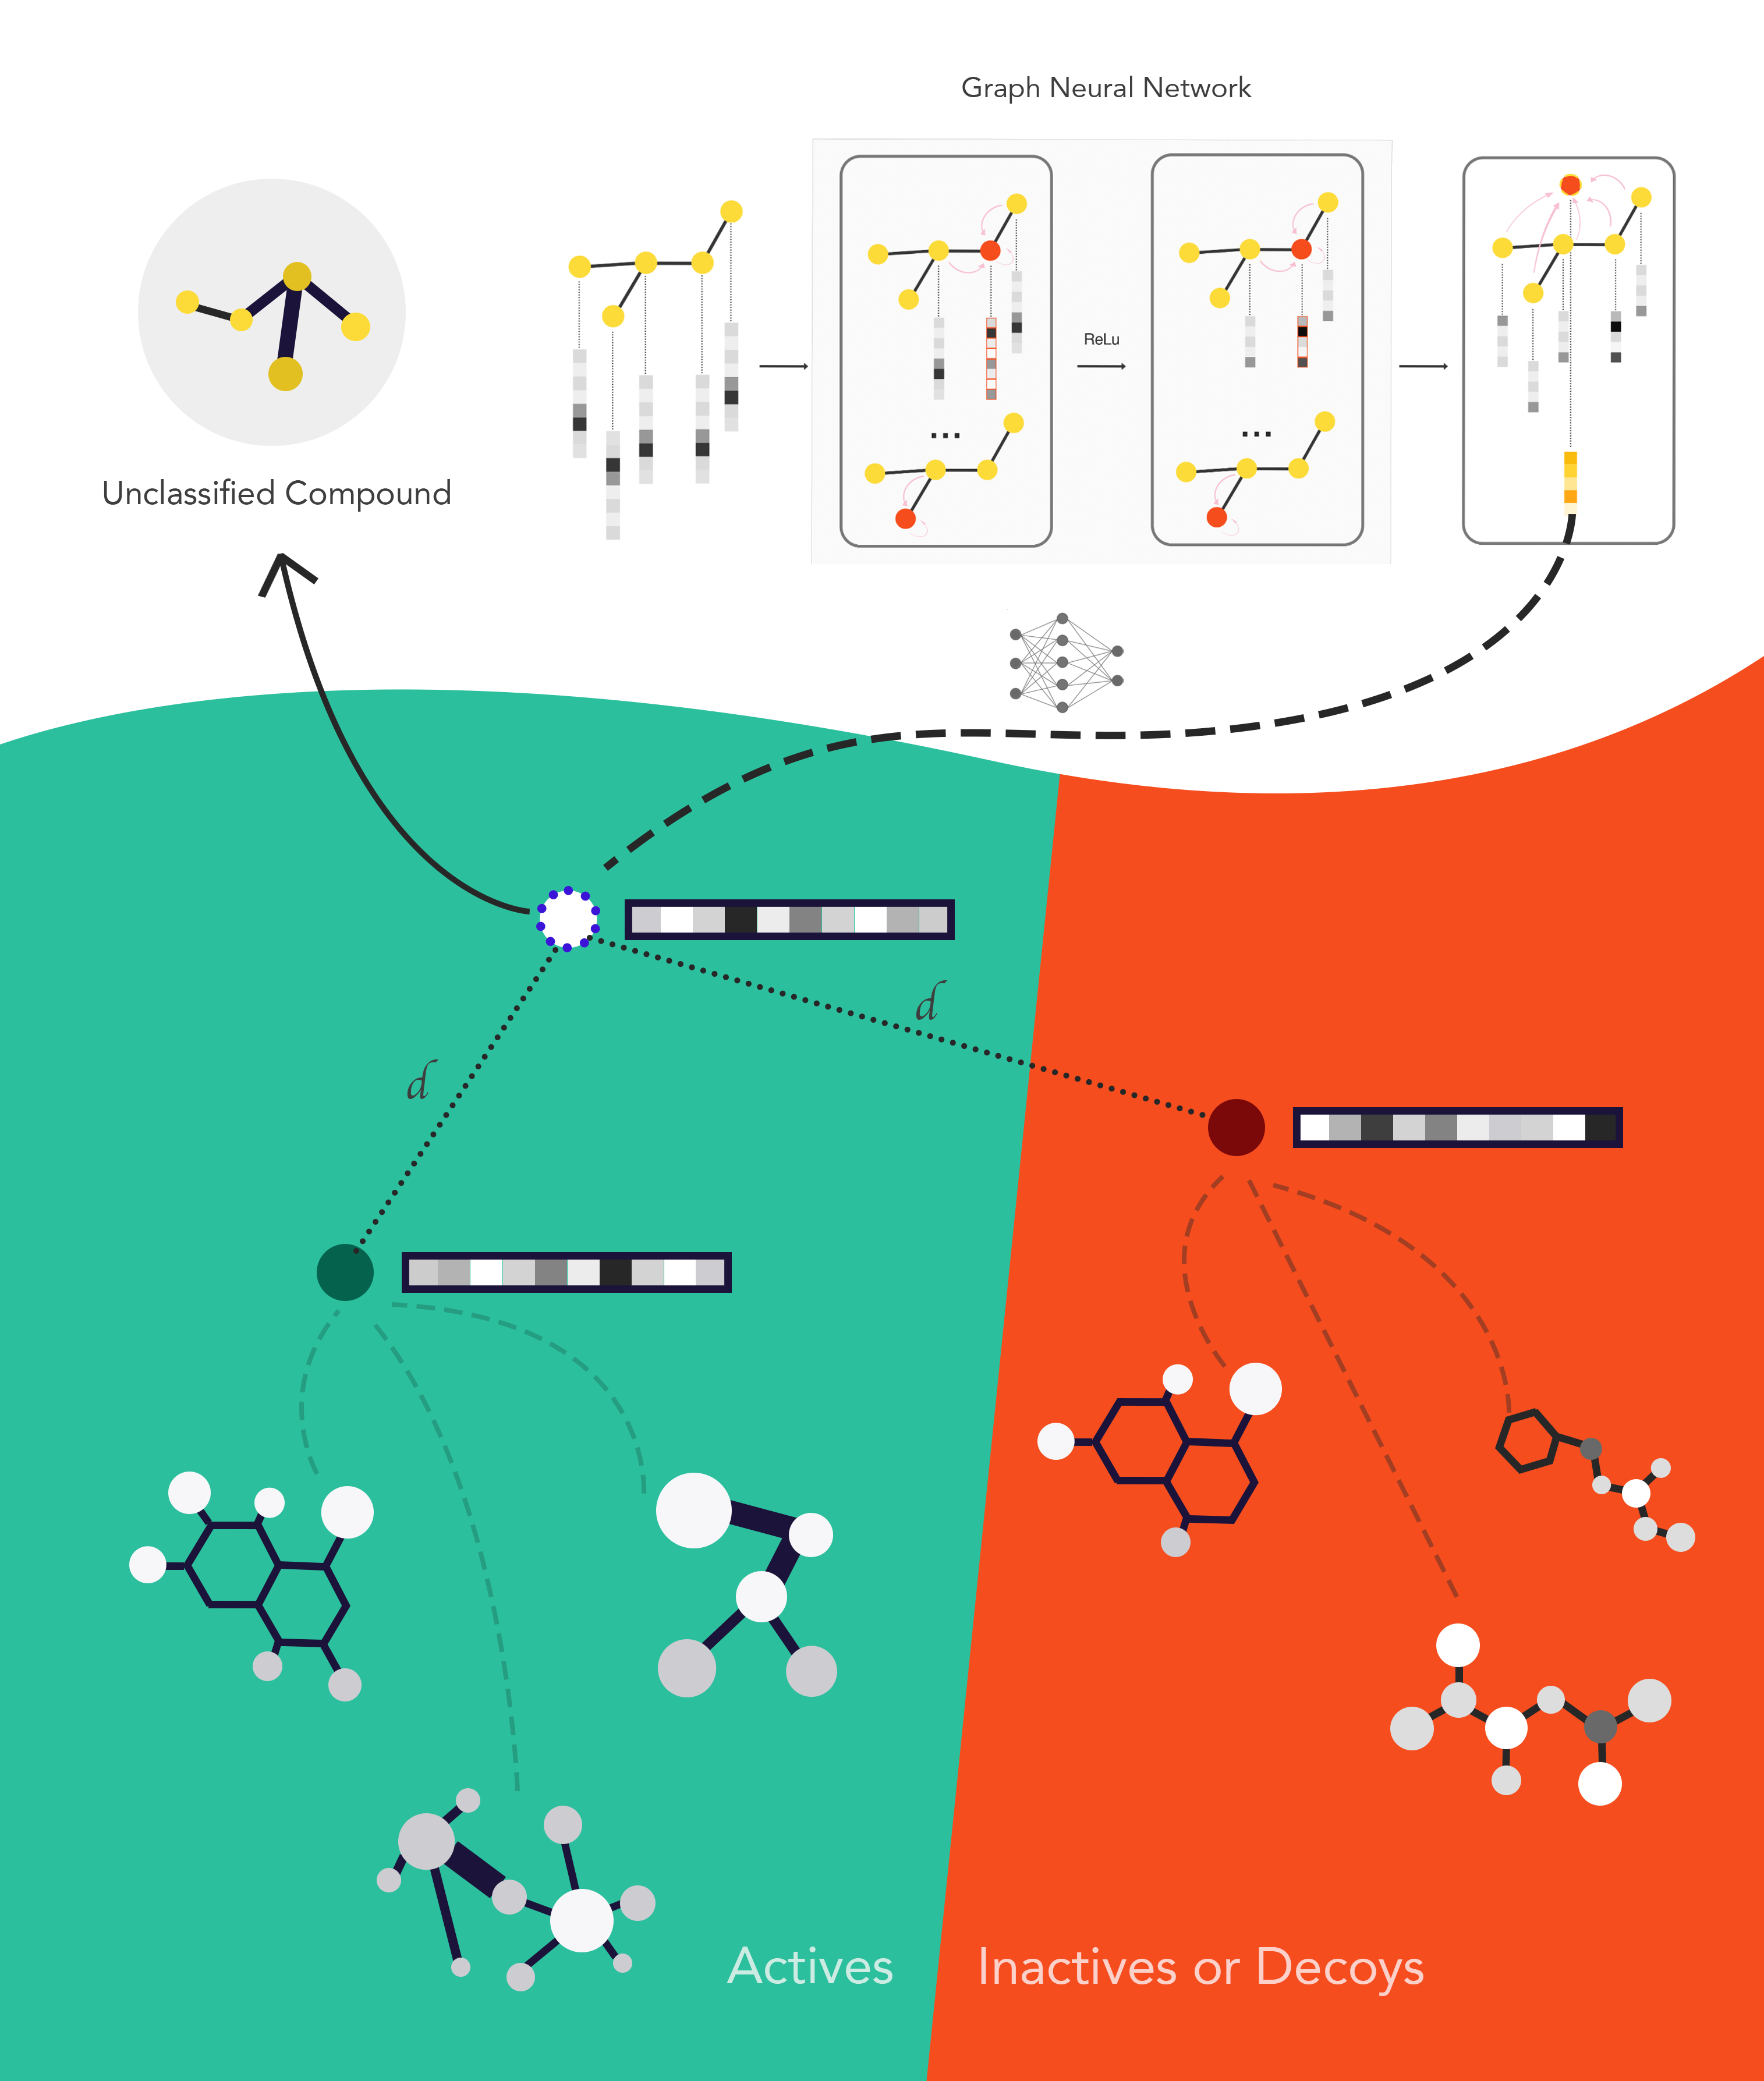
\includegraphics[width=0.85\linewidth]{img/For Table of Contents Only.png}
%DIFDELCMD < 	%%%
%DIFDELCMD < \caption{%
{%DIFAUXCMD
\DIFdelFL{Table of Contents/Abstract Graphic for Article}}
%DIFAUXCMD
%DIFDELCMD < \end{figure}
%DIFDELCMD < 

%DIFDELCMD < %%%
\DIFdelend %%%%%%%%%%%%%%%%%%%%%%%%%%%%%%%%%%%%%%%%%%%%%%%%%%%%%%%%%%%%%%%%%%%%%
%% The appropriate \bibliography command should be placed here.
%% Notice that the class file automatically sets \bibliographystyle
%% and also names the section correctly.
%%%%%%%%%%%%%%%%%%%%%%%%%%%%%%%%%%%%%%%%%%%%%%%%%%%%%%%%%%%%%%%%%%%%%
\providecommand{\latin}[1]{#1}
\makeatletter
\providecommand{\doi}
  {\begingroup\let\do\@makeother\dospecials
  \catcode`\{=1 \catcode`\}=2 \doi@aux}
\providecommand{\doi@aux}[1]{\endgroup\texttt{#1}}
\makeatother
\providecommand*\mcitethebibliography{\thebibliography}
\csname @ifundefined\endcsname{endmcitethebibliography}
  {\let\endmcitethebibliography\endthebibliography}{}
\DIFdelbegin %DIFDELCMD < \begin{mcitethebibliography}{35}
%DIFDELCMD < %%%
\DIFdelend \DIFaddbegin \begin{mcitethebibliography}{34}
\DIFaddend \providecommand*\natexlab[1]{#1}
\providecommand*\mciteSetBstSublistMode[1]{}
\providecommand*\mciteSetBstMaxWidthForm[2]{}
\providecommand*\mciteBstWouldAddEndPuncttrue
  {\def\EndOfBibitem{\unskip.}}
\providecommand*\mciteBstWouldAddEndPunctfalse
  {\let\EndOfBibitem\relax}
\providecommand*\mciteSetBstMidEndSepPunct[3]{}
\providecommand*\mciteSetBstSublistLabelBeginEnd[3]{}
\providecommand*\EndOfBibitem{}
\mciteSetBstSublistMode{f}
\mciteSetBstMaxWidthForm{subitem}{(\alph{mcitesubitemcount})}
\mciteSetBstSublistLabelBeginEnd
  {\mcitemaxwidthsubitemform\space}
  {\relax}
  {\relax}

\bibitem[Hughes \latin{et~al.}(2011)Hughes, Rees, Kalindjian, and
  Philpott]{hughes2011principles}
Hughes,~J.~P.; Rees,~S.; Kalindjian,~S.~B.; Philpott,~K.~L. Principles of early
  drug discovery. \emph{British journal of pharmacology} \textbf{2011},
  \emph{162}, 1239--1249\relax
\mciteBstWouldAddEndPuncttrue
\mciteSetBstMidEndSepPunct{\mcitedefaultmidpunct}
{\mcitedefaultendpunct}{\mcitedefaultseppunct}\relax
\EndOfBibitem
\bibitem[Waring \latin{et~al.}(2015)Waring, Arrowsmith, Leach, Leeson,
  Mandrell, Owen, Pairaudeau, Pennie, Pickett, Wang, \latin{et~al.}
  others]{waring2015analysis}
Waring,~M.~J.; Arrowsmith,~J.; Leach,~A.~R.; Leeson,~P.~D.; Mandrell,~S.;
  Owen,~R.~M.; Pairaudeau,~G.; Pennie,~W.~D.; Pickett,~S.~D.; Wang,~J.,
  \latin{et~al.}  An analysis of the attrition of drug candidates from four
  major pharmaceutical companies. \emph{Nature reviews Drug discovery}
  \textbf{2015}, \emph{14}, 475--486\relax
\mciteBstWouldAddEndPuncttrue
\mciteSetBstMidEndSepPunct{\mcitedefaultmidpunct}
{\mcitedefaultendpunct}{\mcitedefaultseppunct}\relax
\EndOfBibitem
\bibitem[Altae-Tran \latin{et~al.}(2017)Altae-Tran, Ramsundar, Pappu, and
  Pande]{altae2017low}
Altae-Tran,~H.; Ramsundar,~B.; Pappu,~A.~S.; Pande,~V. Low data drug discovery
  with one-shot learning. \emph{ACS central science} \textbf{2017}, \emph{3},
  283--293\relax
\mciteBstWouldAddEndPuncttrue
\mciteSetBstMidEndSepPunct{\mcitedefaultmidpunct}
{\mcitedefaultendpunct}{\mcitedefaultseppunct}\relax
\EndOfBibitem
\bibitem[Koch \latin{et~al.}(2015)Koch, Zemel, Salakhutdinov, \latin{et~al.}
  others]{koch2015siamese}
Koch,~G.; Zemel,~R.; Salakhutdinov,~R., \latin{et~al.}  Siamese neural networks
  for one-shot image recognition. ICML deep learning workshop. 2015\relax
\mciteBstWouldAddEndPuncttrue
\mciteSetBstMidEndSepPunct{\mcitedefaultmidpunct}
{\mcitedefaultendpunct}{\mcitedefaultseppunct}\relax
\EndOfBibitem
\bibitem[Vinyals \latin{et~al.}(2016)Vinyals, Blundell, Lillicrap, Wierstra,
  \latin{et~al.} others]{vinyals2016matching}
Vinyals,~O.; Blundell,~C.; Lillicrap,~T.; Wierstra,~D., \latin{et~al.}
  Matching networks for one shot learning. \emph{Advances in neural information
  processing systems} \textbf{2016}, \emph{29}, 3630--3638\relax
\mciteBstWouldAddEndPuncttrue
\mciteSetBstMidEndSepPunct{\mcitedefaultmidpunct}
{\mcitedefaultendpunct}{\mcitedefaultseppunct}\relax
\EndOfBibitem
\bibitem[Snell \latin{et~al.}(2017)Snell, Swersky, and
  Zemel]{snell2017prototypical}
Snell,~J.; Swersky,~K.; Zemel,~R.~S. Prototypical networks for few-shot
  learning. \emph{arXiv preprint arXiv:1703.05175} \textbf{2017}, \relax
\mciteBstWouldAddEndPunctfalse
\mciteSetBstMidEndSepPunct{\mcitedefaultmidpunct}
{}{\mcitedefaultseppunct}\relax
\EndOfBibitem
\bibitem[Sung \latin{et~al.}(2018)Sung, Yang, Zhang, Xiang, Torr, and
  Hospedales]{sung2018learning}
Sung,~F.; Yang,~Y.; Zhang,~L.; Xiang,~T.; Torr,~P.~H.; Hospedales,~T.~M.
  Learning to compare: Relation network for few-shot learning. Proceedings of
  the IEEE conference on computer vision and pattern recognition. 2018; pp
  1199--1208\relax
\mciteBstWouldAddEndPuncttrue
\mciteSetBstMidEndSepPunct{\mcitedefaultmidpunct}
{\mcitedefaultendpunct}{\mcitedefaultseppunct}\relax
\EndOfBibitem
\bibitem[Wang \latin{et~al.}(2020)Wang, Yao, Kwok, and
  Ni]{wang2020generalizing}
Wang,~Y.; Yao,~Q.; Kwok,~J.~T.; Ni,~L.~M. Generalizing from a few examples: A
  survey on few-shot learning. \emph{ACM Computing Surveys (CSUR)}
  \textbf{2020}, \emph{53}, 1--34\relax
\mciteBstWouldAddEndPuncttrue
\mciteSetBstMidEndSepPunct{\mcitedefaultmidpunct}
{\mcitedefaultendpunct}{\mcitedefaultseppunct}\relax
\EndOfBibitem
\bibitem[Huang \latin{et~al.}(2016)Huang, Xia, Nguyen, Zhao, Sakamuru, Zhao,
  Shahane, Rossoshek, and Simeonov]{huang2016tox21challenge}
Huang,~R.; Xia,~M.; Nguyen,~D.-T.; Zhao,~T.; Sakamuru,~S.; Zhao,~J.;
  Shahane,~S.~A.; Rossoshek,~A.; Simeonov,~A. Tox21Challenge to build
  predictive models of nuclear receptor and stress response pathways as
  mediated by exposure to environmental chemicals and drugs. \emph{Frontiers in
  Environmental Science} \textbf{2016}, \emph{3}, 85\relax
\mciteBstWouldAddEndPuncttrue
\mciteSetBstMidEndSepPunct{\mcitedefaultmidpunct}
{\mcitedefaultendpunct}{\mcitedefaultseppunct}\relax
\EndOfBibitem
\bibitem[Rogers and Hahn(2010)Rogers, and Hahn]{rogers2010extended}
Rogers,~D.; Hahn,~M. Extended-connectivity fingerprints. \emph{Journal of
  chemical information and modeling} \textbf{2010}, \emph{50}, 742--754\relax
\mciteBstWouldAddEndPuncttrue
\mciteSetBstMidEndSepPunct{\mcitedefaultmidpunct}
{\mcitedefaultendpunct}{\mcitedefaultseppunct}\relax
\EndOfBibitem
\bibitem[Duvenaud \latin{et~al.}(2015)Duvenaud, Maclaurin,
  Aguilera-Iparraguirre, G{\'o}mez-Bombarelli, Hirzel, Aspuru-Guzik, and
  Adams]{duvenaud2015convolutional}
Duvenaud,~D.; Maclaurin,~D.; Aguilera-Iparraguirre,~J.;
  G{\'o}mez-Bombarelli,~R.; Hirzel,~T.; Aspuru-Guzik,~A.; Adams,~R.~P.
  Convolutional networks on graphs for learning molecular fingerprints.
  \emph{arXiv preprint arXiv:1509.09292} \textbf{2015}, \relax
\mciteBstWouldAddEndPunctfalse
\mciteSetBstMidEndSepPunct{\mcitedefaultmidpunct}
{}{\mcitedefaultseppunct}\relax
\EndOfBibitem
\bibitem[David \latin{et~al.}(2020)David, Thakkar, Mercado, and
  Engkvist]{david2020molecular}
David,~L.; Thakkar,~A.; Mercado,~R.; Engkvist,~O. Molecular representations in
  AI-driven drug discovery: a review and practical guide. \emph{Journal of
  Cheminformatics} \textbf{2020}, \emph{12}, 1--22\relax
\mciteBstWouldAddEndPuncttrue
\mciteSetBstMidEndSepPunct{\mcitedefaultmidpunct}
{\mcitedefaultendpunct}{\mcitedefaultseppunct}\relax
\EndOfBibitem
\bibitem[Wu \latin{et~al.}(2018)Wu, Ramsundar, Feinberg, Gomes, Geniesse,
  Pappu, Leswing, and Pande]{wu2018moleculenet}
Wu,~Z.; Ramsundar,~B.; Feinberg,~E.~N.; Gomes,~J.; Geniesse,~C.; Pappu,~A.~S.;
  Leswing,~K.; Pande,~V. MoleculeNet: a benchmark for molecular machine
  learning. \emph{Chemical science} \textbf{2018}, \emph{9}, 513--530\relax
\mciteBstWouldAddEndPuncttrue
\mciteSetBstMidEndSepPunct{\mcitedefaultmidpunct}
{\mcitedefaultendpunct}{\mcitedefaultseppunct}\relax
\EndOfBibitem
\bibitem[Jiang \latin{et~al.}(2021)Jiang, Wu, Hsieh, Chen, Liao, Wang, Shen,
  Cao, Wu, and Hou]{jiang2021could}
Jiang,~D.; Wu,~Z.; Hsieh,~C.-Y.; Chen,~G.; Liao,~B.; Wang,~Z.; Shen,~C.;
  Cao,~D.; Wu,~J.; Hou,~T. Could graph neural networks learn better molecular
  representation for drug discovery? A comparison study of descriptor-based and
  graph-based models. \emph{Journal of cheminformatics} \textbf{2021},
  \emph{13}, 1--23\relax
\mciteBstWouldAddEndPuncttrue
\mciteSetBstMidEndSepPunct{\mcitedefaultmidpunct}
{\mcitedefaultendpunct}{\mcitedefaultseppunct}\relax
\EndOfBibitem
\bibitem[G{\'o}mez-Bombarelli \latin{et~al.}(2018)G{\'o}mez-Bombarelli, Wei,
  Duvenaud, Hern{\'a}ndez-Lobato, S{\'a}nchez-Lengeling, Sheberla,
  Aguilera-Iparraguirre, Hirzel, Adams, and Aspuru-Guzik]{gomez2018automatic}
G{\'o}mez-Bombarelli,~R.; Wei,~J.~N.; Duvenaud,~D.;
  Hern{\'a}ndez-Lobato,~J.~M.; S{\'a}nchez-Lengeling,~B.; Sheberla,~D.;
  Aguilera-Iparraguirre,~J.; Hirzel,~T.~D.; Adams,~R.~P.; Aspuru-Guzik,~A.
  Automatic chemical design using a data-driven continuous representation of
  molecules. \emph{ACS central science} \textbf{2018}, \emph{4}, 268--276\relax
\mciteBstWouldAddEndPuncttrue
\mciteSetBstMidEndSepPunct{\mcitedefaultmidpunct}
{\mcitedefaultendpunct}{\mcitedefaultseppunct}\relax
\EndOfBibitem
\bibitem[Bronstein \latin{et~al.}(2021)Bronstein, Bruna, Cohen, and
  Veli{\v{c}}kovi{\'c}]{bronstein2021geometric}
Bronstein,~M.~M.; Bruna,~J.; Cohen,~T.; Veli{\v{c}}kovi{\'c},~P. Geometric deep
  learning: Grids, groups, graphs, geodesics, and gauges. \emph{arXiv preprint
  arXiv:2104.13478} \textbf{2021}, \relax
\mciteBstWouldAddEndPunctfalse
\mciteSetBstMidEndSepPunct{\mcitedefaultmidpunct}
{}{\mcitedefaultseppunct}\relax
\EndOfBibitem
\DIFdelbegin \bibitem[Bromley \latin{et~al.}(1993)Bromley, Bentz, Bottou, Guyon, LeCun,
  Moore, S{\"a}ckinger, and Shah]{bromley1993signature}
\DIFdel{Bromley,~J.; Bentz,~J.~W.; Bottou,~L.; Guyon,~I.; LeCun,~Y.; Moore,~C.;
  S}%DIFDELCMD < {%%%
\DIFdel{\"a}%DIFDELCMD < }%%%
\DIFdel{ckinger,~E.; Shah,~R. Signature verification using a “siamese” time
  delay neural network. }\emph{\DIFdel{International Journal of Pattern Recognition and
  Artificial Intelligence}} %DIFAUXCMD
\textbf{\DIFdel{1993}}%DIFAUXCMD
\DIFdel{, }\emph{\DIFdel{7}}%DIFAUXCMD
\DIFdel{, 669--688}%DIFDELCMD < \relax
%DIFDELCMD < \mciteBstWouldAddEndPuncttrue
%DIFDELCMD < \mciteSetBstMidEndSepPunct{\mcitedefaultmidpunct}
%DIFDELCMD < {\mcitedefaultendpunct}{\mcitedefaultseppunct}\relax
%DIFDELCMD < \EndOfBibitem
%DIFDELCMD < %%%
\DIFdelend \bibitem[LeCun \latin{et~al.}(1995)LeCun, Bengio, \latin{et~al.}
  others]{lecun1995convolutional}
LeCun,~Y.; Bengio,~Y., \latin{et~al.}  Convolutional networks for images,
  speech, and time series. \emph{The handbook of brain theory and neural
  networks} \textbf{1995}, \emph{3361}, 1995\relax
\mciteBstWouldAddEndPuncttrue
\mciteSetBstMidEndSepPunct{\mcitedefaultmidpunct}
{\mcitedefaultendpunct}{\mcitedefaultseppunct}\relax
\EndOfBibitem
\bibitem[Kuhn \latin{et~al.}(2016)Kuhn, Letunic, Jensen, and
  Bork]{kuhn2016sider}
Kuhn,~M.; Letunic,~I.; Jensen,~L.~J.; Bork,~P. The SIDER database of drugs and
  side effects. \emph{Nucleic acids research} \textbf{2016}, \emph{44},
  D1075--D1079\relax
\mciteBstWouldAddEndPuncttrue
\mciteSetBstMidEndSepPunct{\mcitedefaultmidpunct}
{\mcitedefaultendpunct}{\mcitedefaultseppunct}\relax
\EndOfBibitem
\bibitem[Rohrer and Baumann(2009)Rohrer, and Baumann]{rohrer2009maximum}
Rohrer,~S.~G.; Baumann,~K. Maximum unbiased validation (MUV) data sets for
  virtual screening based on PubChem bioactivity data. \emph{Journal of
  chemical information and modeling} \textbf{2009}, \emph{49}, 169--184\relax
\mciteBstWouldAddEndPuncttrue
\mciteSetBstMidEndSepPunct{\mcitedefaultmidpunct}
{\mcitedefaultendpunct}{\mcitedefaultseppunct}\relax
\EndOfBibitem
\bibitem[Kipf and Welling(2016)Kipf, and Welling]{kipf2016semi}
Kipf,~T.~N.; Welling,~M. Semi-Supervised Classification with Graph
  Convolutional Networks. \emph{arXiv preprint arXiv:1609.02907} \textbf{2016},
  \relax
\mciteBstWouldAddEndPunctfalse
\mciteSetBstMidEndSepPunct{\mcitedefaultmidpunct}
{}{\mcitedefaultseppunct}\relax
\EndOfBibitem
\bibitem[Ramsundar \latin{et~al.}(2019)Ramsundar, Eastman, Walters, and
  Pande]{ramsundar2019deep}
Ramsundar,~B.; Eastman,~P.; Walters,~P.; Pande,~V. \emph{Deep learning for the
  life sciences: applying deep learning to genomics, microscopy, drug
  discovery, and more}; " O'Reilly Media, Inc.", 2019\relax
\mciteBstWouldAddEndPuncttrue
\mciteSetBstMidEndSepPunct{\mcitedefaultmidpunct}
{\mcitedefaultendpunct}{\mcitedefaultseppunct}\relax
\EndOfBibitem
\bibitem[NIH(2014)]{tox21}
NIH, Tox21 Data Challenge 2014. 2014; Accessed on 20.08.2021\relax
\mciteBstWouldAddEndPuncttrue
\mciteSetBstMidEndSepPunct{\mcitedefaultmidpunct}
{\mcitedefaultendpunct}{\mcitedefaultseppunct}\relax
\EndOfBibitem
\bibitem[Mysinger \latin{et~al.}(2012)Mysinger, Carchia, Irwin, and
  Shoichet]{mysinger2012directory}
Mysinger,~M.~M.; Carchia,~M.; Irwin,~J.~J.; Shoichet,~B.~K. Directory of useful
  decoys, enhanced (DUD-E): better ligands and decoys for better benchmarking.
  \emph{Journal of medicinal chemistry} \textbf{2012}, \emph{55},
  6582--6594\relax
\mciteBstWouldAddEndPuncttrue
\mciteSetBstMidEndSepPunct{\mcitedefaultmidpunct}
{\mcitedefaultendpunct}{\mcitedefaultseppunct}\relax
\EndOfBibitem
\bibitem[Bento \latin{et~al.}(2020)Bento, Hersey, F{\'e}lix, Landrum, Gaulton,
  Atkinson, Bellis, De~Veij, and Leach]{bento2020open}
Bento,~A.~P.; Hersey,~A.; F{\'e}lix,~E.; Landrum,~G.; Gaulton,~A.;
  Atkinson,~F.; Bellis,~L.~J.; De~Veij,~M.; Leach,~A.~R. An open source
  chemical structure curation pipeline using RDKit. \emph{Journal of
  Cheminformatics} \textbf{2020}, \emph{12}, 1--16\relax
\mciteBstWouldAddEndPuncttrue
\mciteSetBstMidEndSepPunct{\mcitedefaultmidpunct}
{\mcitedefaultendpunct}{\mcitedefaultseppunct}\relax
\EndOfBibitem
\bibitem[RDKit(2012)]{rdkit}
RDKit, Open-source cheminformatics. https://www.rdkit.org. 2012; Last Accessed
  on 25/11/2021\relax
\mciteBstWouldAddEndPuncttrue
\mciteSetBstMidEndSepPunct{\mcitedefaultmidpunct}
{\mcitedefaultendpunct}{\mcitedefaultseppunct}\relax
\EndOfBibitem
\bibitem[Brecher(2006)]{brecher2006graphical}
Brecher,~J. Graphical representation of stereochemical configuration (IUPAC
  Recommendations 2006). \emph{Pure and applied chemistry} \textbf{2006},
  \emph{78}, 1897--1970\relax
\mciteBstWouldAddEndPuncttrue
\mciteSetBstMidEndSepPunct{\mcitedefaultmidpunct}
{\mcitedefaultendpunct}{\mcitedefaultseppunct}\relax
\EndOfBibitem
\bibitem[Food and Administration(2007)Food, and
  Administration]{food2007substance}
Food,~F.; Administration,~D. Substance Definition Manual. \emph{Standard
  Operating Procedure, “Substance Definition Manual,” Version 5c}
  \textbf{2007}, \emph{94}\relax
\mciteBstWouldAddEndPuncttrue
\mciteSetBstMidEndSepPunct{\mcitedefaultmidpunct}
{\mcitedefaultendpunct}{\mcitedefaultseppunct}\relax
\EndOfBibitem
\bibitem[Mufei \latin{et~al.}(2021)Mufei, Jinjing, Jiajing, Wenxuan, Yangkang,
  Yaxin, and George]{dgllife}
Mufei,~L.; Jinjing,~Z.; Jiajing,~H.; Wenxuan,~F.; Yangkang,~Z.; Yaxin,~G.;
  George,~K. DGL-LifeSci: An Open-Source Toolkit for Deep Learning on Graphs in
  Life Science. \emph{arXiv preprint arXiv:2106.14232} \textbf{2021}, \relax
\mciteBstWouldAddEndPunctfalse
\mciteSetBstMidEndSepPunct{\mcitedefaultmidpunct}
{}{\mcitedefaultseppunct}\relax
\EndOfBibitem
\bibitem[Wang \latin{et~al.}(2019)Wang, Zheng, Ye, Gan, Li, Song, Zhou, Ma, Yu,
  Gai, Xiao, He, Karypis, Li, and Zhang]{wang2019dgl}
Wang,~M.; Zheng,~D.; Ye,~Z.; Gan,~Q.; Li,~M.; Song,~X.; Zhou,~J.; Ma,~C.;
  Yu,~L.; Gai,~Y.; Xiao,~T.; He,~T.; Karypis,~G.; Li,~J.; Zhang,~Z. Deep Graph
  Library: A Graph-Centric, Highly-Performant Package for Graph Neural
  Networks. \emph{arXiv preprint arXiv:1909.01315} \textbf{2019}, \relax
\mciteBstWouldAddEndPunctfalse
\mciteSetBstMidEndSepPunct{\mcitedefaultmidpunct}
{}{\mcitedefaultseppunct}\relax
\EndOfBibitem
\bibitem[Mann and Whitney(1947)Mann, and Whitney]{mann1947test}
Mann,~H.~B.; Whitney,~D.~R. On a test of whether one of two random variables is
  stochastically larger than the other. \emph{The annals of mathematical
  statistics} \textbf{1947}, 50--60\relax
\mciteBstWouldAddEndPuncttrue
\mciteSetBstMidEndSepPunct{\mcitedefaultmidpunct}
{\mcitedefaultendpunct}{\mcitedefaultseppunct}\relax
\EndOfBibitem
\bibitem[Smusz \latin{et~al.}(2013)Smusz, Kurczab, and
  Bojarski]{smusz2013influence}
Smusz,~S.; Kurczab,~R.; Bojarski,~A.~J. The influence of the inactives subset
  generation on the performance of machine learning methods. \emph{Journal of
  cheminformatics} \textbf{2013}, \emph{5}, 1--8\relax
\mciteBstWouldAddEndPuncttrue
\mciteSetBstMidEndSepPunct{\mcitedefaultmidpunct}
{\mcitedefaultendpunct}{\mcitedefaultseppunct}\relax
\EndOfBibitem
\bibitem[Wallach and Heifets(2018)Wallach, and Heifets]{wallach2018most}
Wallach,~I.; Heifets,~A. Most ligand-based classification benchmarks reward
  memorization rather than generalization. \emph{Journal of chemical
  information and modeling} \textbf{2018}, \emph{58}, 916--932\relax
\mciteBstWouldAddEndPuncttrue
\mciteSetBstMidEndSepPunct{\mcitedefaultmidpunct}
{\mcitedefaultendpunct}{\mcitedefaultseppunct}\relax
\EndOfBibitem
\bibitem[Chen \latin{et~al.}(2019)Chen, Cruz, Ramsey, Dickson, Duca, Hornak,
  Koes, and Kurtzman]{chen2019hidden}
Chen,~L.; Cruz,~A.; Ramsey,~S.; Dickson,~C.~J.; Duca,~J.~S.; Hornak,~V.;
  Koes,~D.~R.; Kurtzman,~T. Hidden bias in the DUD-E dataset leads to
  misleading performance of deep learning in structure-based virtual screening.
  \emph{PloS one} \textbf{2019}, \emph{14}, e0220113\relax
\mciteBstWouldAddEndPuncttrue
\mciteSetBstMidEndSepPunct{\mcitedefaultmidpunct}
{\mcitedefaultendpunct}{\mcitedefaultseppunct}\relax
\EndOfBibitem
\end{mcitethebibliography}
\DIFaddbegin 


\pagebreak
\section{\DIFadd{For Table of Contents Only}}

\begin{figure}[!ht]
	\centering
	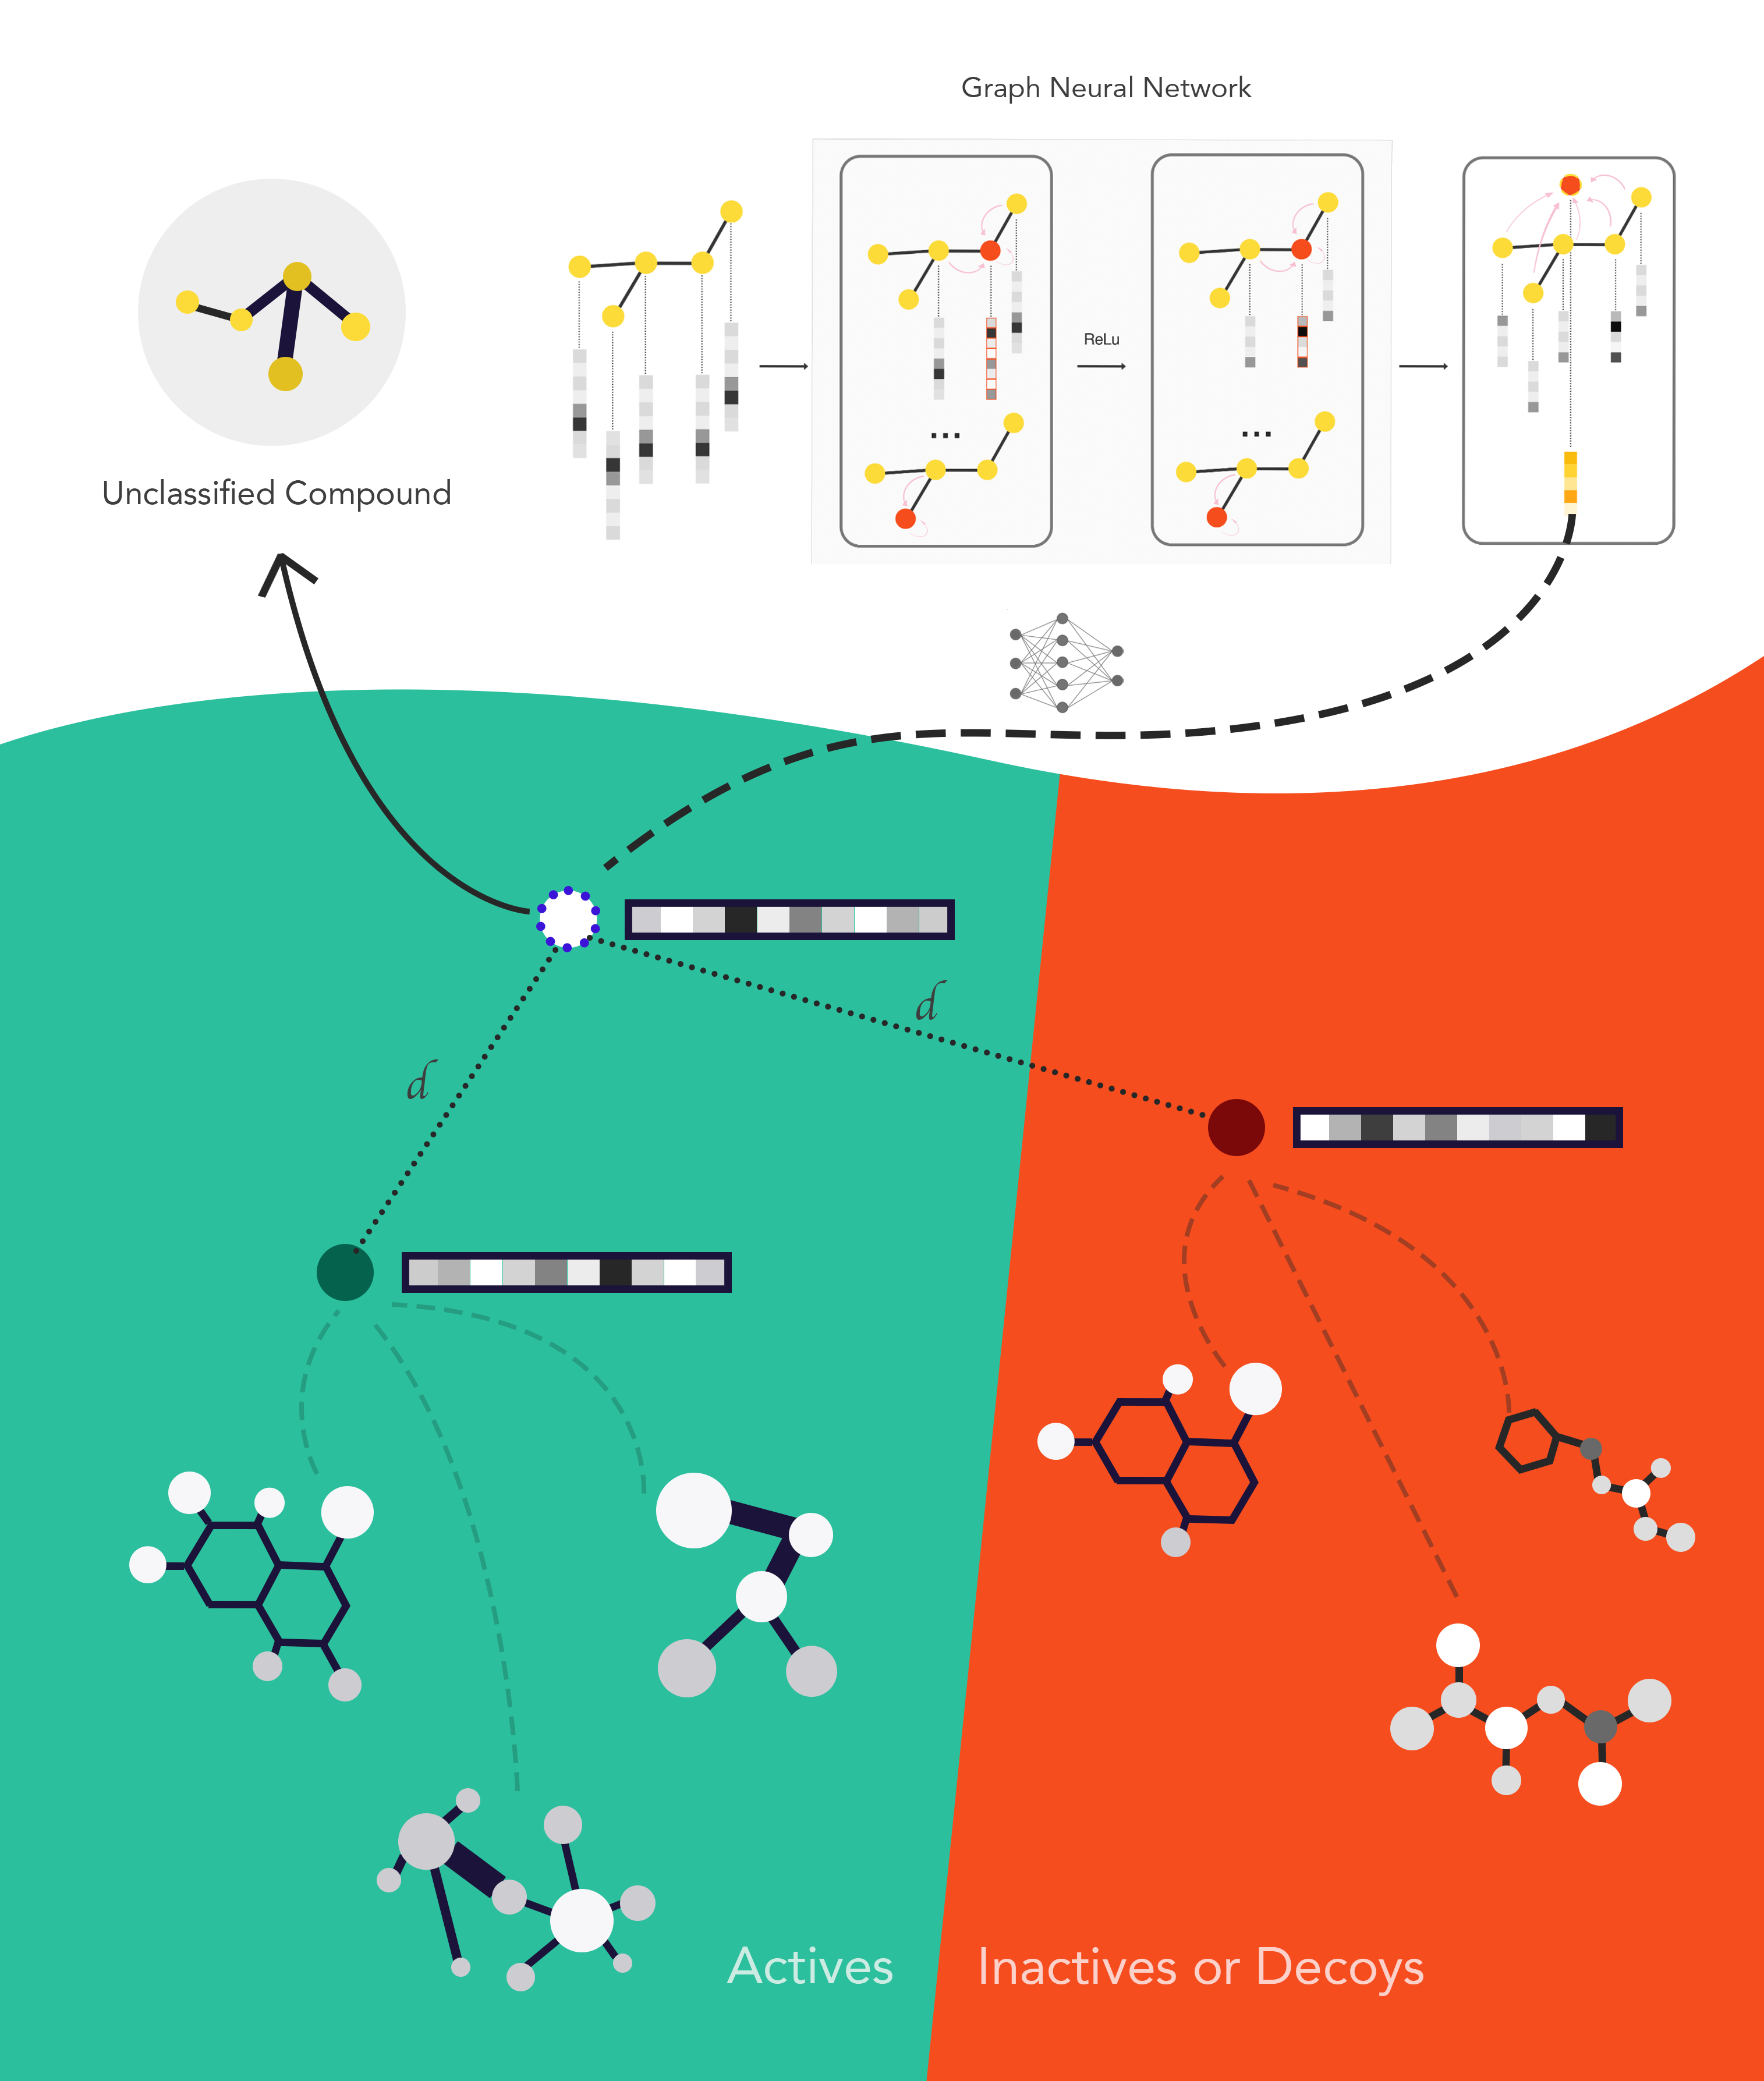
\includegraphics[width=0.95\linewidth]{img/For Table of Contents Only.png}
%DIF > %	\caption{Table of Contents/Abstract Graphic for Article}
\end{figure}
\DIFaddend 


\end{document}
